\include{header}


\begin{document}
\bibliographystyle{ieeetran}
\title{Projektarbeit 2019}
\author{Dano Roost & Ralph Meier}

%\setmainfont{TeX Gyre Pagella}
\begin{titlepage}

% Logo
\ThisTileWallPaper{\paperwidth}{\paperheight}{images/logos/InIT.pdf} % {images/logos/*.pdf}
% Wählen Sie aus folenden pdf Files: ICP, IDP, IEFE, IMES, IMPE, IMS, INE, InES, InIT, KSR, SoE, ZAMP, ZAV, ZIL, ZPP, ZSN

\begin{minipage}[b]{0.117\textwidth}
\hskip 0.05cm
\end{minipage}
\begin{minipage}[b]{0.91\textwidth}
\begin{tiny}.\end{tiny}\vskip 2.8cm
	{\huge
	
	% Projekt Name
	\textbf{\underline{Project thesis (Computer Science)}}\\

	% Projekt Titel
	Reinforcement Learning mit einem Multi-Agenten System für die Planung von Zügen
	\vskip 0.5cm}
	
	\begin{minipage}[b]{0.27\textwidth}
	\hrule\vskip 0.5cm
		\textbf{Authors}\\
		\\
	\end{minipage}
	\begin{minipage}[b]{0.03\textwidth}
	\hskip 0.5cm
	\end{minipage}
	\begin{minipage}[b]{0.7\textwidth}
	\hrule\vskip 0.5cm
		Dano Roost\\
		Ralph Meier\\
	\end{minipage}
	
	\begin{minipage}[b]{0.27\textwidth}
	\hrule\vskip 0.5cm
		\textbf{Main supervisor}\\
		\\
	\end{minipage}
	\begin{minipage}[b]{0.03\textwidth}
	\hskip 0.5cm
	\end{minipage}
	\begin{minipage}[b]{0.7\textwidth}
	\hrule\vskip 0.5cm
		Andreas Weiler\\
        \\
	\end{minipage}
	
	\begin{minipage}[b]{0.27\textwidth}
	\hrule\vskip 0.5cm
		\textbf{Sub supervisor}\\
		\\
	\end{minipage}
	\begin{minipage}[b]{0.03\textwidth}
	\hskip 0.5cm
	\end{minipage}
	\begin{minipage}[b]{0.7\textwidth}
	\hrule\vskip 0.5cm
		Thilo Stadelmann\\
    \\
	\end{minipage}
	
	\begin{minipage}[b]{0.27\textwidth}
	\hrule\vskip 0.5cm
		\textbf{Date}
	\end{minipage}
	\begin{minipage}[b]{0.03\textwidth}
	\hskip 0.5cm
	\end{minipage}
	\begin{minipage}[b]{0.7\textwidth}
	\hrule\vskip 0.5cm
		20.12.2019
	\end{minipage}
\end{minipage}
\vskip 0.5cm
\end{titlepage}

\setcounter{page}{1}
%\include{content/Kontakt}
%%%%%%%%%%%%%%%%%%%%%%%%%%%%%%%%%%%%%%%%%%%%%%%%%%%%%%%%%%%%%%%%%
%  _____   ____  _____                                          %
% |_   _| /  __||  __ \    Institute of Computitional Physics   %
%   | |  |  /   | |__) |   Zuercher Hochschule Winterthur       %
%   | |  | (    |  ___/    (University of Applied Sciences)     %
%  _| |_ |  \__ | |        8401 Winterthur, Switzerland         %
% |_____| \____||_|                                             %
%%%%%%%%%%%%%%%%%%%%%%%%%%%%%%%%%%%%%%%%%%%%%%%%%%%%%%%%%%%%%%%%%
%
% Project     : LaTeX doc Vorlage für Windows ProTeXt mit TexMakerX
% Title       : 
% File        : abstract.tex Rev. 00
% Date        : 23.4.12
% Author      : Remo Ritzmann
% Feedback bitte an Email: remo.ritzmann@pfunzle.ch
%
%%%%%%%%%%%%%%%%%%%%%%%%%%%%%%%%%%%%%%%%%%%%%%%%%%%%%%%%%%%%%%%%%

\thispagestyle{empty}

\chapter*{Zusammenfassung}\label{chap.zusammenfassung}
\begin{otherlanguage}{nswissgerman}
%1. Einleitung («Problemstellung»): Definiert die Problematik und begründet die Relevanz der Arbeit. Die Situation (eine problematische Situation oder technische Problematik) und die wissenschaftliche/fachliche Untersuchungs-Fragestellung (folgt logischer- weise aus der festgestellten Problematik) werden kurz beschrieben.
Die steigende Anzahl der Pendler bring die Kapazität des Schienennetzes der Schweizerischen Bundesbahnen SBB immer mehr an seine Grenzen. Da der Ausbau der Infrastruktur nicht mit den Passagierzahlen mithalten kann, bemüht sich die SBB, mehr Züge in dichteren Abständen auf ihr Netz zu bringen.
Für die Planung des dichteren Zugverkehrs experimentiert die SBB auch mit Technologien des maschinellen Lernens, insbesondere mit Reinforcement Learning (RL). Dabei soll ein Algorithmus selbstständig Strategien erlernen, um das gegebene Problem zu lösen. In diesem Fall handelt es sich dabei um das Steuern von Zügen, welche möglichst zeitnah zu ihrem Ziel geführt werden sollen. Kollisionen gilt es dabei zu verhindern und potenzielle Hindernisse wie defekte Züge müssen umfahren werden. Auch können Züge mit verschiedenen Geschwindigkeiten unterwegs sein, was bei der Planung berücksichtigt werden soll.\\
Diese Arbeit ist dabei ein Beitrag zur sogenannten Flatland Challenge, einem Wettbewerb der SBB und der Crowdsourcing-Plattform AICrowd, bei welchem das beschriebene Problem mittels einer zur Verfügung gestellten Simulation des Schienennetzes gelöst werden soll. Der Wettbewerb ist aufgeteilt in zwei Runden mit wachsendem Schwierigkeitslevel.
Diese Schienensimulation erlaubt es, eigene Lösungen für das Problem zu trainieren und zu evaluieren. Die Schwierigkeit dabei ist, die Züge so zu steuern, dass sie sich auch in komplexen Situationen nicht blockieren. Dazu ist primär die Zusammenarbeit der Züge von grosser Bedeutung.\\
%3. Vorgehen («Problembehandlung»): Informiert über das Vorgehen und über die Untersuchungsanlage.
Der präsentierte Lösungsansatz verwendet den Asynchronous Advantage Actor Critic Algorithmus (A3C), einen der derzeit besten RL-Algorithmen, welcher verteiltes Lernen ermöglicht. Der präsentierte Ansatz orientiert sich dabei stark an der Ausgangslösung von Stephan Huschauer.
Nach der ersten lauffähigen Version wurde der Ansatz nach und nach mit unterschiedlichen Features erweitert, wie beispielsweise einem veränderten Kontrollmechanismus der Züge, Curriculum Learning oder verteiltem Lernen über mehrere Rechner.
Um den Fortschritt zu quantifizieren wurden für sämtliche Änderungen Experimente durchgeführt. Durch das Hinzufügen unterschiedlicher Features konnte eine signifikante Verbesserung der Performanz verzeichnet werden. In Runde 1 war es dabei möglich, die Ankunftsrate von den 16.6\% der Ausgangslösung auf 48.9\% zu verbessern.
Für die anspruchsvolleren Eisenbahnnetze der 2. Runde, für welche keine Ausgangslösung existiert, konnte dank weiteren Verbesserungen ebenfalls ein respektables Resultat erzielt werden. Die präsentierte Lösung konnte eine Ankunftsrate von 29.1\% erreichen, was zum Evaluierungszeitpunkt dem 4. Platz von insgesamt 24 teilnehmenden Teams entsprach. Für einen praktischen Einsatz ist die präsentierte Lösung jedoch noch nicht geeignet, dies bedarf weiterer Forschung.
\end{otherlanguage}

\NewPage
\thispagestyle{empty}
\chapter*{Abstract}\label{abstract}
The increasing number of commuters is pushing the capacity of the Swiss Federal Railways SBB rail network to its limits. Since the expansion of the infrastructure cannot keep up with the increasing number of passengers, SBB is exploring new ways to bring more trains onto its network. To achieve this goal, SBB is also experimenting with machine learning technologies such as reinforcement learning (RL).
The goal for this type of algorithm is to independently learn strategies  in order to solve the problem at hand, in our case the challenge of guiding trains to their assigned destinations. Besides not colliding with other trains, it is also necessary to avoid potential obstacles such as defective trains and to take different speed profiles into account.\\
This work is a contribution to the Flatland Challenge, a competition published by SBB and the crowdsourcing platform AICrowd, which aims to solve the problem described by using a provided simulation of the rail network. The competition is divided into two rounds with increasing difficulty. This rail simulation allows us to train and evaluate own solutions for the given problem. The main task is to control the trains in cooperative way so they do not block each other even in complex situations. The selected solution uses the Asynchronous Advantage Actor Critic Algorithm (A3C), a state of the art RL algorithm which supports distributed learning. The approach presented is based on the baseline solution presented by Stephan Huschauer. After establishing the first running version, the approach was improved with an array of new features such as a modified train control mechanism, curriculum learning or distributed learning over multiple computers. To quantify the progress, experiments were conducted for all applied changes. By adding these features, a significant improvement could be achieved. In round one, it was possible to improve the train arrival rate from 16.6\% of the baseline solution to 48.9\%.
For the more demanding second round, there is no baseline available. The solution presented was able to achieve a train arrival rate of 29.1\%, which corresponded at submission time to the 4th place of a total of 24 participating teams.
However, the solution presented is not yet suitable for practical use and requires further research to achieve a useful performance in a real-world scenario.

\chapter*{Preface}\label{preface}
We would like to give special thanks to:
\begin{itemize}
    \item Andreas Weiler and Thilo Stadelmann for their great support during this work, for their helpful tips and for pushing us into the right direction.\\
    We are grateful for the opportunity to dive deep into the field of reinforcement learning as part of this project.
    \item Remo Maurer for being very generous with providing computing infrastructure, especially the infrastructure test server.
\end{itemize}




\includepdf{images/Erklaerung_PA.pdf} % Entsprechendes auskommentieren
% \includepdf{images/Erklaerung_PA.pdf}
% \newpage

%Inhaltsverzeichnis
\tableofcontents
\newpage



%\textbf{}
%\setcounter{page}{1}
%\pagenumbering{arabic}

%\input{content/howtoLaTeX} % Für das Schlussdokument auskommentieren

%%%%%%%%%%%%%%%%%%%%%%%%%%%%%%%%%%%%%%%%%%%%%%%%%%%%%%%%%%%%%%%%%
%  _____   ____  _____                                          %
% |_   _| /  __||  __ \    Institute of Computitional Physics   %
%   | |  |  /   | |__) |   Zuercher Hochschule Winterthur       %
%   | |  | (    |  ___/    (University of Applied Sciences)     %
%  _| |_ |  \__ | |        8401 Winterthur, Switzerland         %
% |_____| \____||_|                                             %
%%%%%%%%%%%%%%%%%%%%%%%%%%%%%%%%%%%%%%%%%%%%%%%%%%%%%%%%%%%%%%%%%
%
% Project     : LaTeX doc Vorlage für Windows ProTeXt mit TexMakerX
% Title       : 
% File        : einleitung.tex Rev. 00
% Date        : 23.4.12
% Author      : Remo Ritzmann
% Feedback bitte an Email: remo.ritzmann@pfunzle.ch
%
%%%%%%%%%%%%%%%%%%%%%%%%%%%%%%%%%%%%%%%%%%%%%%%%%%%%%%%%%%%%%%%%%

\chapter{Einleitung}\label{chap.einleitung}


\section{Ausgangslage}\label{ausgangslage}

\begin{itemize}
\item Nennt bestehende Arbeiten/Literatur zum Thema -> Literaturrecherche
\item Stand der Technik: Bisherige Lösungen des Problems und deren Grenzen
\item (Nennt kurz den Industriepartner und/oder weitere Kooperationspartner und dessen/deren Interesse am Thema Fragestellung)
%The target of this work was to let trains find the optimal and fastest path to their target station. \\
The indirect industry partner during this work was the Swiss Federal Railways (SBB AG) which created the challange on AICrowd \cite{Test}.\\ 
The challenge consists of 2 parts. Part 1 was about avoiding conflicts with multiple trains on their given environment. \\
The aim of part 2 was to optimize train traffic which includes train with different speeds, broken trains and less switchover facilities.\\
%TODO: think about writing something about current state at SBB? -> Stand der Technik
\end{itemize}



\section{Zielsetzung / Aufgabenstellung / Anforderungen}\label{zielsetzung}

\begin{itemize}
\item Formuliert das Ziel der Arbeit
\item Verweist auf die offizielle Aufgabenstellung des/der Dozierenden im Anhang
\item (Pflichtenheft, Spezifikation)
\item (Spezifiziert die Anforderungen an das Resultat der Arbeit)
\item (Übersicht über die Arbeit: stellt die folgenden Teile der Arbeit kurz vor)
\item (Angaben zum Zielpublikum: nennt das für die Arbeit vorausgesetzte Wissen)
\item (Terminologie: Definiert die in der Arbeit verwendeten Begriffe)
\end{itemize}


%%%%%%%%%%%%%%%%%%%%%%%%%%%%%%%%%%%%%%%%%%%%%%%%%%%%%%%%%%%%%%%%%
%  _____   ____  _____                                          %
% |_   _| /  __||  __ \    Institute of Computitional Physics   %
%   | |  |  /   | |__) |   Zuercher Hochschule Winterthur       %
%   | |  | (    |  ___/    (University of Applied Sciences)     %
%  _| |_ |  \__ | |        8401 Winterthur, Switzerland         %
% |_____| \____||_|                                             %
%%%%%%%%%%%%%%%%%%%%%%%%%%%%%%%%%%%%%%%%%%%%%%%%%%%%%%%%%%%%%%%%%
%
% Project     : LaTeX doc Vorlage für Windows ProTeXt mit TexMakerX
% Title       : 
% File        : grundlagen.tex Rev. 00
% Date        : 7.5.12
% Author      : Remo Ritzmann
% Feedback bitte an Email: remo.ritzmann@pfunzle.ch
%
%%%%%%%%%%%%%%%%%%%%%%%%%%%%%%%%%%%%%%%%%%%%%%%%%%%%%%%%%%%%%%%%%

\chapter{Technical and mathematical foundation}\label{chap.grundlagen}
\section{Reinforcement learning}\label{projektmanagement}
\subsection*{Basic definitions}\label{basic_rl_definitions}
\begin{itemize}
In recent years, major progress in reinforcement learning has been achieved.
In reinforcement learning, an agent $\mathcal{A}$ learns to perform a task by interacting with an environment $\mathcal{E}$. On every discrete timestep $\mathcal{t}$ the agent needs to take an action $\mathcal{u}$. This action $\mathcal{u}$ is based on the current observation $\mathcal{s}$.
If the agent does well, it receives positive reward from the environment, if it does something bad, there is no or negative reward. The goal of the agent $\mathcal{A}$ is now to maximize the expected future reward  $\EX[\mathcal{R}_{t+1}+\mathcal{R}_{t+1}+\mathcal{R}_{t+1}+...|\mathcal{s}_{t}]$ given the current observation $\mathcal{s}$.\\
The current observation $\mathcal{s}_{t}$, also known as the current state is used to determine which action $\mathcal{u}$ to take next. An agent can observe its environment either fully or partially.\\
\end{itemize}
\subsection*{Value based versus policy based methods}\label{value_policy_based_methods}
\begin{itemize}
Reinforcement learning methods are categorized into value-based methods and policy-based methods. Those variants differ on how they select an action $\mathcal{u}$ from a state $\mathcal{s}$.
Value-based reinforcement learning has its origins in dynamic programming. Through repeated rollouts of the environment, a value function $\mathcal{V(s)}$
is aquired. $\mathcal{V(s)}$ aims to estimate the future expected reward for any given state $\mathcal{s}$ as precisely as possible. This estimation $\mathcal{V(s)}$ is achieved by either a lookup table for all possible states or a function approximator. In this work, we solely focus on the case that $\mathcal{V(s)}$ is implemented in form of a neural network as function approximator. Using this approximation $\mathcal{V(s)}$ we can now select the action $\mathcal{u}$ that takes the agent into the next state $\mathcal{s}_{t+1}$ with the highest expected reward \\
The second category of reinfocement learning algrithms are the so called policy based methods. These methods aim to aquire a stochastic policy $\pi$ that maximizes the expected reward $\mathcal{R}$ by taking actions with certain probabilities. Taking actions based on probabilities solves an important issue of value based methods, which is, that by taking greedy actions with respect to state  $\mathcal{s}$, the agent might not explore the whole state space and misses out on better ways to solve the environment (source!!).
\end{itemize}





Mnih et al, DQN Atari
https://www.cs.toronto.edu/~vmnih/docs/dqn.pdf

Wu et al, A3C
https://arxiv.org/abs/1602.01783

Overview over MARL, Hernandez-Leal et al
https://arxiv.org/pdf/1810.05587.pdf

A3C in a multi agent environment, 
https://arxiv.org/pdf/1903.01365.pdf

 % (2. Theoretische Grundlagen)
\usepackage{hyperref}


%%%%%%%%%%%%%%%%%%%%%%%%%%%%%%%%%%%%%%%%%%%%%%%%%%%%%%%%%%%%%%%%%
%  _____   ____  _____                                          %
% |_   _| /  __||  __ \    Institute of Computitional Physics   %
%   | |  |  /   | |__) |   Zuercher Hochschule Winterthur       %
%   | |  | (    |  ___/    (University of Applied Sciences)     %
%  _| |_ |  \__ | |        8401 Winterthur, Switzerland         %
% |_____| \____||_|                                             %
%%%%%%%%%%%%%%%%%%%%%%%%%%%%%%%%%%%%%%%%%%%%%%%%%%%%%%%%%%%%%%%%%
%
% Project     : LaTeX doc Vorlage für Windows ProTeXt mit TexMakerX
% Title       : 
% File        : vorgehen.tex Rev. 00
% Date        : 7.5.12
%       : Remo Ritzmann
% Feedback bitte an Email: remo.ritzmann@pfunzle.ch
%
%%%%%%%%%%%%%%%%%%%%%%%%%%%%%%%%%%%%%%%%%%%%%%%%%%%%%%%%%%%%%%%%%

\chapter{Basic Implementation}\label{chap.basic_implementation}
\section{A3C Implementation}\label{a3c_implementation}
Originally, the asynchronous advantage actor critic algorithm (A3C) has been designed for use in a single agent environment \cite{a3c}.
By applying it in a multi agent environment, we implicitly convert the environment into a non-stationary system.
While applying A3C in a multi agent setting, the other agents can be viewed as part of the environment. This means, the behaviour of the environment changes while training, due to the fact that the behaviour of the other agents changes.
Gupta et al.finds in \cite{multiagent_comp_a3c_dqn_etc}, that RL methods like Deep Q-networks (DQN) and Trust region policy optimization (TRPO) are not performing well in a multi agent environment, due to the combination of experience replay and non-stationarity of the environment. We therefore suggest, that it is not recommendable to keep an experience replay buffer with older episodes. Otherwise the sampled experience might represent old agent behaviour which is then learned to deal with.\\
An important implementation detail in our version is, that we do not perform updates during episodes but only at their end. The reason for this is, that the only possibility for an agent to receive reward is at the end of the episode. Therefore would any earlier update have a reward of 0 and not help the training process.

\section{Entropy Balancing}\label{entropy_balancing_hyperparameter}
In RL, it is of great importance to find the right combination of exploration and explotation \cite{explorationexploitation}. During exploration, the agent explores as much of the state space as possible. This enables the agent to later exploit the found states which are beneficial. Without this exploration phase, there is a chance that the agent settles on suboptimal policies too quickly and ignores parts of the state space the agent has never seen and therefore does not consider in his action selection. To avoid an early convergence in A3C, it is common to use an additional entropy term. This entropy term is defined as \cite{a3c}:
\begin{gather*}
H(p) = -\sum_{u=0}^{U}log(p_{u})*p_{u}
\end{gather*}
Where $\mathcal{p}$ is a possibility distribution over all available actions $\mathcal{U}$. The entropy is multiplied with a factor $\beta$ and added to the policy loss. This has an effect of preventing a convergence towards a single action, especially in the early phase of training. Without this entropy term, we often observe such an early convergence with grave consequences for the training perfromance. We also observe, that it is recommendable to reduce this factor $\beta$ to zero, once a stage of training is achieved, where it is not nescessary to explore anymore.
\section{Observation Design}\label{enhanced_observations}
The Flatland environment provides a base to build custom observation builders that can be used to create a state representation for the agents as explained in \autoref{observations}. In this work, we do not consider the usage of the grid-based observation builders.
Both the Flatland development team as well as S. Huschauer find, that tree based observations work better in their experiments \cite{flatlandstephan}. The Flatland specification states \cite{flatland_spec}:
\begin{quote}
	Considering, that the actions and directions an agent can chose in any given cell, it becomes clear that a grid like observation around an agent will not contain much useful information, as most of the observed cells are not reachable nor play a significant role in for the agents decisions.
\end{quote}
Based on the provided TreeObsForRailEnv (see \autoref{observations}), we implement a custom observation builder which we use to produce an input vector for our neural network. This observation builder takes the the current state of the environment and produces a fixed size numeric vector with values between 0.0 and 1.0 for each agent. This input vector should fulfil an number of requirements:
\begin{itemize}
	\item Each rail section the agent possibly rides on next should be visible to the agent.
	\item The agent should be able to detect, whether there is another train coming the opposite direction on any section.
	\item The agent should be able to detect on each switch which turn is the faster way to his target.
	\item On switches, the agent should be able to see if a turn does lead to his target, even if it is not the fastest way. If this is the case, taking this turn might even be a good option to evade possibly blocking situations.
	\item For the next grid tile, the agent should be able to detect if it is a switch and if so, if it is one the agent can make a decision on. (see \autoref{flatland_intro} for non-usable switches).
\end{itemize}
The provided TreeObsForRailEnv produce a graph with a node for each section of the rail. We extend these nodes with additional information about train traffic coming the other direction than the one the agent is heading. We take the information from these nodes and convert them into a numeric vector. In case that there is a dead end, we fill the observation with zeros (this could only happen in Flatland round 1, round 2 does not have dead ends). After the conversion, we concatenate all section observations into one large vector with information for all upcoming sections as illustrated in \autoref{fig:obs_descr}.\\
\begin{figure}[H]
	\centering
	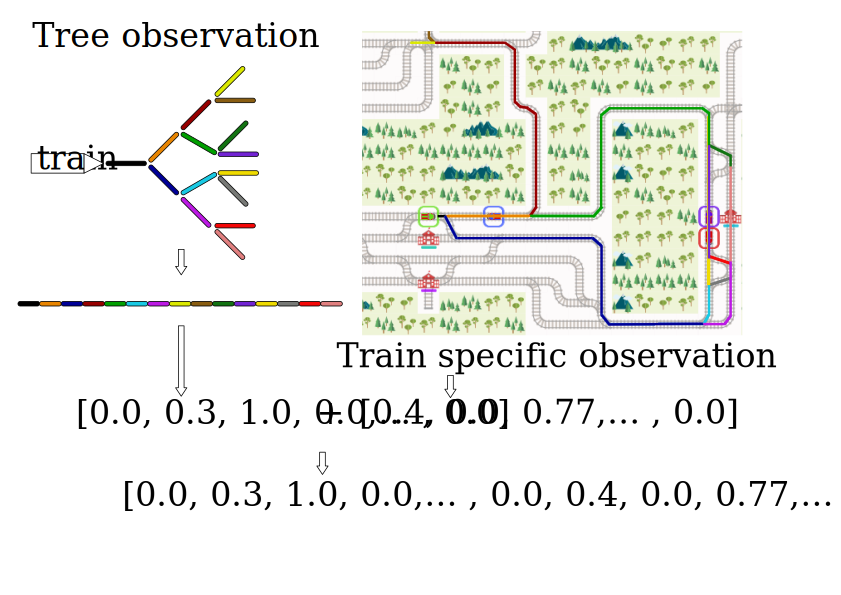
\includegraphics[width=300pt]{diagrams/tree_obs_mapping.pdf}
	\caption{Illustration of the tree observation mapped onto the Flatland enviornment. Each colored bar represents information about a section.}
	\label{fig:obs_descr}
\end{figure}
While this vector already contains all required information outside of the agent, we add another vector with information regarding the agent itself (train specific observation in \autoref{obs_descr}). This vector contains the speed of the agent, the max. speed of the agent, the type of the current tile, the direction the agent is heading and 

\section{Technical Implementation Aspects}\label{software}
In this section, we discuss the most important implementation aspects of our work. 
\subsection*{Used Frameworks and Libraries}\label{framework_and_libraries}
In \autoref{table:used_technologies}, we list the most important used libraries and frameworks in this work.
\begin{table}[H]
	\centering
	\begin{tabularx}{\textwidth}{ |l|c|X| } 
		\hline
		\textbf{Technology}	& \textbf{Version} & \textbf{Description}\\
		\hline
		Python & 3.6 & The whole code for our project is written in Python.\\
		\hline
		Tensorflow & 2.0.0 & Tensorflow provides a framework for both deep learning as well as monitoring the learning process of RL using Tensorboard.\\
		\hline
		MessagegPack & 0.6.2 & MessagePack allows very fast serialization. The resulting binary data is also considerably smaller than serialization with formats like JSON. We use MessagePack to serialize both weights- and gradient-update before sending between worker and model server.\\
		\hline
		Cython & 0.29.14 & Cython allows to compile Python code to natively running C code. We use Cython to speed up our observations on the rail environment.\\
		\hline
		Flask & 1.1.1 & We use Flask as our central model server (see \nameref{dist_architecture}). This Flask application collects gradient updates, distributes the current network weights and allows access to the latest versions of the observation and parameter files.\\
		\hline
		ZLib & (built-in) & ZLib allows to compress in Python. We use ZLib to reduce our payload-size while sending gradient- and weight updates.\\
		\hline
	\end{tabularx}
	\caption{The most important technologies used in this work.}
	\label{table:used_technologies}
\end{table}
\chapter{Experiment Design and Analysis}
\label{chap.experiment}
\chaptermark{Experiments}

\section[Reproducibility]{Reproducibility and Experiment Setup}\label{reproducability}
It is important to note, that the training process of reinforcement learning and especially multi agent reinforcement learning can be hard to reproduce. Depending on the initial weights of the neural networks and the layout of the environments, the performance may vary on each restart. Also in a distributed algorithm, the number of workers can significantly influence the training performance. If not differently specified, we execute all presented experiments on machines with the same specifications (see \autoref{infrastructure}).\\
Another aspect that is hard to reproduce is training stability. In A3C, an important instrument to prevent the policy from converging too early is using an additional entropy term \cite{a3c}. Our way to maintain stability with changing environments is discussed in \autoref{entropy_balancing_hyperparameter}.\\
For better comparability, we try to keep our evaluation versions for the training as similar to each other as possible. If not differently specified, we run evaluations with the following setup:
\begin{itemize}
	\item We use an environment of the size 100x100 tiles with 14 individual agents.
	\item The map contains 20 cities
	\item There is a maximum of 3 rails between cities and a maximum of 4 rails inside cities
	\item Based on the Flatland specification, the maximum allowed number of timesteps is 1608 \cite{flatland_spec}.
\end{itemize}
To analyze the performance of the solution, we run an analyzer that executes 20 rollouts of the environment using the same neural network parameters. After the these 20 rollouts, we update the neural network parameters. For each evaluation round, we use the same 20 environment layouts. 
To compare the performance in a graph, we now take the mean number of agents arrived at their target and plot that in our graph.
\section{Reinforcement Learning for Flatland}
\sectionmark{RL for Flatland}
\label{rl_flatland}
\subsection*{Action Space Reduction and Script Policy Actions}\label{reduced_action_space}
The Flatland environment is designed in a way to resemble a classical RL environment. This means, on every timestep, we receive observations for each agent, calculate an action and hand this action to the environment, visible in pseudocode \autoref{alg:no_reduction}.\\\\
\begin{algorithm}[H]
	\KwData{initialized Flatland environment $\mathcal{E}$, initial observation $\mathcal{s\SPSB{a}{t=0}}$ for all agents }
	\KwResult{terminal Flatland environment}
	initialize buffer $\mathcal{B}$\\
	\While{episode not terminal}{
		create empty action array $\mathcal{A}$\\
		\For{every agent $\mathcal{a}$}{
			get current state $\mathcal{s\SPSB{a}{t}}$ of agent\\
			\textit{// Fetch action for agent, based on current state\\}
			$\mathcal{A[a]} \leftarrow$ from policy $\pi (\mathcal{s\SPSB{a}{t}})$\\
		}
		
		call $\mathcal{env.step(A)}$ \\
		retrieve reward $\mathcal{R}$\\
		append $\mathcal{A}$ to buffer $\mathcal{B}$\\
		retrieve all new states $\mathcal{s_{t+1}}$\\		
	}

	use buffer $\mathcal{B}$ for training of policy $\pi$
	\caption{Default episode for Flatland environment}
	\label{alg:no_reduction}
\end{algorithm}
While this makes sense in an environment where agents need to take an action on every timestep (such as Atari games), in Flatland most of the time the only reasonable action is to move forward as visible in \autoref{fig:no_desicion}. Only around switches, an agent needs to take actions other than just keep going forward.
\begin{figure}[H]
	\centering
	\includegraphics[width=300pt]{images/screenshot_no_decision.png}
	\caption{Screenshot from Flatland environment. A train heading east. The only reasonable action is to ride forward.}
	\label{fig:no_desicion}
\end{figure}
Every action that is produced by the neural network should be included for training, so the network can adapt to this type of situation. The problem arises now, that all these actions of riding forward are included into the training of the agent. The influence of the actions that actually matter (e.g. the ones around switches) is thereby not as big as it could be, because a large portion of the training data is actually situations that do not actually require decisions.\\
To solve this problem, we implement hard coded rules that the agents follow as long as they are not in a situation to make a decision. Only around switches, the neural network policy is activated. As a consequence, the data used for training has less samples but the samples available are of higher quality. The training with this mechanism is shown in \autoref{alg:with_reduction}.
For training, we only use the experience collected near the switch.\\
\begin{algorithm}[H]
	\KwData{initialized Flatland environment $\mathcal{env}$, initial observation $\mathcal{s\SPSB{a}{t=0}}$ for all agents}
	\KwResult{terminal Flatland environment}
	initialize buffer $\mathcal{B}$\\
	\While{episode not terminal}{
		create empty action array $\mathcal{A}$\\
		\For{every agent $\mathcal{a}$}{
			\eIf{agent is near to a switch}{
				get current state $\mathcal{s\SPSB{a}{t}}$ of agent\\
				\textit{// Fetch action for agent, based on current state\\}
				$\mathcal{A[a]} \leftarrow$ from policy $\pi (\mathcal{s\SPSB{a}{t}})$\\
			}{
				$\mathcal{A[a]} \leftarrow \mathcal{u_{forward})}$
			}
		}
		call $\mathcal{env.step(A)}$ \\
		retrieve reward $\mathcal{R}$\\
		\If{agent was near switch}{
			append $\mathcal{s_{t}}$, $\mathcal{A}$ and $\mathcal{R}$ to buffer $\mathcal{B}$\\
		}
		retrieve all new states $\mathcal{s_{t+1}}$\\		
	}
	use buffer $\mathcal{B}$ for training of policy $\pi$\\
	
	\caption{Improved learning algorithm for Flatland environment}
	\label{alg:with_reduction}
\end{algorithm}
This drastically improves training performance as visible in \autoref{chart:action_reduction_comparison}. While both versions have the potential to perform well, based on the observation data, we observe that the version without the action reduction is not able to performe nearly as well as the improved version with reduced actions.
\begin{figure}[H]
	\begin{center}
		%% Creator: Matplotlib, PGF backend
%%
%% To include the figure in your LaTeX document, write
%%   \input{<filename>.pgf}
%%
%% Make sure the required packages are loaded in your preamble
%%   \usepackage{pgf}
%%
%% Figures using additional raster images can only be included by \input if
%% they are in the same directory as the main LaTeX file. For loading figures
%% from other directories you can use the `import` package
%%   \usepackage{import}
%% and then include the figures with
%%   \import{<path to file>}{<filename>.pgf}
%%
%% Matplotlib used the following preamble
%%   \usepackage{fontspec}
%%
\begingroup%
\makeatletter%
\begin{pgfpicture}%
\pgfpathrectangle{\pgfpointorigin}{\pgfqpoint{5.000000in}{3.000000in}}%
\pgfusepath{use as bounding box, clip}%
\begin{pgfscope}%
\pgfsetbuttcap%
\pgfsetmiterjoin%
\definecolor{currentfill}{rgb}{1.000000,1.000000,1.000000}%
\pgfsetfillcolor{currentfill}%
\pgfsetlinewidth{0.000000pt}%
\definecolor{currentstroke}{rgb}{1.000000,1.000000,1.000000}%
\pgfsetstrokecolor{currentstroke}%
\pgfsetdash{}{0pt}%
\pgfpathmoveto{\pgfqpoint{0.000000in}{0.000000in}}%
\pgfpathlineto{\pgfqpoint{5.000000in}{0.000000in}}%
\pgfpathlineto{\pgfqpoint{5.000000in}{3.000000in}}%
\pgfpathlineto{\pgfqpoint{0.000000in}{3.000000in}}%
\pgfpathclose%
\pgfusepath{fill}%
\end{pgfscope}%
\begin{pgfscope}%
\pgfsetbuttcap%
\pgfsetmiterjoin%
\definecolor{currentfill}{rgb}{1.000000,1.000000,1.000000}%
\pgfsetfillcolor{currentfill}%
\pgfsetlinewidth{0.000000pt}%
\definecolor{currentstroke}{rgb}{0.000000,0.000000,0.000000}%
\pgfsetstrokecolor{currentstroke}%
\pgfsetstrokeopacity{0.000000}%
\pgfsetdash{}{0pt}%
\pgfpathmoveto{\pgfqpoint{0.568195in}{0.552638in}}%
\pgfpathlineto{\pgfqpoint{4.848988in}{0.552638in}}%
\pgfpathlineto{\pgfqpoint{4.848988in}{2.837174in}}%
\pgfpathlineto{\pgfqpoint{0.568195in}{2.837174in}}%
\pgfpathclose%
\pgfusepath{fill}%
\end{pgfscope}%
\begin{pgfscope}%
\pgfsetbuttcap%
\pgfsetroundjoin%
\definecolor{currentfill}{rgb}{0.000000,0.000000,0.000000}%
\pgfsetfillcolor{currentfill}%
\pgfsetlinewidth{0.803000pt}%
\definecolor{currentstroke}{rgb}{0.000000,0.000000,0.000000}%
\pgfsetstrokecolor{currentstroke}%
\pgfsetdash{}{0pt}%
\pgfsys@defobject{currentmarker}{\pgfqpoint{0.000000in}{-0.048611in}}{\pgfqpoint{0.000000in}{0.000000in}}{%
\pgfpathmoveto{\pgfqpoint{0.000000in}{0.000000in}}%
\pgfpathlineto{\pgfqpoint{0.000000in}{-0.048611in}}%
\pgfusepath{stroke,fill}%
}%
\begin{pgfscope}%
\pgfsys@transformshift{0.751054in}{0.552638in}%
\pgfsys@useobject{currentmarker}{}%
\end{pgfscope}%
\end{pgfscope}%
\begin{pgfscope}%
\definecolor{textcolor}{rgb}{0.000000,0.000000,0.000000}%
\pgfsetstrokecolor{textcolor}%
\pgfsetfillcolor{textcolor}%
\pgftext[x=0.751054in,y=0.455416in,,top]{\color{textcolor}\rmfamily\fontsize{10.000000}{12.000000}\selectfont \(\displaystyle 0\)}%
\end{pgfscope}%
\begin{pgfscope}%
\pgfsetbuttcap%
\pgfsetroundjoin%
\definecolor{currentfill}{rgb}{0.000000,0.000000,0.000000}%
\pgfsetfillcolor{currentfill}%
\pgfsetlinewidth{0.803000pt}%
\definecolor{currentstroke}{rgb}{0.000000,0.000000,0.000000}%
\pgfsetstrokecolor{currentstroke}%
\pgfsetdash{}{0pt}%
\pgfsys@defobject{currentmarker}{\pgfqpoint{0.000000in}{-0.048611in}}{\pgfqpoint{0.000000in}{0.000000in}}{%
\pgfpathmoveto{\pgfqpoint{0.000000in}{0.000000in}}%
\pgfpathlineto{\pgfqpoint{0.000000in}{-0.048611in}}%
\pgfusepath{stroke,fill}%
}%
\begin{pgfscope}%
\pgfsys@transformshift{1.532506in}{0.552638in}%
\pgfsys@useobject{currentmarker}{}%
\end{pgfscope}%
\end{pgfscope}%
\begin{pgfscope}%
\definecolor{textcolor}{rgb}{0.000000,0.000000,0.000000}%
\pgfsetstrokecolor{textcolor}%
\pgfsetfillcolor{textcolor}%
\pgftext[x=1.532506in,y=0.455416in,,top]{\color{textcolor}\rmfamily\fontsize{10.000000}{12.000000}\selectfont \(\displaystyle 2000\)}%
\end{pgfscope}%
\begin{pgfscope}%
\pgfsetbuttcap%
\pgfsetroundjoin%
\definecolor{currentfill}{rgb}{0.000000,0.000000,0.000000}%
\pgfsetfillcolor{currentfill}%
\pgfsetlinewidth{0.803000pt}%
\definecolor{currentstroke}{rgb}{0.000000,0.000000,0.000000}%
\pgfsetstrokecolor{currentstroke}%
\pgfsetdash{}{0pt}%
\pgfsys@defobject{currentmarker}{\pgfqpoint{0.000000in}{-0.048611in}}{\pgfqpoint{0.000000in}{0.000000in}}{%
\pgfpathmoveto{\pgfqpoint{0.000000in}{0.000000in}}%
\pgfpathlineto{\pgfqpoint{0.000000in}{-0.048611in}}%
\pgfusepath{stroke,fill}%
}%
\begin{pgfscope}%
\pgfsys@transformshift{2.313958in}{0.552638in}%
\pgfsys@useobject{currentmarker}{}%
\end{pgfscope}%
\end{pgfscope}%
\begin{pgfscope}%
\definecolor{textcolor}{rgb}{0.000000,0.000000,0.000000}%
\pgfsetstrokecolor{textcolor}%
\pgfsetfillcolor{textcolor}%
\pgftext[x=2.313958in,y=0.455416in,,top]{\color{textcolor}\rmfamily\fontsize{10.000000}{12.000000}\selectfont \(\displaystyle 4000\)}%
\end{pgfscope}%
\begin{pgfscope}%
\pgfsetbuttcap%
\pgfsetroundjoin%
\definecolor{currentfill}{rgb}{0.000000,0.000000,0.000000}%
\pgfsetfillcolor{currentfill}%
\pgfsetlinewidth{0.803000pt}%
\definecolor{currentstroke}{rgb}{0.000000,0.000000,0.000000}%
\pgfsetstrokecolor{currentstroke}%
\pgfsetdash{}{0pt}%
\pgfsys@defobject{currentmarker}{\pgfqpoint{0.000000in}{-0.048611in}}{\pgfqpoint{0.000000in}{0.000000in}}{%
\pgfpathmoveto{\pgfqpoint{0.000000in}{0.000000in}}%
\pgfpathlineto{\pgfqpoint{0.000000in}{-0.048611in}}%
\pgfusepath{stroke,fill}%
}%
\begin{pgfscope}%
\pgfsys@transformshift{3.095410in}{0.552638in}%
\pgfsys@useobject{currentmarker}{}%
\end{pgfscope}%
\end{pgfscope}%
\begin{pgfscope}%
\definecolor{textcolor}{rgb}{0.000000,0.000000,0.000000}%
\pgfsetstrokecolor{textcolor}%
\pgfsetfillcolor{textcolor}%
\pgftext[x=3.095410in,y=0.455416in,,top]{\color{textcolor}\rmfamily\fontsize{10.000000}{12.000000}\selectfont \(\displaystyle 6000\)}%
\end{pgfscope}%
\begin{pgfscope}%
\pgfsetbuttcap%
\pgfsetroundjoin%
\definecolor{currentfill}{rgb}{0.000000,0.000000,0.000000}%
\pgfsetfillcolor{currentfill}%
\pgfsetlinewidth{0.803000pt}%
\definecolor{currentstroke}{rgb}{0.000000,0.000000,0.000000}%
\pgfsetstrokecolor{currentstroke}%
\pgfsetdash{}{0pt}%
\pgfsys@defobject{currentmarker}{\pgfqpoint{0.000000in}{-0.048611in}}{\pgfqpoint{0.000000in}{0.000000in}}{%
\pgfpathmoveto{\pgfqpoint{0.000000in}{0.000000in}}%
\pgfpathlineto{\pgfqpoint{0.000000in}{-0.048611in}}%
\pgfusepath{stroke,fill}%
}%
\begin{pgfscope}%
\pgfsys@transformshift{3.876862in}{0.552638in}%
\pgfsys@useobject{currentmarker}{}%
\end{pgfscope}%
\end{pgfscope}%
\begin{pgfscope}%
\definecolor{textcolor}{rgb}{0.000000,0.000000,0.000000}%
\pgfsetstrokecolor{textcolor}%
\pgfsetfillcolor{textcolor}%
\pgftext[x=3.876862in,y=0.455416in,,top]{\color{textcolor}\rmfamily\fontsize{10.000000}{12.000000}\selectfont \(\displaystyle 8000\)}%
\end{pgfscope}%
\begin{pgfscope}%
\pgfsetbuttcap%
\pgfsetroundjoin%
\definecolor{currentfill}{rgb}{0.000000,0.000000,0.000000}%
\pgfsetfillcolor{currentfill}%
\pgfsetlinewidth{0.803000pt}%
\definecolor{currentstroke}{rgb}{0.000000,0.000000,0.000000}%
\pgfsetstrokecolor{currentstroke}%
\pgfsetdash{}{0pt}%
\pgfsys@defobject{currentmarker}{\pgfqpoint{0.000000in}{-0.048611in}}{\pgfqpoint{0.000000in}{0.000000in}}{%
\pgfpathmoveto{\pgfqpoint{0.000000in}{0.000000in}}%
\pgfpathlineto{\pgfqpoint{0.000000in}{-0.048611in}}%
\pgfusepath{stroke,fill}%
}%
\begin{pgfscope}%
\pgfsys@transformshift{4.658314in}{0.552638in}%
\pgfsys@useobject{currentmarker}{}%
\end{pgfscope}%
\end{pgfscope}%
\begin{pgfscope}%
\definecolor{textcolor}{rgb}{0.000000,0.000000,0.000000}%
\pgfsetstrokecolor{textcolor}%
\pgfsetfillcolor{textcolor}%
\pgftext[x=4.658314in,y=0.455416in,,top]{\color{textcolor}\rmfamily\fontsize{10.000000}{12.000000}\selectfont \(\displaystyle 10000\)}%
\end{pgfscope}%
\begin{pgfscope}%
\definecolor{textcolor}{rgb}{0.000000,0.000000,0.000000}%
\pgfsetstrokecolor{textcolor}%
\pgfsetfillcolor{textcolor}%
\pgftext[x=2.708591in,y=0.276528in,,top]{\color{textcolor}\rmfamily\fontsize{10.000000}{12.000000}\selectfont Number of training episodes}%
\end{pgfscope}%
\begin{pgfscope}%
\pgfsetbuttcap%
\pgfsetroundjoin%
\definecolor{currentfill}{rgb}{0.000000,0.000000,0.000000}%
\pgfsetfillcolor{currentfill}%
\pgfsetlinewidth{0.803000pt}%
\definecolor{currentstroke}{rgb}{0.000000,0.000000,0.000000}%
\pgfsetstrokecolor{currentstroke}%
\pgfsetdash{}{0pt}%
\pgfsys@defobject{currentmarker}{\pgfqpoint{-0.048611in}{0.000000in}}{\pgfqpoint{0.000000in}{0.000000in}}{%
\pgfpathmoveto{\pgfqpoint{0.000000in}{0.000000in}}%
\pgfpathlineto{\pgfqpoint{-0.048611in}{0.000000in}}%
\pgfusepath{stroke,fill}%
}%
\begin{pgfscope}%
\pgfsys@transformshift{0.568195in}{0.871439in}%
\pgfsys@useobject{currentmarker}{}%
\end{pgfscope}%
\end{pgfscope}%
\begin{pgfscope}%
\definecolor{textcolor}{rgb}{0.000000,0.000000,0.000000}%
\pgfsetstrokecolor{textcolor}%
\pgfsetfillcolor{textcolor}%
\pgftext[x=0.401528in,y=0.823244in,left,base]{\color{textcolor}\rmfamily\fontsize{10.000000}{12.000000}\selectfont \(\displaystyle 2\)}%
\end{pgfscope}%
\begin{pgfscope}%
\pgfsetbuttcap%
\pgfsetroundjoin%
\definecolor{currentfill}{rgb}{0.000000,0.000000,0.000000}%
\pgfsetfillcolor{currentfill}%
\pgfsetlinewidth{0.803000pt}%
\definecolor{currentstroke}{rgb}{0.000000,0.000000,0.000000}%
\pgfsetstrokecolor{currentstroke}%
\pgfsetdash{}{0pt}%
\pgfsys@defobject{currentmarker}{\pgfqpoint{-0.048611in}{0.000000in}}{\pgfqpoint{0.000000in}{0.000000in}}{%
\pgfpathmoveto{\pgfqpoint{0.000000in}{0.000000in}}%
\pgfpathlineto{\pgfqpoint{-0.048611in}{0.000000in}}%
\pgfusepath{stroke,fill}%
}%
\begin{pgfscope}%
\pgfsys@transformshift{0.568195in}{1.257590in}%
\pgfsys@useobject{currentmarker}{}%
\end{pgfscope}%
\end{pgfscope}%
\begin{pgfscope}%
\definecolor{textcolor}{rgb}{0.000000,0.000000,0.000000}%
\pgfsetstrokecolor{textcolor}%
\pgfsetfillcolor{textcolor}%
\pgftext[x=0.401528in,y=1.209396in,left,base]{\color{textcolor}\rmfamily\fontsize{10.000000}{12.000000}\selectfont \(\displaystyle 4\)}%
\end{pgfscope}%
\begin{pgfscope}%
\pgfsetbuttcap%
\pgfsetroundjoin%
\definecolor{currentfill}{rgb}{0.000000,0.000000,0.000000}%
\pgfsetfillcolor{currentfill}%
\pgfsetlinewidth{0.803000pt}%
\definecolor{currentstroke}{rgb}{0.000000,0.000000,0.000000}%
\pgfsetstrokecolor{currentstroke}%
\pgfsetdash{}{0pt}%
\pgfsys@defobject{currentmarker}{\pgfqpoint{-0.048611in}{0.000000in}}{\pgfqpoint{0.000000in}{0.000000in}}{%
\pgfpathmoveto{\pgfqpoint{0.000000in}{0.000000in}}%
\pgfpathlineto{\pgfqpoint{-0.048611in}{0.000000in}}%
\pgfusepath{stroke,fill}%
}%
\begin{pgfscope}%
\pgfsys@transformshift{0.568195in}{1.643741in}%
\pgfsys@useobject{currentmarker}{}%
\end{pgfscope}%
\end{pgfscope}%
\begin{pgfscope}%
\definecolor{textcolor}{rgb}{0.000000,0.000000,0.000000}%
\pgfsetstrokecolor{textcolor}%
\pgfsetfillcolor{textcolor}%
\pgftext[x=0.401528in,y=1.595547in,left,base]{\color{textcolor}\rmfamily\fontsize{10.000000}{12.000000}\selectfont \(\displaystyle 6\)}%
\end{pgfscope}%
\begin{pgfscope}%
\pgfsetbuttcap%
\pgfsetroundjoin%
\definecolor{currentfill}{rgb}{0.000000,0.000000,0.000000}%
\pgfsetfillcolor{currentfill}%
\pgfsetlinewidth{0.803000pt}%
\definecolor{currentstroke}{rgb}{0.000000,0.000000,0.000000}%
\pgfsetstrokecolor{currentstroke}%
\pgfsetdash{}{0pt}%
\pgfsys@defobject{currentmarker}{\pgfqpoint{-0.048611in}{0.000000in}}{\pgfqpoint{0.000000in}{0.000000in}}{%
\pgfpathmoveto{\pgfqpoint{0.000000in}{0.000000in}}%
\pgfpathlineto{\pgfqpoint{-0.048611in}{0.000000in}}%
\pgfusepath{stroke,fill}%
}%
\begin{pgfscope}%
\pgfsys@transformshift{0.568195in}{2.029893in}%
\pgfsys@useobject{currentmarker}{}%
\end{pgfscope}%
\end{pgfscope}%
\begin{pgfscope}%
\definecolor{textcolor}{rgb}{0.000000,0.000000,0.000000}%
\pgfsetstrokecolor{textcolor}%
\pgfsetfillcolor{textcolor}%
\pgftext[x=0.401528in,y=1.981698in,left,base]{\color{textcolor}\rmfamily\fontsize{10.000000}{12.000000}\selectfont \(\displaystyle 8\)}%
\end{pgfscope}%
\begin{pgfscope}%
\pgfsetbuttcap%
\pgfsetroundjoin%
\definecolor{currentfill}{rgb}{0.000000,0.000000,0.000000}%
\pgfsetfillcolor{currentfill}%
\pgfsetlinewidth{0.803000pt}%
\definecolor{currentstroke}{rgb}{0.000000,0.000000,0.000000}%
\pgfsetstrokecolor{currentstroke}%
\pgfsetdash{}{0pt}%
\pgfsys@defobject{currentmarker}{\pgfqpoint{-0.048611in}{0.000000in}}{\pgfqpoint{0.000000in}{0.000000in}}{%
\pgfpathmoveto{\pgfqpoint{0.000000in}{0.000000in}}%
\pgfpathlineto{\pgfqpoint{-0.048611in}{0.000000in}}%
\pgfusepath{stroke,fill}%
}%
\begin{pgfscope}%
\pgfsys@transformshift{0.568195in}{2.416044in}%
\pgfsys@useobject{currentmarker}{}%
\end{pgfscope}%
\end{pgfscope}%
\begin{pgfscope}%
\definecolor{textcolor}{rgb}{0.000000,0.000000,0.000000}%
\pgfsetstrokecolor{textcolor}%
\pgfsetfillcolor{textcolor}%
\pgftext[x=0.332083in,y=2.367850in,left,base]{\color{textcolor}\rmfamily\fontsize{10.000000}{12.000000}\selectfont \(\displaystyle 10\)}%
\end{pgfscope}%
\begin{pgfscope}%
\pgfsetbuttcap%
\pgfsetroundjoin%
\definecolor{currentfill}{rgb}{0.000000,0.000000,0.000000}%
\pgfsetfillcolor{currentfill}%
\pgfsetlinewidth{0.803000pt}%
\definecolor{currentstroke}{rgb}{0.000000,0.000000,0.000000}%
\pgfsetstrokecolor{currentstroke}%
\pgfsetdash{}{0pt}%
\pgfsys@defobject{currentmarker}{\pgfqpoint{-0.048611in}{0.000000in}}{\pgfqpoint{0.000000in}{0.000000in}}{%
\pgfpathmoveto{\pgfqpoint{0.000000in}{0.000000in}}%
\pgfpathlineto{\pgfqpoint{-0.048611in}{0.000000in}}%
\pgfusepath{stroke,fill}%
}%
\begin{pgfscope}%
\pgfsys@transformshift{0.568195in}{2.802195in}%
\pgfsys@useobject{currentmarker}{}%
\end{pgfscope}%
\end{pgfscope}%
\begin{pgfscope}%
\definecolor{textcolor}{rgb}{0.000000,0.000000,0.000000}%
\pgfsetstrokecolor{textcolor}%
\pgfsetfillcolor{textcolor}%
\pgftext[x=0.332083in,y=2.754001in,left,base]{\color{textcolor}\rmfamily\fontsize{10.000000}{12.000000}\selectfont \(\displaystyle 12\)}%
\end{pgfscope}%
\begin{pgfscope}%
\definecolor{textcolor}{rgb}{0.000000,0.000000,0.000000}%
\pgfsetstrokecolor{textcolor}%
\pgfsetfillcolor{textcolor}%
\pgftext[x=0.276528in,y=1.694906in,,bottom,rotate=90.000000]{\color{textcolor}\rmfamily\fontsize{10.000000}{12.000000}\selectfont Number of agents arriving}%
\end{pgfscope}%
\begin{pgfscope}%
\pgfpathrectangle{\pgfqpoint{0.568195in}{0.552638in}}{\pgfqpoint{4.280793in}{2.284536in}}%
\pgfusepath{clip}%
\pgfsetrectcap%
\pgfsetroundjoin%
\pgfsetlinewidth{1.505625pt}%
\definecolor{currentstroke}{rgb}{0.121569,0.466667,0.705882}%
\pgfsetstrokecolor{currentstroke}%
\pgfsetdash{}{0pt}%
\pgfpathmoveto{\pgfqpoint{0.762776in}{0.659678in}}%
\pgfpathlineto{\pgfqpoint{0.782312in}{0.702199in}}%
\pgfpathlineto{\pgfqpoint{0.788173in}{0.673000in}}%
\pgfpathlineto{\pgfqpoint{0.799895in}{0.660986in}}%
\pgfpathlineto{\pgfqpoint{0.831153in}{0.674501in}}%
\pgfpathlineto{\pgfqpoint{0.838968in}{0.665491in}}%
\pgfpathlineto{\pgfqpoint{0.840921in}{0.656481in}}%
\pgfpathlineto{\pgfqpoint{0.844829in}{0.660986in}}%
\pgfpathlineto{\pgfqpoint{0.856550in}{0.679007in}}%
\pgfpathlineto{\pgfqpoint{0.862411in}{0.665491in}}%
\pgfpathlineto{\pgfqpoint{0.879994in}{0.669996in}}%
\pgfpathlineto{\pgfqpoint{0.891716in}{0.660986in}}%
\pgfpathlineto{\pgfqpoint{0.895623in}{0.688017in}}%
\pgfpathlineto{\pgfqpoint{0.897577in}{0.701532in}}%
\pgfpathlineto{\pgfqpoint{0.907345in}{0.710542in}}%
\pgfpathlineto{\pgfqpoint{0.922974in}{0.719552in}}%
\pgfpathlineto{\pgfqpoint{0.936649in}{0.697027in}}%
\pgfpathlineto{\pgfqpoint{0.952278in}{0.751088in}}%
\pgfpathlineto{\pgfqpoint{0.958139in}{0.818665in}}%
\pgfpathlineto{\pgfqpoint{0.960093in}{0.823170in}}%
\pgfpathlineto{\pgfqpoint{0.983536in}{0.868221in}}%
\pgfpathlineto{\pgfqpoint{0.999165in}{0.908767in}}%
\pgfpathlineto{\pgfqpoint{1.006980in}{1.066445in}}%
\pgfpathlineto{\pgfqpoint{1.024562in}{1.552996in}}%
\pgfpathlineto{\pgfqpoint{1.046052in}{1.859342in}}%
\pgfpathlineto{\pgfqpoint{1.055821in}{1.872858in}}%
\pgfpathlineto{\pgfqpoint{1.061681in}{1.899888in}}%
\pgfpathlineto{\pgfqpoint{1.079264in}{1.881868in}}%
\pgfpathlineto{\pgfqpoint{1.081218in}{1.895383in}}%
\pgfpathlineto{\pgfqpoint{1.100754in}{1.917909in}}%
\pgfpathlineto{\pgfqpoint{1.110522in}{1.958455in}}%
\pgfpathlineto{\pgfqpoint{1.114429in}{1.980980in}}%
\pgfpathlineto{\pgfqpoint{1.116383in}{1.999001in}}%
\pgfpathlineto{\pgfqpoint{1.124198in}{1.989990in}}%
\pgfpathlineto{\pgfqpoint{1.139827in}{2.017021in}}%
\pgfpathlineto{\pgfqpoint{1.159363in}{2.242276in}}%
\pgfpathlineto{\pgfqpoint{1.167177in}{2.246781in}}%
\pgfpathlineto{\pgfqpoint{1.188667in}{2.413470in}}%
\pgfpathlineto{\pgfqpoint{1.200389in}{2.404459in}}%
\pgfpathlineto{\pgfqpoint{1.210157in}{2.422480in}}%
\pgfpathlineto{\pgfqpoint{1.216018in}{2.345893in}}%
\pgfpathlineto{\pgfqpoint{1.239462in}{2.233266in}}%
\pgfpathlineto{\pgfqpoint{1.251184in}{2.219750in}}%
\pgfpathlineto{\pgfqpoint{1.260952in}{2.291832in}}%
\pgfpathlineto{\pgfqpoint{1.266813in}{2.345893in}}%
\pgfpathlineto{\pgfqpoint{1.274627in}{2.377429in}}%
\pgfpathlineto{\pgfqpoint{1.282442in}{2.381934in}}%
\pgfpathlineto{\pgfqpoint{1.286349in}{2.372924in}}%
\pgfpathlineto{\pgfqpoint{1.333236in}{2.535107in}}%
\pgfpathlineto{\pgfqpoint{1.335190in}{2.530602in}}%
\pgfpathlineto{\pgfqpoint{1.344958in}{2.454016in}}%
\pgfpathlineto{\pgfqpoint{1.354726in}{2.422480in}}%
\pgfpathlineto{\pgfqpoint{1.358633in}{2.458521in}}%
\pgfpathlineto{\pgfqpoint{1.374262in}{2.499067in}}%
\pgfpathlineto{\pgfqpoint{1.376216in}{2.539612in}}%
\pgfpathlineto{\pgfqpoint{1.387938in}{2.584663in}}%
\pgfpathlineto{\pgfqpoint{1.391845in}{2.539612in}}%
\pgfpathlineto{\pgfqpoint{1.397706in}{2.530602in}}%
\pgfpathlineto{\pgfqpoint{1.415288in}{2.336883in}}%
\pgfpathlineto{\pgfqpoint{1.430917in}{2.386439in}}%
\pgfpathlineto{\pgfqpoint{1.462176in}{2.440500in}}%
\pgfpathlineto{\pgfqpoint{1.469990in}{2.381934in}}%
\pgfpathlineto{\pgfqpoint{1.481712in}{2.408965in}}%
\pgfpathlineto{\pgfqpoint{1.489526in}{2.449511in}}%
\pgfpathlineto{\pgfqpoint{1.493434in}{2.503572in}}%
\pgfpathlineto{\pgfqpoint{1.516877in}{2.426985in}}%
\pgfpathlineto{\pgfqpoint{1.518831in}{2.435995in}}%
\pgfpathlineto{\pgfqpoint{1.550089in}{2.449511in}}%
\pgfpathlineto{\pgfqpoint{1.575486in}{2.454016in}}%
\pgfpathlineto{\pgfqpoint{1.577440in}{2.463026in}}%
\pgfpathlineto{\pgfqpoint{1.581347in}{2.458521in}}%
\pgfpathlineto{\pgfqpoint{1.593069in}{2.517087in}}%
\pgfpathlineto{\pgfqpoint{1.610651in}{2.571148in}}%
\pgfpathlineto{\pgfqpoint{1.614559in}{2.539612in}}%
\pgfpathlineto{\pgfqpoint{1.616512in}{2.503572in}}%
\pgfpathlineto{\pgfqpoint{1.622373in}{2.481046in}}%
\pgfpathlineto{\pgfqpoint{1.634095in}{2.399954in}}%
\pgfpathlineto{\pgfqpoint{1.651678in}{2.417975in}}%
\pgfpathlineto{\pgfqpoint{1.657538in}{2.440500in}}%
\pgfpathlineto{\pgfqpoint{1.659492in}{2.422480in}}%
\pgfpathlineto{\pgfqpoint{1.677075in}{2.440500in}}%
\pgfpathlineto{\pgfqpoint{1.679028in}{2.445005in}}%
\pgfpathlineto{\pgfqpoint{1.708333in}{2.341388in}}%
\pgfpathlineto{\pgfqpoint{1.712240in}{2.381934in}}%
\pgfpathlineto{\pgfqpoint{1.716147in}{2.332378in}}%
\pgfpathlineto{\pgfqpoint{1.753266in}{2.508077in}}%
\pgfpathlineto{\pgfqpoint{1.757174in}{2.562138in}}%
\pgfpathlineto{\pgfqpoint{1.763034in}{2.620704in}}%
\pgfpathlineto{\pgfqpoint{1.778664in}{2.580158in}}%
\pgfpathlineto{\pgfqpoint{1.790385in}{2.598179in}}%
\pgfpathlineto{\pgfqpoint{1.794293in}{2.580158in}}%
\pgfpathlineto{\pgfqpoint{1.800153in}{2.472036in}}%
\pgfpathlineto{\pgfqpoint{1.811875in}{2.494562in}}%
\pgfpathlineto{\pgfqpoint{1.821643in}{2.499067in}}%
\pgfpathlineto{\pgfqpoint{1.841180in}{2.422480in}}%
\pgfpathlineto{\pgfqpoint{1.845087in}{2.499067in}}%
\pgfpathlineto{\pgfqpoint{1.852901in}{2.408965in}}%
\pgfpathlineto{\pgfqpoint{1.864623in}{2.390944in}}%
\pgfpathlineto{\pgfqpoint{1.872438in}{2.323368in}}%
\pgfpathlineto{\pgfqpoint{1.874391in}{2.323368in}}%
\pgfpathlineto{\pgfqpoint{1.884160in}{2.354903in}}%
\pgfpathlineto{\pgfqpoint{1.888067in}{2.323368in}}%
\pgfpathlineto{\pgfqpoint{1.890020in}{2.386439in}}%
\pgfpathlineto{\pgfqpoint{1.893928in}{2.381934in}}%
\pgfpathlineto{\pgfqpoint{1.899789in}{2.359409in}}%
\pgfpathlineto{\pgfqpoint{1.909557in}{2.390944in}}%
\pgfpathlineto{\pgfqpoint{1.911510in}{2.463026in}}%
\pgfpathlineto{\pgfqpoint{1.929093in}{2.467531in}}%
\pgfpathlineto{\pgfqpoint{1.940815in}{2.431490in}}%
\pgfpathlineto{\pgfqpoint{1.944722in}{2.454016in}}%
\pgfpathlineto{\pgfqpoint{1.954490in}{2.454016in}}%
\pgfpathlineto{\pgfqpoint{1.964258in}{2.476541in}}%
\pgfpathlineto{\pgfqpoint{1.968166in}{2.494562in}}%
\pgfpathlineto{\pgfqpoint{1.991609in}{2.485551in}}%
\pgfpathlineto{\pgfqpoint{2.005285in}{2.512582in}}%
\pgfpathlineto{\pgfqpoint{2.007238in}{2.521592in}}%
\pgfpathlineto{\pgfqpoint{2.015053in}{2.584663in}}%
\pgfpathlineto{\pgfqpoint{2.017006in}{2.539612in}}%
\pgfpathlineto{\pgfqpoint{2.020914in}{2.562138in}}%
\pgfpathlineto{\pgfqpoint{2.026774in}{2.634220in}}%
\pgfpathlineto{\pgfqpoint{2.034589in}{2.562138in}}%
\pgfpathlineto{\pgfqpoint{2.044357in}{2.530602in}}%
\pgfpathlineto{\pgfqpoint{2.050218in}{2.494562in}}%
\pgfpathlineto{\pgfqpoint{2.058033in}{2.503572in}}%
\pgfpathlineto{\pgfqpoint{2.063893in}{2.458521in}}%
\pgfpathlineto{\pgfqpoint{2.069754in}{2.490056in}}%
\pgfpathlineto{\pgfqpoint{2.077569in}{2.539612in}}%
\pgfpathlineto{\pgfqpoint{2.079522in}{2.526097in}}%
\pgfpathlineto{\pgfqpoint{2.087337in}{2.584663in}}%
\pgfpathlineto{\pgfqpoint{2.097105in}{2.566643in}}%
\pgfpathlineto{\pgfqpoint{2.099059in}{2.580158in}}%
\pgfpathlineto{\pgfqpoint{2.112734in}{2.548623in}}%
\pgfpathlineto{\pgfqpoint{2.126410in}{2.481046in}}%
\pgfpathlineto{\pgfqpoint{2.132270in}{2.508077in}}%
\pgfpathlineto{\pgfqpoint{2.147899in}{2.508077in}}%
\pgfpathlineto{\pgfqpoint{2.155714in}{2.557633in}}%
\pgfpathlineto{\pgfqpoint{2.161575in}{2.602684in}}%
\pgfpathlineto{\pgfqpoint{2.165482in}{2.566643in}}%
\pgfpathlineto{\pgfqpoint{2.179158in}{2.566643in}}%
\pgfpathlineto{\pgfqpoint{2.190879in}{2.544118in}}%
\pgfpathlineto{\pgfqpoint{2.194787in}{2.571148in}}%
\pgfpathlineto{\pgfqpoint{2.196740in}{2.575653in}}%
\pgfpathlineto{\pgfqpoint{2.204555in}{2.611694in}}%
\pgfpathlineto{\pgfqpoint{2.212369in}{2.571148in}}%
\pgfpathlineto{\pgfqpoint{2.220184in}{2.589169in}}%
\pgfpathlineto{\pgfqpoint{2.222137in}{2.575653in}}%
\pgfpathlineto{\pgfqpoint{2.229952in}{2.575653in}}%
\pgfpathlineto{\pgfqpoint{2.247535in}{2.553128in}}%
\pgfpathlineto{\pgfqpoint{2.255349in}{2.530602in}}%
\pgfpathlineto{\pgfqpoint{2.257303in}{2.553128in}}%
\pgfpathlineto{\pgfqpoint{2.259256in}{2.548623in}}%
\pgfpathlineto{\pgfqpoint{2.263164in}{2.548623in}}%
\pgfpathlineto{\pgfqpoint{2.265117in}{2.553128in}}%
\pgfpathlineto{\pgfqpoint{2.276839in}{2.508077in}}%
\pgfpathlineto{\pgfqpoint{2.284654in}{2.526097in}}%
\pgfpathlineto{\pgfqpoint{2.286607in}{2.539612in}}%
\pgfpathlineto{\pgfqpoint{2.290514in}{2.535107in}}%
\pgfpathlineto{\pgfqpoint{2.294422in}{2.593674in}}%
\pgfpathlineto{\pgfqpoint{2.300283in}{2.598179in}}%
\pgfpathlineto{\pgfqpoint{2.302236in}{2.611694in}}%
\pgfpathlineto{\pgfqpoint{2.306143in}{2.593674in}}%
\pgfpathlineto{\pgfqpoint{2.312004in}{2.593674in}}%
\pgfpathlineto{\pgfqpoint{2.319819in}{2.602684in}}%
\pgfpathlineto{\pgfqpoint{2.329587in}{2.611694in}}%
\pgfpathlineto{\pgfqpoint{2.331541in}{2.584663in}}%
\pgfpathlineto{\pgfqpoint{2.333494in}{2.593674in}}%
\pgfpathlineto{\pgfqpoint{2.345216in}{2.580158in}}%
\pgfpathlineto{\pgfqpoint{2.356938in}{2.625209in}}%
\pgfpathlineto{\pgfqpoint{2.364752in}{2.620704in}}%
\pgfpathlineto{\pgfqpoint{2.370613in}{2.638725in}}%
\pgfpathlineto{\pgfqpoint{2.378428in}{2.580158in}}%
\pgfpathlineto{\pgfqpoint{2.386242in}{2.562138in}}%
\pgfpathlineto{\pgfqpoint{2.390150in}{2.580158in}}%
\pgfpathlineto{\pgfqpoint{2.399918in}{2.517087in}}%
\pgfpathlineto{\pgfqpoint{2.446805in}{2.548623in}}%
\pgfpathlineto{\pgfqpoint{2.450712in}{2.584663in}}%
\pgfpathlineto{\pgfqpoint{2.452666in}{2.562138in}}%
\pgfpathlineto{\pgfqpoint{2.460480in}{2.535107in}}%
\pgfpathlineto{\pgfqpoint{2.464387in}{2.530602in}}%
\pgfpathlineto{\pgfqpoint{2.472202in}{2.517087in}}%
\pgfpathlineto{\pgfqpoint{2.476109in}{2.512582in}}%
\pgfpathlineto{\pgfqpoint{2.491738in}{2.472036in}}%
\pgfpathlineto{\pgfqpoint{2.503460in}{2.521592in}}%
\pgfpathlineto{\pgfqpoint{2.511275in}{2.539612in}}%
\pgfpathlineto{\pgfqpoint{2.524950in}{2.539612in}}%
\pgfpathlineto{\pgfqpoint{2.526904in}{2.548623in}}%
\pgfpathlineto{\pgfqpoint{2.528857in}{2.526097in}}%
\pgfpathlineto{\pgfqpoint{2.530811in}{2.521592in}}%
\pgfpathlineto{\pgfqpoint{2.540579in}{2.593674in}}%
\pgfpathlineto{\pgfqpoint{2.544486in}{2.611694in}}%
\pgfpathlineto{\pgfqpoint{2.550347in}{2.575653in}}%
\pgfpathlineto{\pgfqpoint{2.552301in}{2.575653in}}%
\pgfpathlineto{\pgfqpoint{2.556208in}{2.589169in}}%
\pgfpathlineto{\pgfqpoint{2.571837in}{2.557633in}}%
\pgfpathlineto{\pgfqpoint{2.573791in}{2.580158in}}%
\pgfpathlineto{\pgfqpoint{2.579652in}{2.544118in}}%
\pgfpathlineto{\pgfqpoint{2.593327in}{2.566643in}}%
\pgfpathlineto{\pgfqpoint{2.599188in}{2.508077in}}%
\pgfpathlineto{\pgfqpoint{2.616771in}{2.625209in}}%
\pgfpathlineto{\pgfqpoint{2.620678in}{2.598179in}}%
\pgfpathlineto{\pgfqpoint{2.624585in}{2.589169in}}%
\pgfpathlineto{\pgfqpoint{2.630446in}{2.593674in}}%
\pgfpathlineto{\pgfqpoint{2.632400in}{2.575653in}}%
\pgfpathlineto{\pgfqpoint{2.640214in}{2.665755in}}%
\pgfpathlineto{\pgfqpoint{2.649982in}{2.688281in}}%
\pgfpathlineto{\pgfqpoint{2.651936in}{2.683776in}}%
\pgfpathlineto{\pgfqpoint{2.659750in}{2.656745in}}%
\pgfpathlineto{\pgfqpoint{2.661704in}{2.643230in}}%
\pgfpathlineto{\pgfqpoint{2.663658in}{2.647735in}}%
\pgfpathlineto{\pgfqpoint{2.665611in}{2.625209in}}%
\pgfpathlineto{\pgfqpoint{2.675379in}{2.584663in}}%
\pgfpathlineto{\pgfqpoint{2.681240in}{2.535107in}}%
\pgfpathlineto{\pgfqpoint{2.683194in}{2.535107in}}%
\pgfpathlineto{\pgfqpoint{2.698823in}{2.544118in}}%
\pgfpathlineto{\pgfqpoint{2.710545in}{2.449511in}}%
\pgfpathlineto{\pgfqpoint{2.714452in}{2.445005in}}%
\pgfpathlineto{\pgfqpoint{2.716406in}{2.404459in}}%
\pgfpathlineto{\pgfqpoint{2.732035in}{2.422480in}}%
\pgfpathlineto{\pgfqpoint{2.733988in}{2.413470in}}%
\pgfpathlineto{\pgfqpoint{2.739849in}{2.422480in}}%
\pgfpathlineto{\pgfqpoint{2.755478in}{2.544118in}}%
\pgfpathlineto{\pgfqpoint{2.759386in}{2.512582in}}%
\pgfpathlineto{\pgfqpoint{2.767200in}{2.494562in}}%
\pgfpathlineto{\pgfqpoint{2.769154in}{2.521592in}}%
\pgfpathlineto{\pgfqpoint{2.778922in}{2.580158in}}%
\pgfpathlineto{\pgfqpoint{2.792597in}{2.580158in}}%
\pgfpathlineto{\pgfqpoint{2.814087in}{2.607189in}}%
\pgfpathlineto{\pgfqpoint{2.817994in}{2.535107in}}%
\pgfpathlineto{\pgfqpoint{2.829716in}{2.589169in}}%
\pgfpathlineto{\pgfqpoint{2.835577in}{2.584663in}}%
\pgfpathlineto{\pgfqpoint{2.839484in}{2.616199in}}%
\pgfpathlineto{\pgfqpoint{2.847299in}{2.611694in}}%
\pgfpathlineto{\pgfqpoint{2.855113in}{2.571148in}}%
\pgfpathlineto{\pgfqpoint{2.859021in}{2.562138in}}%
\pgfpathlineto{\pgfqpoint{2.868789in}{2.548623in}}%
\pgfpathlineto{\pgfqpoint{2.870742in}{2.535107in}}%
\pgfpathlineto{\pgfqpoint{2.872696in}{2.580158in}}%
\pgfpathlineto{\pgfqpoint{2.888325in}{2.544118in}}%
\pgfpathlineto{\pgfqpoint{2.900047in}{2.616199in}}%
\pgfpathlineto{\pgfqpoint{2.909815in}{2.638725in}}%
\pgfpathlineto{\pgfqpoint{2.911769in}{2.625209in}}%
\pgfpathlineto{\pgfqpoint{2.929351in}{2.593674in}}%
\pgfpathlineto{\pgfqpoint{2.939119in}{2.557633in}}%
\pgfpathlineto{\pgfqpoint{2.950841in}{2.445005in}}%
\pgfpathlineto{\pgfqpoint{2.966470in}{2.463026in}}%
\pgfpathlineto{\pgfqpoint{2.970378in}{2.481046in}}%
\pgfpathlineto{\pgfqpoint{3.009450in}{2.566643in}}%
\pgfpathlineto{\pgfqpoint{3.011404in}{2.508077in}}%
\pgfpathlineto{\pgfqpoint{3.019218in}{2.481046in}}%
\pgfpathlineto{\pgfqpoint{3.021172in}{2.544118in}}%
\pgfpathlineto{\pgfqpoint{3.023126in}{2.553128in}}%
\pgfpathlineto{\pgfqpoint{3.058291in}{2.481046in}}%
\pgfpathlineto{\pgfqpoint{3.068059in}{2.494562in}}%
\pgfpathlineto{\pgfqpoint{3.081734in}{2.472036in}}%
\pgfpathlineto{\pgfqpoint{3.083688in}{2.463026in}}%
\pgfpathlineto{\pgfqpoint{3.095410in}{2.481046in}}%
\pgfpathlineto{\pgfqpoint{3.099317in}{2.530602in}}%
\pgfpathlineto{\pgfqpoint{3.109085in}{2.472036in}}%
\pgfpathlineto{\pgfqpoint{3.112993in}{2.490056in}}%
\pgfpathlineto{\pgfqpoint{3.124714in}{2.566643in}}%
\pgfpathlineto{\pgfqpoint{3.159880in}{2.697291in}}%
\pgfpathlineto{\pgfqpoint{3.163787in}{2.683776in}}%
\pgfpathlineto{\pgfqpoint{3.167694in}{2.733332in}}%
\pgfpathlineto{\pgfqpoint{3.183323in}{2.692786in}}%
\pgfpathlineto{\pgfqpoint{3.189184in}{2.683776in}}%
\pgfpathlineto{\pgfqpoint{3.200906in}{2.575653in}}%
\pgfpathlineto{\pgfqpoint{3.204813in}{2.557633in}}%
\pgfpathlineto{\pgfqpoint{3.208720in}{2.548623in}}%
\pgfpathlineto{\pgfqpoint{3.210674in}{2.530602in}}%
\pgfpathlineto{\pgfqpoint{3.216535in}{2.544118in}}%
\pgfpathlineto{\pgfqpoint{3.226303in}{2.508077in}}%
\pgfpathlineto{\pgfqpoint{3.241932in}{2.593674in}}%
\pgfpathlineto{\pgfqpoint{3.255607in}{2.593674in}}%
\pgfpathlineto{\pgfqpoint{3.267329in}{2.616199in}}%
\pgfpathlineto{\pgfqpoint{3.275144in}{2.616199in}}%
\pgfpathlineto{\pgfqpoint{3.279051in}{2.580158in}}%
\pgfpathlineto{\pgfqpoint{3.281005in}{2.607189in}}%
\pgfpathlineto{\pgfqpoint{3.292726in}{2.557633in}}%
\pgfpathlineto{\pgfqpoint{3.312263in}{2.620704in}}%
\pgfpathlineto{\pgfqpoint{3.316170in}{2.611694in}}%
\pgfpathlineto{\pgfqpoint{3.322031in}{2.521592in}}%
\pgfpathlineto{\pgfqpoint{3.323985in}{2.530602in}}%
\pgfpathlineto{\pgfqpoint{3.329845in}{2.571148in}}%
\pgfpathlineto{\pgfqpoint{3.341567in}{2.553128in}}%
\pgfpathlineto{\pgfqpoint{3.351335in}{2.440500in}}%
\pgfpathlineto{\pgfqpoint{3.357196in}{2.458521in}}%
\pgfpathlineto{\pgfqpoint{3.363057in}{2.530602in}}%
\pgfpathlineto{\pgfqpoint{3.365011in}{2.539612in}}%
\pgfpathlineto{\pgfqpoint{3.400176in}{2.526097in}}%
\pgfpathlineto{\pgfqpoint{3.421666in}{2.553128in}}%
\pgfpathlineto{\pgfqpoint{3.429481in}{2.575653in}}%
\pgfpathlineto{\pgfqpoint{3.458785in}{2.562138in}}%
\pgfpathlineto{\pgfqpoint{3.464646in}{2.544118in}}%
\pgfpathlineto{\pgfqpoint{3.466599in}{2.544118in}}%
\pgfpathlineto{\pgfqpoint{3.472460in}{2.494562in}}%
\pgfpathlineto{\pgfqpoint{3.513487in}{2.508077in}}%
\pgfpathlineto{\pgfqpoint{3.515440in}{2.494562in}}%
\pgfpathlineto{\pgfqpoint{3.525208in}{2.481046in}}%
\pgfpathlineto{\pgfqpoint{3.531069in}{2.490056in}}%
\pgfpathlineto{\pgfqpoint{3.538884in}{2.593674in}}%
\pgfpathlineto{\pgfqpoint{3.542791in}{2.562138in}}%
\pgfpathlineto{\pgfqpoint{3.550606in}{2.566643in}}%
\pgfpathlineto{\pgfqpoint{3.558420in}{2.512582in}}%
\pgfpathlineto{\pgfqpoint{3.566235in}{2.557633in}}%
\pgfpathlineto{\pgfqpoint{3.597493in}{2.611694in}}%
\pgfpathlineto{\pgfqpoint{3.617029in}{2.530602in}}%
\pgfpathlineto{\pgfqpoint{3.638519in}{2.454016in}}%
\pgfpathlineto{\pgfqpoint{3.654148in}{2.490056in}}%
\pgfpathlineto{\pgfqpoint{3.656102in}{2.503572in}}%
\pgfpathlineto{\pgfqpoint{3.661962in}{2.467531in}}%
\pgfpathlineto{\pgfqpoint{3.665870in}{2.499067in}}%
\pgfpathlineto{\pgfqpoint{3.667823in}{2.530602in}}%
\pgfpathlineto{\pgfqpoint{3.683452in}{2.499067in}}%
\pgfpathlineto{\pgfqpoint{3.685406in}{2.503572in}}%
\pgfpathlineto{\pgfqpoint{3.699081in}{2.530602in}}%
\pgfpathlineto{\pgfqpoint{3.702989in}{2.503572in}}%
\pgfpathlineto{\pgfqpoint{3.718618in}{2.485551in}}%
\pgfpathlineto{\pgfqpoint{3.728386in}{2.508077in}}%
\pgfpathlineto{\pgfqpoint{3.730339in}{2.530602in}}%
\pgfpathlineto{\pgfqpoint{3.736200in}{2.512582in}}%
\pgfpathlineto{\pgfqpoint{3.749876in}{2.602684in}}%
\pgfpathlineto{\pgfqpoint{3.773319in}{2.521592in}}%
\pgfpathlineto{\pgfqpoint{3.783087in}{2.535107in}}%
\pgfpathlineto{\pgfqpoint{3.785041in}{2.517087in}}%
\pgfpathlineto{\pgfqpoint{3.788948in}{2.521592in}}%
\pgfpathlineto{\pgfqpoint{3.802624in}{2.544118in}}%
\pgfpathlineto{\pgfqpoint{3.816299in}{2.521592in}}%
\pgfpathlineto{\pgfqpoint{3.818253in}{2.499067in}}%
\pgfpathlineto{\pgfqpoint{3.835835in}{2.490056in}}%
\pgfpathlineto{\pgfqpoint{3.843650in}{2.517087in}}%
\pgfpathlineto{\pgfqpoint{3.847557in}{2.539612in}}%
\pgfpathlineto{\pgfqpoint{3.855372in}{2.503572in}}%
\pgfpathlineto{\pgfqpoint{3.872954in}{2.512582in}}%
\pgfpathlineto{\pgfqpoint{3.886630in}{2.521592in}}%
\pgfpathlineto{\pgfqpoint{3.888583in}{2.548623in}}%
\pgfpathlineto{\pgfqpoint{3.898352in}{2.530602in}}%
\pgfpathlineto{\pgfqpoint{3.913981in}{2.616199in}}%
\pgfpathlineto{\pgfqpoint{3.917888in}{2.616199in}}%
\pgfpathlineto{\pgfqpoint{3.931563in}{2.593674in}}%
\pgfpathlineto{\pgfqpoint{3.933517in}{2.620704in}}%
\pgfpathlineto{\pgfqpoint{3.941331in}{2.634220in}}%
\pgfpathlineto{\pgfqpoint{3.951100in}{2.535107in}}%
\pgfpathlineto{\pgfqpoint{3.956961in}{2.530602in}}%
\pgfpathlineto{\pgfqpoint{3.960868in}{2.544118in}}%
\pgfpathlineto{\pgfqpoint{3.966729in}{2.503572in}}%
\pgfpathlineto{\pgfqpoint{3.972590in}{2.499067in}}%
\pgfpathlineto{\pgfqpoint{3.980404in}{2.449511in}}%
\pgfpathlineto{\pgfqpoint{3.996033in}{2.435995in}}%
\pgfpathlineto{\pgfqpoint{4.011662in}{2.499067in}}%
\pgfpathlineto{\pgfqpoint{4.019477in}{2.557633in}}%
\pgfpathlineto{\pgfqpoint{4.025338in}{2.562138in}}%
\pgfpathlineto{\pgfqpoint{4.027291in}{2.544118in}}%
\pgfpathlineto{\pgfqpoint{4.040967in}{2.611694in}}%
\pgfpathlineto{\pgfqpoint{4.056596in}{2.697291in}}%
\pgfpathlineto{\pgfqpoint{4.064410in}{2.697291in}}%
\pgfpathlineto{\pgfqpoint{4.066364in}{2.706301in}}%
\pgfpathlineto{\pgfqpoint{4.068317in}{2.724322in}}%
\pgfpathlineto{\pgfqpoint{4.072225in}{2.656745in}}%
\pgfpathlineto{\pgfqpoint{4.078086in}{2.674765in}}%
\pgfpathlineto{\pgfqpoint{4.093715in}{2.575653in}}%
\pgfpathlineto{\pgfqpoint{4.107390in}{2.530602in}}%
\pgfpathlineto{\pgfqpoint{4.111297in}{2.580158in}}%
\pgfpathlineto{\pgfqpoint{4.128880in}{2.580158in}}%
\pgfpathlineto{\pgfqpoint{4.136694in}{2.562138in}}%
\pgfpathlineto{\pgfqpoint{4.140602in}{2.593674in}}%
\pgfpathlineto{\pgfqpoint{4.142555in}{2.593674in}}%
\pgfpathlineto{\pgfqpoint{4.146463in}{2.589169in}}%
\pgfpathlineto{\pgfqpoint{4.156231in}{2.566643in}}%
\pgfpathlineto{\pgfqpoint{4.158184in}{2.535107in}}%
\pgfpathlineto{\pgfqpoint{4.162092in}{2.512582in}}%
\pgfpathlineto{\pgfqpoint{4.164045in}{2.530602in}}%
\pgfpathlineto{\pgfqpoint{4.165999in}{2.512582in}}%
\pgfpathlineto{\pgfqpoint{4.175767in}{2.499067in}}%
\pgfpathlineto{\pgfqpoint{4.203118in}{2.499067in}}%
\pgfpathlineto{\pgfqpoint{4.220701in}{2.566643in}}%
\pgfpathlineto{\pgfqpoint{4.232422in}{2.607189in}}%
\pgfpathlineto{\pgfqpoint{4.246098in}{2.557633in}}%
\pgfpathlineto{\pgfqpoint{4.248051in}{2.571148in}}%
\pgfpathlineto{\pgfqpoint{4.265634in}{2.530602in}}%
\pgfpathlineto{\pgfqpoint{4.279309in}{2.562138in}}%
\pgfpathlineto{\pgfqpoint{4.296892in}{2.472036in}}%
\pgfpathlineto{\pgfqpoint{4.302753in}{2.494562in}}%
\pgfpathlineto{\pgfqpoint{4.316428in}{2.508077in}}%
\pgfpathlineto{\pgfqpoint{4.320336in}{2.530602in}}%
\pgfpathlineto{\pgfqpoint{4.328150in}{2.584663in}}%
\pgfpathlineto{\pgfqpoint{4.347686in}{2.508077in}}%
\pgfpathlineto{\pgfqpoint{4.349640in}{2.521592in}}%
\pgfpathlineto{\pgfqpoint{4.355501in}{2.526097in}}%
\pgfpathlineto{\pgfqpoint{4.365269in}{2.458521in}}%
\pgfpathlineto{\pgfqpoint{4.373084in}{2.539612in}}%
\pgfpathlineto{\pgfqpoint{4.398481in}{2.539612in}}%
\pgfpathlineto{\pgfqpoint{4.402388in}{2.517087in}}%
\pgfpathlineto{\pgfqpoint{4.404342in}{2.499067in}}%
\pgfpathlineto{\pgfqpoint{4.416063in}{2.503572in}}%
\pgfpathlineto{\pgfqpoint{4.418017in}{2.485551in}}%
\pgfpathlineto{\pgfqpoint{4.419971in}{2.494562in}}%
\pgfpathlineto{\pgfqpoint{4.423878in}{2.521592in}}%
\pgfpathlineto{\pgfqpoint{4.427785in}{2.557633in}}%
\pgfpathlineto{\pgfqpoint{4.451229in}{2.656745in}}%
\pgfpathlineto{\pgfqpoint{4.486394in}{2.571148in}}%
\pgfpathlineto{\pgfqpoint{4.498116in}{2.598179in}}%
\pgfpathlineto{\pgfqpoint{4.509838in}{2.557633in}}%
\pgfpathlineto{\pgfqpoint{4.511791in}{2.566643in}}%
\pgfpathlineto{\pgfqpoint{4.523513in}{2.607189in}}%
\pgfpathlineto{\pgfqpoint{4.531328in}{2.562138in}}%
\pgfpathlineto{\pgfqpoint{4.535235in}{2.557633in}}%
\pgfpathlineto{\pgfqpoint{4.539142in}{2.508077in}}%
\pgfpathlineto{\pgfqpoint{4.550864in}{2.526097in}}%
\pgfpathlineto{\pgfqpoint{4.556725in}{2.472036in}}%
\pgfpathlineto{\pgfqpoint{4.560632in}{2.458521in}}%
\pgfpathlineto{\pgfqpoint{4.566493in}{2.449511in}}%
\pgfpathlineto{\pgfqpoint{4.572354in}{2.449511in}}%
\pgfpathlineto{\pgfqpoint{4.578215in}{2.530602in}}%
\pgfpathlineto{\pgfqpoint{4.595797in}{2.566643in}}%
\pgfpathlineto{\pgfqpoint{4.599705in}{2.580158in}}%
\pgfpathlineto{\pgfqpoint{4.623148in}{2.634220in}}%
\pgfpathlineto{\pgfqpoint{4.625102in}{2.625209in}}%
\pgfpathlineto{\pgfqpoint{4.627055in}{2.607189in}}%
\pgfpathlineto{\pgfqpoint{4.654406in}{2.445005in}}%
\pgfpathlineto{\pgfqpoint{4.654406in}{2.445005in}}%
\pgfusepath{stroke}%
\end{pgfscope}%
\begin{pgfscope}%
\pgfpathrectangle{\pgfqpoint{0.568195in}{0.552638in}}{\pgfqpoint{4.280793in}{2.284536in}}%
\pgfusepath{clip}%
\pgfsetrectcap%
\pgfsetroundjoin%
\pgfsetlinewidth{1.505625pt}%
\definecolor{currentstroke}{rgb}{1.000000,0.498039,0.054902}%
\pgfsetstrokecolor{currentstroke}%
\pgfsetdash{}{0pt}%
\pgfpathmoveto{\pgfqpoint{0.762776in}{0.906732in}}%
\pgfpathlineto{\pgfqpoint{0.788173in}{0.921719in}}%
\pgfpathlineto{\pgfqpoint{0.799895in}{0.935797in}}%
\pgfpathlineto{\pgfqpoint{0.835060in}{1.116001in}}%
\pgfpathlineto{\pgfqpoint{0.840921in}{1.174567in}}%
\pgfpathlineto{\pgfqpoint{0.856550in}{1.224124in}}%
\pgfpathlineto{\pgfqpoint{0.862411in}{1.215113in}}%
\pgfpathlineto{\pgfqpoint{0.891716in}{1.278185in}}%
\pgfpathlineto{\pgfqpoint{0.897577in}{1.287195in}}%
\pgfpathlineto{\pgfqpoint{0.936649in}{1.543986in}}%
\pgfpathlineto{\pgfqpoint{0.952278in}{1.525965in}}%
\pgfpathlineto{\pgfqpoint{0.960093in}{1.521460in}}%
\pgfpathlineto{\pgfqpoint{0.999165in}{1.485419in}}%
\pgfpathlineto{\pgfqpoint{1.024562in}{1.503440in}}%
\pgfpathlineto{\pgfqpoint{1.046052in}{1.467399in}}%
\pgfpathlineto{\pgfqpoint{1.055821in}{1.467399in}}%
\pgfpathlineto{\pgfqpoint{1.061681in}{1.494429in}}%
\pgfpathlineto{\pgfqpoint{1.079264in}{1.534975in}}%
\pgfpathlineto{\pgfqpoint{1.100754in}{1.512450in}}%
\pgfpathlineto{\pgfqpoint{1.110522in}{1.557501in}}%
\pgfpathlineto{\pgfqpoint{1.114429in}{1.589037in}}%
\pgfpathlineto{\pgfqpoint{1.116383in}{1.593542in}}%
\pgfpathlineto{\pgfqpoint{1.124198in}{1.629582in}}%
\pgfpathlineto{\pgfqpoint{1.139827in}{1.530470in}}%
\pgfpathlineto{\pgfqpoint{1.157409in}{1.449378in}}%
\pgfpathlineto{\pgfqpoint{1.167177in}{1.503440in}}%
\pgfpathlineto{\pgfqpoint{1.188667in}{1.589037in}}%
\pgfpathlineto{\pgfqpoint{1.200389in}{1.543986in}}%
\pgfpathlineto{\pgfqpoint{1.210157in}{1.516955in}}%
\pgfpathlineto{\pgfqpoint{1.239462in}{1.575521in}}%
\pgfpathlineto{\pgfqpoint{1.251184in}{1.566511in}}%
\pgfpathlineto{\pgfqpoint{1.260952in}{1.593542in}}%
\pgfpathlineto{\pgfqpoint{1.274627in}{1.580026in}}%
\pgfpathlineto{\pgfqpoint{1.282442in}{1.616067in}}%
\pgfpathlineto{\pgfqpoint{1.286349in}{1.562006in}}%
\pgfpathlineto{\pgfqpoint{1.323468in}{1.584531in}}%
\pgfpathlineto{\pgfqpoint{1.333236in}{1.589037in}}%
\pgfpathlineto{\pgfqpoint{1.344958in}{1.584531in}}%
\pgfpathlineto{\pgfqpoint{1.354726in}{1.539480in}}%
\pgfpathlineto{\pgfqpoint{1.358633in}{1.571016in}}%
\pgfpathlineto{\pgfqpoint{1.374262in}{1.552996in}}%
\pgfpathlineto{\pgfqpoint{1.397706in}{1.539480in}}%
\pgfpathlineto{\pgfqpoint{1.415288in}{1.589037in}}%
\pgfpathlineto{\pgfqpoint{1.430917in}{1.638593in}}%
\pgfpathlineto{\pgfqpoint{1.462176in}{1.611562in}}%
\pgfpathlineto{\pgfqpoint{1.469990in}{1.598047in}}%
\pgfpathlineto{\pgfqpoint{1.489526in}{1.697159in}}%
\pgfpathlineto{\pgfqpoint{1.575486in}{1.620572in}}%
\pgfpathlineto{\pgfqpoint{1.577440in}{1.625077in}}%
\pgfpathlineto{\pgfqpoint{1.610651in}{1.629582in}}%
\pgfpathlineto{\pgfqpoint{1.614559in}{1.589037in}}%
\pgfpathlineto{\pgfqpoint{1.616512in}{1.589037in}}%
\pgfpathlineto{\pgfqpoint{1.622373in}{1.607057in}}%
\pgfpathlineto{\pgfqpoint{1.634095in}{1.521460in}}%
\pgfpathlineto{\pgfqpoint{1.651678in}{1.543986in}}%
\pgfpathlineto{\pgfqpoint{1.657538in}{1.557501in}}%
\pgfpathlineto{\pgfqpoint{1.659492in}{1.534975in}}%
\pgfpathlineto{\pgfqpoint{1.679028in}{1.530470in}}%
\pgfpathlineto{\pgfqpoint{1.716147in}{1.638593in}}%
\pgfpathlineto{\pgfqpoint{1.753266in}{1.571016in}}%
\pgfpathlineto{\pgfqpoint{1.757174in}{1.602552in}}%
\pgfpathlineto{\pgfqpoint{1.763034in}{1.580026in}}%
\pgfpathlineto{\pgfqpoint{1.778664in}{1.593542in}}%
\pgfpathlineto{\pgfqpoint{1.790385in}{1.543986in}}%
\pgfpathlineto{\pgfqpoint{1.794293in}{1.534975in}}%
\pgfpathlineto{\pgfqpoint{1.800153in}{1.494429in}}%
\pgfpathlineto{\pgfqpoint{1.811875in}{1.539480in}}%
\pgfpathlineto{\pgfqpoint{1.821643in}{1.611562in}}%
\pgfpathlineto{\pgfqpoint{1.841180in}{1.661118in}}%
\pgfpathlineto{\pgfqpoint{1.852901in}{1.584531in}}%
\pgfpathlineto{\pgfqpoint{1.864623in}{1.548491in}}%
\pgfpathlineto{\pgfqpoint{1.872438in}{1.507945in}}%
\pgfpathlineto{\pgfqpoint{1.884160in}{1.552996in}}%
\pgfpathlineto{\pgfqpoint{1.888067in}{1.580026in}}%
\pgfpathlineto{\pgfqpoint{1.893928in}{1.611562in}}%
\pgfpathlineto{\pgfqpoint{1.897835in}{1.602552in}}%
\pgfpathlineto{\pgfqpoint{1.899789in}{1.638593in}}%
\pgfpathlineto{\pgfqpoint{1.911510in}{1.706169in}}%
\pgfpathlineto{\pgfqpoint{1.929093in}{1.679139in}}%
\pgfpathlineto{\pgfqpoint{1.964258in}{1.616067in}}%
\pgfpathlineto{\pgfqpoint{1.968166in}{1.629582in}}%
\pgfpathlineto{\pgfqpoint{1.991609in}{1.629582in}}%
\pgfpathlineto{\pgfqpoint{2.005285in}{1.589037in}}%
\pgfpathlineto{\pgfqpoint{2.007238in}{1.571016in}}%
\pgfpathlineto{\pgfqpoint{2.011145in}{1.566511in}}%
\pgfpathlineto{\pgfqpoint{2.017006in}{1.562006in}}%
\pgfpathlineto{\pgfqpoint{2.020914in}{1.580026in}}%
\pgfpathlineto{\pgfqpoint{2.044357in}{1.602552in}}%
\pgfpathlineto{\pgfqpoint{2.050218in}{1.629582in}}%
\pgfpathlineto{\pgfqpoint{2.058033in}{1.602552in}}%
\pgfpathlineto{\pgfqpoint{2.063893in}{1.566511in}}%
\pgfpathlineto{\pgfqpoint{2.069754in}{1.566511in}}%
\pgfpathlineto{\pgfqpoint{2.077569in}{1.616067in}}%
\pgfpathlineto{\pgfqpoint{2.079522in}{1.611562in}}%
\pgfpathlineto{\pgfqpoint{2.087337in}{1.589037in}}%
\pgfpathlineto{\pgfqpoint{2.097105in}{1.625077in}}%
\pgfpathlineto{\pgfqpoint{2.147899in}{1.571016in}}%
\pgfpathlineto{\pgfqpoint{2.155714in}{1.598047in}}%
\pgfpathlineto{\pgfqpoint{2.165482in}{1.525965in}}%
\pgfpathlineto{\pgfqpoint{2.179158in}{1.512450in}}%
\pgfpathlineto{\pgfqpoint{2.196740in}{1.516955in}}%
\pgfpathlineto{\pgfqpoint{2.204555in}{1.557501in}}%
\pgfpathlineto{\pgfqpoint{2.212369in}{1.607057in}}%
\pgfpathlineto{\pgfqpoint{2.222137in}{1.638593in}}%
\pgfpathlineto{\pgfqpoint{2.229952in}{1.598047in}}%
\pgfpathlineto{\pgfqpoint{2.247535in}{1.530470in}}%
\pgfpathlineto{\pgfqpoint{2.255349in}{1.507945in}}%
\pgfpathlineto{\pgfqpoint{2.259256in}{1.530470in}}%
\pgfpathlineto{\pgfqpoint{2.263164in}{1.534975in}}%
\pgfpathlineto{\pgfqpoint{2.265117in}{1.534975in}}%
\pgfpathlineto{\pgfqpoint{2.276839in}{1.616067in}}%
\pgfpathlineto{\pgfqpoint{2.290514in}{1.733200in}}%
\pgfpathlineto{\pgfqpoint{2.300283in}{1.773746in}}%
\pgfpathlineto{\pgfqpoint{2.302236in}{1.755725in}}%
\pgfpathlineto{\pgfqpoint{2.304190in}{1.764735in}}%
\pgfpathlineto{\pgfqpoint{2.312004in}{1.746715in}}%
\pgfpathlineto{\pgfqpoint{2.319819in}{1.800776in}}%
\pgfpathlineto{\pgfqpoint{2.331541in}{1.665623in}}%
\pgfpathlineto{\pgfqpoint{2.333494in}{1.656613in}}%
\pgfpathlineto{\pgfqpoint{2.378428in}{1.679139in}}%
\pgfpathlineto{\pgfqpoint{2.386242in}{1.652108in}}%
\pgfpathlineto{\pgfqpoint{2.399918in}{1.647603in}}%
\pgfpathlineto{\pgfqpoint{2.450712in}{1.692654in}}%
\pgfpathlineto{\pgfqpoint{2.460480in}{1.652108in}}%
\pgfpathlineto{\pgfqpoint{2.464387in}{1.647603in}}%
\pgfpathlineto{\pgfqpoint{2.476109in}{1.652108in}}%
\pgfpathlineto{\pgfqpoint{2.491738in}{1.620572in}}%
\pgfpathlineto{\pgfqpoint{2.503460in}{1.638593in}}%
\pgfpathlineto{\pgfqpoint{2.511275in}{1.634088in}}%
\pgfpathlineto{\pgfqpoint{2.524950in}{1.638593in}}%
\pgfpathlineto{\pgfqpoint{2.528857in}{1.607057in}}%
\pgfpathlineto{\pgfqpoint{2.540579in}{1.593542in}}%
\pgfpathlineto{\pgfqpoint{2.544486in}{1.584531in}}%
\pgfpathlineto{\pgfqpoint{2.571837in}{1.616067in}}%
\pgfpathlineto{\pgfqpoint{2.573791in}{1.625077in}}%
\pgfpathlineto{\pgfqpoint{2.593327in}{1.706169in}}%
\pgfpathlineto{\pgfqpoint{2.599188in}{1.674633in}}%
\pgfpathlineto{\pgfqpoint{2.616771in}{1.679139in}}%
\pgfpathlineto{\pgfqpoint{2.630446in}{1.647603in}}%
\pgfpathlineto{\pgfqpoint{2.632400in}{1.634088in}}%
\pgfpathlineto{\pgfqpoint{2.651936in}{1.638593in}}%
\pgfpathlineto{\pgfqpoint{2.663658in}{1.584531in}}%
\pgfpathlineto{\pgfqpoint{2.665611in}{1.589037in}}%
\pgfpathlineto{\pgfqpoint{2.675379in}{1.607057in}}%
\pgfpathlineto{\pgfqpoint{2.698823in}{1.647603in}}%
\pgfpathlineto{\pgfqpoint{2.710545in}{1.571016in}}%
\pgfpathlineto{\pgfqpoint{2.716406in}{1.557501in}}%
\pgfpathlineto{\pgfqpoint{2.733988in}{1.562006in}}%
\pgfpathlineto{\pgfqpoint{2.739849in}{1.530470in}}%
\pgfpathlineto{\pgfqpoint{2.755478in}{1.575521in}}%
\pgfpathlineto{\pgfqpoint{2.778922in}{1.661118in}}%
\pgfpathlineto{\pgfqpoint{2.792597in}{1.638593in}}%
\pgfpathlineto{\pgfqpoint{2.817994in}{1.566511in}}%
\pgfpathlineto{\pgfqpoint{2.829716in}{1.589037in}}%
\pgfpathlineto{\pgfqpoint{2.839484in}{1.589037in}}%
\pgfpathlineto{\pgfqpoint{2.847299in}{1.598047in}}%
\pgfpathlineto{\pgfqpoint{2.855113in}{1.598047in}}%
\pgfpathlineto{\pgfqpoint{2.859021in}{1.629582in}}%
\pgfpathlineto{\pgfqpoint{2.868789in}{1.638593in}}%
\pgfpathlineto{\pgfqpoint{2.870742in}{1.638593in}}%
\pgfpathlineto{\pgfqpoint{2.888325in}{1.697159in}}%
\pgfpathlineto{\pgfqpoint{2.900047in}{1.706169in}}%
\pgfpathlineto{\pgfqpoint{2.909815in}{1.665623in}}%
\pgfpathlineto{\pgfqpoint{2.929351in}{1.683644in}}%
\pgfpathlineto{\pgfqpoint{2.939119in}{1.674633in}}%
\pgfpathlineto{\pgfqpoint{2.966470in}{1.652108in}}%
\pgfpathlineto{\pgfqpoint{3.009450in}{1.611562in}}%
\pgfpathlineto{\pgfqpoint{3.011404in}{1.611562in}}%
\pgfpathlineto{\pgfqpoint{3.019218in}{1.602552in}}%
\pgfpathlineto{\pgfqpoint{3.021172in}{1.602552in}}%
\pgfpathlineto{\pgfqpoint{3.023126in}{1.580026in}}%
\pgfpathlineto{\pgfqpoint{3.058291in}{1.593542in}}%
\pgfpathlineto{\pgfqpoint{3.081734in}{1.688149in}}%
\pgfpathlineto{\pgfqpoint{3.083688in}{1.652108in}}%
\pgfpathlineto{\pgfqpoint{3.095410in}{1.643098in}}%
\pgfpathlineto{\pgfqpoint{3.099317in}{1.638593in}}%
\pgfpathlineto{\pgfqpoint{3.109085in}{1.638593in}}%
\pgfpathlineto{\pgfqpoint{3.159880in}{1.674633in}}%
\pgfpathlineto{\pgfqpoint{3.163787in}{1.647603in}}%
\pgfpathlineto{\pgfqpoint{3.183323in}{1.625077in}}%
\pgfpathlineto{\pgfqpoint{3.204813in}{1.607057in}}%
\pgfpathlineto{\pgfqpoint{3.210674in}{1.620572in}}%
\pgfpathlineto{\pgfqpoint{3.216535in}{1.629582in}}%
\pgfpathlineto{\pgfqpoint{3.255607in}{1.647603in}}%
\pgfpathlineto{\pgfqpoint{3.267329in}{1.638593in}}%
\pgfpathlineto{\pgfqpoint{3.281005in}{1.670128in}}%
\pgfpathlineto{\pgfqpoint{3.292726in}{1.692654in}}%
\pgfpathlineto{\pgfqpoint{3.312263in}{1.706169in}}%
\pgfpathlineto{\pgfqpoint{3.323985in}{1.751220in}}%
\pgfpathlineto{\pgfqpoint{3.329845in}{1.746715in}}%
\pgfpathlineto{\pgfqpoint{3.345474in}{1.647603in}}%
\pgfpathlineto{\pgfqpoint{3.351335in}{1.625077in}}%
\pgfpathlineto{\pgfqpoint{3.357196in}{1.607057in}}%
\pgfpathlineto{\pgfqpoint{3.363057in}{1.580026in}}%
\pgfpathlineto{\pgfqpoint{3.365011in}{1.543986in}}%
\pgfpathlineto{\pgfqpoint{3.400176in}{1.584531in}}%
\pgfpathlineto{\pgfqpoint{3.429481in}{1.665623in}}%
\pgfpathlineto{\pgfqpoint{3.458785in}{1.620572in}}%
\pgfpathlineto{\pgfqpoint{3.466599in}{1.589037in}}%
\pgfpathlineto{\pgfqpoint{3.470507in}{1.593542in}}%
\pgfpathlineto{\pgfqpoint{3.472460in}{1.602552in}}%
\pgfpathlineto{\pgfqpoint{3.515440in}{1.607057in}}%
\pgfpathlineto{\pgfqpoint{3.525208in}{1.584531in}}%
\pgfpathlineto{\pgfqpoint{3.531069in}{1.629582in}}%
\pgfpathlineto{\pgfqpoint{3.542791in}{1.683644in}}%
\pgfpathlineto{\pgfqpoint{3.550606in}{1.661118in}}%
\pgfpathlineto{\pgfqpoint{3.558420in}{1.634088in}}%
\pgfpathlineto{\pgfqpoint{3.566235in}{1.629582in}}%
\pgfpathlineto{\pgfqpoint{3.615075in}{1.625077in}}%
\pgfpathlineto{\pgfqpoint{3.617029in}{1.629582in}}%
\pgfpathlineto{\pgfqpoint{3.638519in}{1.539480in}}%
\pgfpathlineto{\pgfqpoint{3.656102in}{1.620572in}}%
\pgfpathlineto{\pgfqpoint{3.665870in}{1.661118in}}%
\pgfpathlineto{\pgfqpoint{3.685406in}{1.710674in}}%
\pgfpathlineto{\pgfqpoint{3.699081in}{1.647603in}}%
\pgfpathlineto{\pgfqpoint{3.728386in}{1.625077in}}%
\pgfpathlineto{\pgfqpoint{3.730339in}{1.629582in}}%
\pgfpathlineto{\pgfqpoint{3.736200in}{1.652108in}}%
\pgfpathlineto{\pgfqpoint{3.783087in}{1.652108in}}%
\pgfpathlineto{\pgfqpoint{3.785041in}{1.679139in}}%
\pgfpathlineto{\pgfqpoint{3.788948in}{1.647603in}}%
\pgfpathlineto{\pgfqpoint{3.802624in}{1.629582in}}%
\pgfpathlineto{\pgfqpoint{3.816299in}{1.620572in}}%
\pgfpathlineto{\pgfqpoint{3.818253in}{1.611562in}}%
\pgfpathlineto{\pgfqpoint{3.835835in}{1.656613in}}%
\pgfpathlineto{\pgfqpoint{3.847557in}{1.706169in}}%
\pgfpathlineto{\pgfqpoint{3.855372in}{1.710674in}}%
\pgfpathlineto{\pgfqpoint{3.872954in}{1.742210in}}%
\pgfpathlineto{\pgfqpoint{3.886630in}{1.769241in}}%
\pgfpathlineto{\pgfqpoint{3.888583in}{1.751220in}}%
\pgfpathlineto{\pgfqpoint{3.898352in}{1.778251in}}%
\pgfpathlineto{\pgfqpoint{3.913981in}{1.728695in}}%
\pgfpathlineto{\pgfqpoint{3.933517in}{1.683644in}}%
\pgfpathlineto{\pgfqpoint{3.941331in}{1.670128in}}%
\pgfpathlineto{\pgfqpoint{3.951100in}{1.674633in}}%
\pgfpathlineto{\pgfqpoint{3.956961in}{1.715179in}}%
\pgfpathlineto{\pgfqpoint{3.972590in}{1.625077in}}%
\pgfpathlineto{\pgfqpoint{3.980404in}{1.661118in}}%
\pgfpathlineto{\pgfqpoint{3.996033in}{1.625077in}}%
\pgfpathlineto{\pgfqpoint{4.011662in}{1.688149in}}%
\pgfpathlineto{\pgfqpoint{4.019477in}{1.688149in}}%
\pgfpathlineto{\pgfqpoint{4.025338in}{1.719684in}}%
\pgfpathlineto{\pgfqpoint{4.039013in}{1.697159in}}%
\pgfpathlineto{\pgfqpoint{4.056596in}{1.733200in}}%
\pgfpathlineto{\pgfqpoint{4.066364in}{1.733200in}}%
\pgfpathlineto{\pgfqpoint{4.068317in}{1.751220in}}%
\pgfpathlineto{\pgfqpoint{4.072225in}{1.760230in}}%
\pgfpathlineto{\pgfqpoint{4.078086in}{1.782756in}}%
\pgfpathlineto{\pgfqpoint{4.091761in}{1.688149in}}%
\pgfpathlineto{\pgfqpoint{4.109344in}{1.620572in}}%
\pgfpathlineto{\pgfqpoint{4.128880in}{1.625077in}}%
\pgfpathlineto{\pgfqpoint{4.136694in}{1.616067in}}%
\pgfpathlineto{\pgfqpoint{4.140602in}{1.643098in}}%
\pgfpathlineto{\pgfqpoint{4.146463in}{1.643098in}}%
\pgfpathlineto{\pgfqpoint{4.156231in}{1.647603in}}%
\pgfpathlineto{\pgfqpoint{4.162092in}{1.661118in}}%
\pgfpathlineto{\pgfqpoint{4.164045in}{1.674633in}}%
\pgfpathlineto{\pgfqpoint{4.165999in}{1.652108in}}%
\pgfpathlineto{\pgfqpoint{4.175767in}{1.634088in}}%
\pgfpathlineto{\pgfqpoint{4.203118in}{1.647603in}}%
\pgfpathlineto{\pgfqpoint{4.220701in}{1.679139in}}%
\pgfpathlineto{\pgfqpoint{4.232422in}{1.656613in}}%
\pgfpathlineto{\pgfqpoint{4.246098in}{1.674633in}}%
\pgfpathlineto{\pgfqpoint{4.248051in}{1.683644in}}%
\pgfpathlineto{\pgfqpoint{4.265634in}{1.661118in}}%
\pgfpathlineto{\pgfqpoint{4.279309in}{1.625077in}}%
\pgfpathlineto{\pgfqpoint{4.320336in}{1.665623in}}%
\pgfpathlineto{\pgfqpoint{4.328150in}{1.647603in}}%
\pgfpathlineto{\pgfqpoint{4.347686in}{1.697159in}}%
\pgfpathlineto{\pgfqpoint{4.355501in}{1.679139in}}%
\pgfpathlineto{\pgfqpoint{4.365269in}{1.665623in}}%
\pgfpathlineto{\pgfqpoint{4.373084in}{1.647603in}}%
\pgfpathlineto{\pgfqpoint{4.398481in}{1.616067in}}%
\pgfpathlineto{\pgfqpoint{4.404342in}{1.634088in}}%
\pgfpathlineto{\pgfqpoint{4.416063in}{1.629582in}}%
\pgfpathlineto{\pgfqpoint{4.419971in}{1.652108in}}%
\pgfpathlineto{\pgfqpoint{4.486394in}{1.616067in}}%
\pgfpathlineto{\pgfqpoint{4.498116in}{1.593542in}}%
\pgfpathlineto{\pgfqpoint{4.511791in}{1.607057in}}%
\pgfpathlineto{\pgfqpoint{4.523513in}{1.656613in}}%
\pgfpathlineto{\pgfqpoint{4.531328in}{1.715179in}}%
\pgfpathlineto{\pgfqpoint{4.535235in}{1.719684in}}%
\pgfpathlineto{\pgfqpoint{4.539142in}{1.746715in}}%
\pgfpathlineto{\pgfqpoint{4.550864in}{1.706169in}}%
\pgfpathlineto{\pgfqpoint{4.556725in}{1.647603in}}%
\pgfpathlineto{\pgfqpoint{4.566493in}{1.670128in}}%
\pgfpathlineto{\pgfqpoint{4.595797in}{1.701664in}}%
\pgfpathlineto{\pgfqpoint{4.599705in}{1.692654in}}%
\pgfpathlineto{\pgfqpoint{4.623148in}{1.652108in}}%
\pgfpathlineto{\pgfqpoint{4.625102in}{1.643098in}}%
\pgfpathlineto{\pgfqpoint{4.627055in}{1.620572in}}%
\pgfpathlineto{\pgfqpoint{4.654406in}{1.688149in}}%
\pgfpathlineto{\pgfqpoint{4.654406in}{1.688149in}}%
\pgfusepath{stroke}%
\end{pgfscope}%
\begin{pgfscope}%
\pgfsetrectcap%
\pgfsetmiterjoin%
\pgfsetlinewidth{0.803000pt}%
\definecolor{currentstroke}{rgb}{0.000000,0.000000,0.000000}%
\pgfsetstrokecolor{currentstroke}%
\pgfsetdash{}{0pt}%
\pgfpathmoveto{\pgfqpoint{0.568195in}{0.552638in}}%
\pgfpathlineto{\pgfqpoint{0.568195in}{2.837174in}}%
\pgfusepath{stroke}%
\end{pgfscope}%
\begin{pgfscope}%
\pgfsetrectcap%
\pgfsetmiterjoin%
\pgfsetlinewidth{0.803000pt}%
\definecolor{currentstroke}{rgb}{0.000000,0.000000,0.000000}%
\pgfsetstrokecolor{currentstroke}%
\pgfsetdash{}{0pt}%
\pgfpathmoveto{\pgfqpoint{4.848988in}{0.552638in}}%
\pgfpathlineto{\pgfqpoint{4.848988in}{2.837174in}}%
\pgfusepath{stroke}%
\end{pgfscope}%
\begin{pgfscope}%
\pgfsetrectcap%
\pgfsetmiterjoin%
\pgfsetlinewidth{0.803000pt}%
\definecolor{currentstroke}{rgb}{0.000000,0.000000,0.000000}%
\pgfsetstrokecolor{currentstroke}%
\pgfsetdash{}{0pt}%
\pgfpathmoveto{\pgfqpoint{0.568195in}{0.552638in}}%
\pgfpathlineto{\pgfqpoint{4.848988in}{0.552638in}}%
\pgfusepath{stroke}%
\end{pgfscope}%
\begin{pgfscope}%
\pgfsetrectcap%
\pgfsetmiterjoin%
\pgfsetlinewidth{0.803000pt}%
\definecolor{currentstroke}{rgb}{0.000000,0.000000,0.000000}%
\pgfsetstrokecolor{currentstroke}%
\pgfsetdash{}{0pt}%
\pgfpathmoveto{\pgfqpoint{0.568195in}{2.837174in}}%
\pgfpathlineto{\pgfqpoint{4.848988in}{2.837174in}}%
\pgfusepath{stroke}%
\end{pgfscope}%
\begin{pgfscope}%
\pgfsetbuttcap%
\pgfsetmiterjoin%
\definecolor{currentfill}{rgb}{1.000000,1.000000,1.000000}%
\pgfsetfillcolor{currentfill}%
\pgfsetfillopacity{0.800000}%
\pgfsetlinewidth{1.003750pt}%
\definecolor{currentstroke}{rgb}{0.800000,0.800000,0.800000}%
\pgfsetstrokecolor{currentstroke}%
\pgfsetstrokeopacity{0.800000}%
\pgfsetdash{}{0pt}%
\pgfpathmoveto{\pgfqpoint{2.759543in}{0.622083in}}%
\pgfpathlineto{\pgfqpoint{4.751766in}{0.622083in}}%
\pgfpathquadraticcurveto{\pgfqpoint{4.779543in}{0.622083in}}{\pgfqpoint{4.779543in}{0.649861in}}%
\pgfpathlineto{\pgfqpoint{4.779543in}{1.023194in}}%
\pgfpathquadraticcurveto{\pgfqpoint{4.779543in}{1.050972in}}{\pgfqpoint{4.751766in}{1.050972in}}%
\pgfpathlineto{\pgfqpoint{2.759543in}{1.050972in}}%
\pgfpathquadraticcurveto{\pgfqpoint{2.731765in}{1.050972in}}{\pgfqpoint{2.731765in}{1.023194in}}%
\pgfpathlineto{\pgfqpoint{2.731765in}{0.649861in}}%
\pgfpathquadraticcurveto{\pgfqpoint{2.731765in}{0.622083in}}{\pgfqpoint{2.759543in}{0.622083in}}%
\pgfpathclose%
\pgfusepath{stroke,fill}%
\end{pgfscope}%
\begin{pgfscope}%
\pgfsetrectcap%
\pgfsetroundjoin%
\pgfsetlinewidth{1.505625pt}%
\definecolor{currentstroke}{rgb}{0.121569,0.466667,0.705882}%
\pgfsetstrokecolor{currentstroke}%
\pgfsetdash{}{0pt}%
\pgfpathmoveto{\pgfqpoint{2.787321in}{0.946805in}}%
\pgfpathlineto{\pgfqpoint{3.065099in}{0.946805in}}%
\pgfusepath{stroke}%
\end{pgfscope}%
\begin{pgfscope}%
\definecolor{textcolor}{rgb}{0.000000,0.000000,0.000000}%
\pgfsetstrokecolor{textcolor}%
\pgfsetfillcolor{textcolor}%
\pgftext[x=3.176210in,y=0.898194in,left,base]{\color{textcolor}\rmfamily\fontsize{10.000000}{12.000000}\selectfont With action reduction}%
\end{pgfscope}%
\begin{pgfscope}%
\pgfsetrectcap%
\pgfsetroundjoin%
\pgfsetlinewidth{1.505625pt}%
\definecolor{currentstroke}{rgb}{1.000000,0.498039,0.054902}%
\pgfsetstrokecolor{currentstroke}%
\pgfsetdash{}{0pt}%
\pgfpathmoveto{\pgfqpoint{2.787321in}{0.753194in}}%
\pgfpathlineto{\pgfqpoint{3.065099in}{0.753194in}}%
\pgfusepath{stroke}%
\end{pgfscope}%
\begin{pgfscope}%
\definecolor{textcolor}{rgb}{0.000000,0.000000,0.000000}%
\pgfsetstrokecolor{textcolor}%
\pgfsetfillcolor{textcolor}%
\pgftext[x=3.176210in,y=0.704583in,left,base]{\color{textcolor}\rmfamily\fontsize{10.000000}{12.000000}\selectfont Without action reduction}%
\end{pgfscope}%
\end{pgfpicture}%
\makeatother%
\endgroup%

	\end{center}
	\caption{Comparison of training with and without action reduction}
	\label{chart:action_reduction_comparison}
\end{figure}
As a consequence, we keep the reduced action mechanism as part of our final solution.
\subsection*{Neural Network Architecture}\label{network_architecture}
In RL, the architecture of neural networks is often rather simple \cite{mnih2013playing}\cite{a3c}. The already sample inefficient process of reinforcement learning should not be slowed down by a difficult architecture. Differently than S. Huschauer in \cite{flatlandstephan}, we do not use a convolutional neural network. The reason for this is the way our observation vector is composed (see \autoref{enhanced_observations}). In this vector, every element corresponds with an actual information in the mapped rail section. Convolutional layers would especially make sense if there were patterns to extract from the observation vector.\\
Another more relevant aspect of neural networks is the topic of recurrent layers. Recurrent layers allow the agent to remember information from previous timesteps. The original A3C publication shows, that it is possible to achieve a significant performance improvement using long short-term memory layers (LSTM) \cite{a3c}. Also S. Huschauer uses an LSTM-block to improve training. To quantify this improvement, we run an experiment in \autoref{chart:lstm_comparison} to compare a version with recurrent layer to a version without.

\begin{figure}[H]
	\begin{center}
		%% Creator: Matplotlib, PGF backend
%%
%% To include the figure in your LaTeX document, write
%%   \input{<filename>.pgf}
%%
%% Make sure the required packages are loaded in your preamble
%%   \usepackage{pgf}
%%
%% Figures using additional raster images can only be included by \input if
%% they are in the same directory as the main LaTeX file. For loading figures
%% from other directories you can use the `import` package
%%   \usepackage{import}
%% and then include the figures with
%%   \import{<path to file>}{<filename>.pgf}
%%
%% Matplotlib used the following preamble
%%   \usepackage{fontspec}
%%
\begingroup%
\makeatletter%
\begin{pgfpicture}%
\pgfpathrectangle{\pgfpointorigin}{\pgfqpoint{5.000000in}{3.000000in}}%
\pgfusepath{use as bounding box, clip}%
\begin{pgfscope}%
\pgfsetbuttcap%
\pgfsetmiterjoin%
\definecolor{currentfill}{rgb}{1.000000,1.000000,1.000000}%
\pgfsetfillcolor{currentfill}%
\pgfsetlinewidth{0.000000pt}%
\definecolor{currentstroke}{rgb}{1.000000,1.000000,1.000000}%
\pgfsetstrokecolor{currentstroke}%
\pgfsetdash{}{0pt}%
\pgfpathmoveto{\pgfqpoint{0.000000in}{0.000000in}}%
\pgfpathlineto{\pgfqpoint{5.000000in}{0.000000in}}%
\pgfpathlineto{\pgfqpoint{5.000000in}{3.000000in}}%
\pgfpathlineto{\pgfqpoint{0.000000in}{3.000000in}}%
\pgfpathclose%
\pgfusepath{fill}%
\end{pgfscope}%
\begin{pgfscope}%
\pgfsetbuttcap%
\pgfsetmiterjoin%
\definecolor{currentfill}{rgb}{1.000000,1.000000,1.000000}%
\pgfsetfillcolor{currentfill}%
\pgfsetlinewidth{0.000000pt}%
\definecolor{currentstroke}{rgb}{0.000000,0.000000,0.000000}%
\pgfsetstrokecolor{currentstroke}%
\pgfsetstrokeopacity{0.000000}%
\pgfsetdash{}{0pt}%
\pgfpathmoveto{\pgfqpoint{0.568195in}{0.565000in}}%
\pgfpathlineto{\pgfqpoint{4.850000in}{0.565000in}}%
\pgfpathlineto{\pgfqpoint{4.850000in}{2.850000in}}%
\pgfpathlineto{\pgfqpoint{0.568195in}{2.850000in}}%
\pgfpathclose%
\pgfusepath{fill}%
\end{pgfscope}%
\begin{pgfscope}%
\pgfsetbuttcap%
\pgfsetroundjoin%
\definecolor{currentfill}{rgb}{0.000000,0.000000,0.000000}%
\pgfsetfillcolor{currentfill}%
\pgfsetlinewidth{0.803000pt}%
\definecolor{currentstroke}{rgb}{0.000000,0.000000,0.000000}%
\pgfsetstrokecolor{currentstroke}%
\pgfsetdash{}{0pt}%
\pgfsys@defobject{currentmarker}{\pgfqpoint{0.000000in}{-0.048611in}}{\pgfqpoint{0.000000in}{0.000000in}}{%
\pgfpathmoveto{\pgfqpoint{0.000000in}{0.000000in}}%
\pgfpathlineto{\pgfqpoint{0.000000in}{-0.048611in}}%
\pgfusepath{stroke,fill}%
}%
\begin{pgfscope}%
\pgfsys@transformshift{1.012671in}{0.565000in}%
\pgfsys@useobject{currentmarker}{}%
\end{pgfscope}%
\end{pgfscope}%
\begin{pgfscope}%
\definecolor{textcolor}{rgb}{0.000000,0.000000,0.000000}%
\pgfsetstrokecolor{textcolor}%
\pgfsetfillcolor{textcolor}%
\pgftext[x=1.012671in,y=0.467777in,,top]{\color{textcolor}\rmfamily\fontsize{10.000000}{12.000000}\selectfont 12-04 10}%
\end{pgfscope}%
\begin{pgfscope}%
\pgfsetbuttcap%
\pgfsetroundjoin%
\definecolor{currentfill}{rgb}{0.000000,0.000000,0.000000}%
\pgfsetfillcolor{currentfill}%
\pgfsetlinewidth{0.803000pt}%
\definecolor{currentstroke}{rgb}{0.000000,0.000000,0.000000}%
\pgfsetstrokecolor{currentstroke}%
\pgfsetdash{}{0pt}%
\pgfsys@defobject{currentmarker}{\pgfqpoint{0.000000in}{-0.048611in}}{\pgfqpoint{0.000000in}{0.000000in}}{%
\pgfpathmoveto{\pgfqpoint{0.000000in}{0.000000in}}%
\pgfpathlineto{\pgfqpoint{0.000000in}{-0.048611in}}%
\pgfusepath{stroke,fill}%
}%
\begin{pgfscope}%
\pgfsys@transformshift{1.663307in}{0.565000in}%
\pgfsys@useobject{currentmarker}{}%
\end{pgfscope}%
\end{pgfscope}%
\begin{pgfscope}%
\definecolor{textcolor}{rgb}{0.000000,0.000000,0.000000}%
\pgfsetstrokecolor{textcolor}%
\pgfsetfillcolor{textcolor}%
\pgftext[x=1.663307in,y=0.467777in,,top]{\color{textcolor}\rmfamily\fontsize{10.000000}{12.000000}\selectfont 12-04 12}%
\end{pgfscope}%
\begin{pgfscope}%
\pgfsetbuttcap%
\pgfsetroundjoin%
\definecolor{currentfill}{rgb}{0.000000,0.000000,0.000000}%
\pgfsetfillcolor{currentfill}%
\pgfsetlinewidth{0.803000pt}%
\definecolor{currentstroke}{rgb}{0.000000,0.000000,0.000000}%
\pgfsetstrokecolor{currentstroke}%
\pgfsetdash{}{0pt}%
\pgfsys@defobject{currentmarker}{\pgfqpoint{0.000000in}{-0.048611in}}{\pgfqpoint{0.000000in}{0.000000in}}{%
\pgfpathmoveto{\pgfqpoint{0.000000in}{0.000000in}}%
\pgfpathlineto{\pgfqpoint{0.000000in}{-0.048611in}}%
\pgfusepath{stroke,fill}%
}%
\begin{pgfscope}%
\pgfsys@transformshift{2.313943in}{0.565000in}%
\pgfsys@useobject{currentmarker}{}%
\end{pgfscope}%
\end{pgfscope}%
\begin{pgfscope}%
\definecolor{textcolor}{rgb}{0.000000,0.000000,0.000000}%
\pgfsetstrokecolor{textcolor}%
\pgfsetfillcolor{textcolor}%
\pgftext[x=2.313943in,y=0.467777in,,top]{\color{textcolor}\rmfamily\fontsize{10.000000}{12.000000}\selectfont 12-04 14}%
\end{pgfscope}%
\begin{pgfscope}%
\pgfsetbuttcap%
\pgfsetroundjoin%
\definecolor{currentfill}{rgb}{0.000000,0.000000,0.000000}%
\pgfsetfillcolor{currentfill}%
\pgfsetlinewidth{0.803000pt}%
\definecolor{currentstroke}{rgb}{0.000000,0.000000,0.000000}%
\pgfsetstrokecolor{currentstroke}%
\pgfsetdash{}{0pt}%
\pgfsys@defobject{currentmarker}{\pgfqpoint{0.000000in}{-0.048611in}}{\pgfqpoint{0.000000in}{0.000000in}}{%
\pgfpathmoveto{\pgfqpoint{0.000000in}{0.000000in}}%
\pgfpathlineto{\pgfqpoint{0.000000in}{-0.048611in}}%
\pgfusepath{stroke,fill}%
}%
\begin{pgfscope}%
\pgfsys@transformshift{2.964579in}{0.565000in}%
\pgfsys@useobject{currentmarker}{}%
\end{pgfscope}%
\end{pgfscope}%
\begin{pgfscope}%
\definecolor{textcolor}{rgb}{0.000000,0.000000,0.000000}%
\pgfsetstrokecolor{textcolor}%
\pgfsetfillcolor{textcolor}%
\pgftext[x=2.964579in,y=0.467777in,,top]{\color{textcolor}\rmfamily\fontsize{10.000000}{12.000000}\selectfont 12-04 16}%
\end{pgfscope}%
\begin{pgfscope}%
\pgfsetbuttcap%
\pgfsetroundjoin%
\definecolor{currentfill}{rgb}{0.000000,0.000000,0.000000}%
\pgfsetfillcolor{currentfill}%
\pgfsetlinewidth{0.803000pt}%
\definecolor{currentstroke}{rgb}{0.000000,0.000000,0.000000}%
\pgfsetstrokecolor{currentstroke}%
\pgfsetdash{}{0pt}%
\pgfsys@defobject{currentmarker}{\pgfqpoint{0.000000in}{-0.048611in}}{\pgfqpoint{0.000000in}{0.000000in}}{%
\pgfpathmoveto{\pgfqpoint{0.000000in}{0.000000in}}%
\pgfpathlineto{\pgfqpoint{0.000000in}{-0.048611in}}%
\pgfusepath{stroke,fill}%
}%
\begin{pgfscope}%
\pgfsys@transformshift{3.615215in}{0.565000in}%
\pgfsys@useobject{currentmarker}{}%
\end{pgfscope}%
\end{pgfscope}%
\begin{pgfscope}%
\definecolor{textcolor}{rgb}{0.000000,0.000000,0.000000}%
\pgfsetstrokecolor{textcolor}%
\pgfsetfillcolor{textcolor}%
\pgftext[x=3.615215in,y=0.467777in,,top]{\color{textcolor}\rmfamily\fontsize{10.000000}{12.000000}\selectfont 12-04 18}%
\end{pgfscope}%
\begin{pgfscope}%
\pgfsetbuttcap%
\pgfsetroundjoin%
\definecolor{currentfill}{rgb}{0.000000,0.000000,0.000000}%
\pgfsetfillcolor{currentfill}%
\pgfsetlinewidth{0.803000pt}%
\definecolor{currentstroke}{rgb}{0.000000,0.000000,0.000000}%
\pgfsetstrokecolor{currentstroke}%
\pgfsetdash{}{0pt}%
\pgfsys@defobject{currentmarker}{\pgfqpoint{0.000000in}{-0.048611in}}{\pgfqpoint{0.000000in}{0.000000in}}{%
\pgfpathmoveto{\pgfqpoint{0.000000in}{0.000000in}}%
\pgfpathlineto{\pgfqpoint{0.000000in}{-0.048611in}}%
\pgfusepath{stroke,fill}%
}%
\begin{pgfscope}%
\pgfsys@transformshift{4.265850in}{0.565000in}%
\pgfsys@useobject{currentmarker}{}%
\end{pgfscope}%
\end{pgfscope}%
\begin{pgfscope}%
\definecolor{textcolor}{rgb}{0.000000,0.000000,0.000000}%
\pgfsetstrokecolor{textcolor}%
\pgfsetfillcolor{textcolor}%
\pgftext[x=4.265850in,y=0.467777in,,top]{\color{textcolor}\rmfamily\fontsize{10.000000}{12.000000}\selectfont 12-04 20}%
\end{pgfscope}%
\begin{pgfscope}%
\definecolor{textcolor}{rgb}{0.000000,0.000000,0.000000}%
\pgfsetstrokecolor{textcolor}%
\pgfsetfillcolor{textcolor}%
\pgftext[x=2.709097in,y=0.288889in,,top]{\color{textcolor}\rmfamily\fontsize{10.000000}{12.000000}\selectfont Number of evaluation rounds (20 episodes/round)}%
\end{pgfscope}%
\begin{pgfscope}%
\pgfsetbuttcap%
\pgfsetroundjoin%
\definecolor{currentfill}{rgb}{0.000000,0.000000,0.000000}%
\pgfsetfillcolor{currentfill}%
\pgfsetlinewidth{0.803000pt}%
\definecolor{currentstroke}{rgb}{0.000000,0.000000,0.000000}%
\pgfsetstrokecolor{currentstroke}%
\pgfsetdash{}{0pt}%
\pgfsys@defobject{currentmarker}{\pgfqpoint{-0.048611in}{0.000000in}}{\pgfqpoint{0.000000in}{0.000000in}}{%
\pgfpathmoveto{\pgfqpoint{0.000000in}{0.000000in}}%
\pgfpathlineto{\pgfqpoint{-0.048611in}{0.000000in}}%
\pgfusepath{stroke,fill}%
}%
\begin{pgfscope}%
\pgfsys@transformshift{0.568195in}{0.584933in}%
\pgfsys@useobject{currentmarker}{}%
\end{pgfscope}%
\end{pgfscope}%
\begin{pgfscope}%
\definecolor{textcolor}{rgb}{0.000000,0.000000,0.000000}%
\pgfsetstrokecolor{textcolor}%
\pgfsetfillcolor{textcolor}%
\pgftext[x=0.401528in,y=0.536739in,left,base]{\color{textcolor}\rmfamily\fontsize{10.000000}{12.000000}\selectfont \(\displaystyle 0\)}%
\end{pgfscope}%
\begin{pgfscope}%
\pgfsetbuttcap%
\pgfsetroundjoin%
\definecolor{currentfill}{rgb}{0.000000,0.000000,0.000000}%
\pgfsetfillcolor{currentfill}%
\pgfsetlinewidth{0.803000pt}%
\definecolor{currentstroke}{rgb}{0.000000,0.000000,0.000000}%
\pgfsetstrokecolor{currentstroke}%
\pgfsetdash{}{0pt}%
\pgfsys@defobject{currentmarker}{\pgfqpoint{-0.048611in}{0.000000in}}{\pgfqpoint{0.000000in}{0.000000in}}{%
\pgfpathmoveto{\pgfqpoint{0.000000in}{0.000000in}}%
\pgfpathlineto{\pgfqpoint{-0.048611in}{0.000000in}}%
\pgfusepath{stroke,fill}%
}%
\begin{pgfscope}%
\pgfsys@transformshift{0.568195in}{1.004584in}%
\pgfsys@useobject{currentmarker}{}%
\end{pgfscope}%
\end{pgfscope}%
\begin{pgfscope}%
\definecolor{textcolor}{rgb}{0.000000,0.000000,0.000000}%
\pgfsetstrokecolor{textcolor}%
\pgfsetfillcolor{textcolor}%
\pgftext[x=0.401528in,y=0.956390in,left,base]{\color{textcolor}\rmfamily\fontsize{10.000000}{12.000000}\selectfont \(\displaystyle 2\)}%
\end{pgfscope}%
\begin{pgfscope}%
\pgfsetbuttcap%
\pgfsetroundjoin%
\definecolor{currentfill}{rgb}{0.000000,0.000000,0.000000}%
\pgfsetfillcolor{currentfill}%
\pgfsetlinewidth{0.803000pt}%
\definecolor{currentstroke}{rgb}{0.000000,0.000000,0.000000}%
\pgfsetstrokecolor{currentstroke}%
\pgfsetdash{}{0pt}%
\pgfsys@defobject{currentmarker}{\pgfqpoint{-0.048611in}{0.000000in}}{\pgfqpoint{0.000000in}{0.000000in}}{%
\pgfpathmoveto{\pgfqpoint{0.000000in}{0.000000in}}%
\pgfpathlineto{\pgfqpoint{-0.048611in}{0.000000in}}%
\pgfusepath{stroke,fill}%
}%
\begin{pgfscope}%
\pgfsys@transformshift{0.568195in}{1.424235in}%
\pgfsys@useobject{currentmarker}{}%
\end{pgfscope}%
\end{pgfscope}%
\begin{pgfscope}%
\definecolor{textcolor}{rgb}{0.000000,0.000000,0.000000}%
\pgfsetstrokecolor{textcolor}%
\pgfsetfillcolor{textcolor}%
\pgftext[x=0.401528in,y=1.376041in,left,base]{\color{textcolor}\rmfamily\fontsize{10.000000}{12.000000}\selectfont \(\displaystyle 4\)}%
\end{pgfscope}%
\begin{pgfscope}%
\pgfsetbuttcap%
\pgfsetroundjoin%
\definecolor{currentfill}{rgb}{0.000000,0.000000,0.000000}%
\pgfsetfillcolor{currentfill}%
\pgfsetlinewidth{0.803000pt}%
\definecolor{currentstroke}{rgb}{0.000000,0.000000,0.000000}%
\pgfsetstrokecolor{currentstroke}%
\pgfsetdash{}{0pt}%
\pgfsys@defobject{currentmarker}{\pgfqpoint{-0.048611in}{0.000000in}}{\pgfqpoint{0.000000in}{0.000000in}}{%
\pgfpathmoveto{\pgfqpoint{0.000000in}{0.000000in}}%
\pgfpathlineto{\pgfqpoint{-0.048611in}{0.000000in}}%
\pgfusepath{stroke,fill}%
}%
\begin{pgfscope}%
\pgfsys@transformshift{0.568195in}{1.843886in}%
\pgfsys@useobject{currentmarker}{}%
\end{pgfscope}%
\end{pgfscope}%
\begin{pgfscope}%
\definecolor{textcolor}{rgb}{0.000000,0.000000,0.000000}%
\pgfsetstrokecolor{textcolor}%
\pgfsetfillcolor{textcolor}%
\pgftext[x=0.401528in,y=1.795692in,left,base]{\color{textcolor}\rmfamily\fontsize{10.000000}{12.000000}\selectfont \(\displaystyle 6\)}%
\end{pgfscope}%
\begin{pgfscope}%
\pgfsetbuttcap%
\pgfsetroundjoin%
\definecolor{currentfill}{rgb}{0.000000,0.000000,0.000000}%
\pgfsetfillcolor{currentfill}%
\pgfsetlinewidth{0.803000pt}%
\definecolor{currentstroke}{rgb}{0.000000,0.000000,0.000000}%
\pgfsetstrokecolor{currentstroke}%
\pgfsetdash{}{0pt}%
\pgfsys@defobject{currentmarker}{\pgfqpoint{-0.048611in}{0.000000in}}{\pgfqpoint{0.000000in}{0.000000in}}{%
\pgfpathmoveto{\pgfqpoint{0.000000in}{0.000000in}}%
\pgfpathlineto{\pgfqpoint{-0.048611in}{0.000000in}}%
\pgfusepath{stroke,fill}%
}%
\begin{pgfscope}%
\pgfsys@transformshift{0.568195in}{2.263538in}%
\pgfsys@useobject{currentmarker}{}%
\end{pgfscope}%
\end{pgfscope}%
\begin{pgfscope}%
\definecolor{textcolor}{rgb}{0.000000,0.000000,0.000000}%
\pgfsetstrokecolor{textcolor}%
\pgfsetfillcolor{textcolor}%
\pgftext[x=0.401528in,y=2.215343in,left,base]{\color{textcolor}\rmfamily\fontsize{10.000000}{12.000000}\selectfont \(\displaystyle 8\)}%
\end{pgfscope}%
\begin{pgfscope}%
\pgfsetbuttcap%
\pgfsetroundjoin%
\definecolor{currentfill}{rgb}{0.000000,0.000000,0.000000}%
\pgfsetfillcolor{currentfill}%
\pgfsetlinewidth{0.803000pt}%
\definecolor{currentstroke}{rgb}{0.000000,0.000000,0.000000}%
\pgfsetstrokecolor{currentstroke}%
\pgfsetdash{}{0pt}%
\pgfsys@defobject{currentmarker}{\pgfqpoint{-0.048611in}{0.000000in}}{\pgfqpoint{0.000000in}{0.000000in}}{%
\pgfpathmoveto{\pgfqpoint{0.000000in}{0.000000in}}%
\pgfpathlineto{\pgfqpoint{-0.048611in}{0.000000in}}%
\pgfusepath{stroke,fill}%
}%
\begin{pgfscope}%
\pgfsys@transformshift{0.568195in}{2.683189in}%
\pgfsys@useobject{currentmarker}{}%
\end{pgfscope}%
\end{pgfscope}%
\begin{pgfscope}%
\definecolor{textcolor}{rgb}{0.000000,0.000000,0.000000}%
\pgfsetstrokecolor{textcolor}%
\pgfsetfillcolor{textcolor}%
\pgftext[x=0.332083in,y=2.634994in,left,base]{\color{textcolor}\rmfamily\fontsize{10.000000}{12.000000}\selectfont \(\displaystyle 10\)}%
\end{pgfscope}%
\begin{pgfscope}%
\definecolor{textcolor}{rgb}{0.000000,0.000000,0.000000}%
\pgfsetstrokecolor{textcolor}%
\pgfsetfillcolor{textcolor}%
\pgftext[x=0.276528in,y=1.707500in,,bottom,rotate=90.000000]{\color{textcolor}\rmfamily\fontsize{10.000000}{12.000000}\selectfont Number of agents arriving}%
\end{pgfscope}%
\begin{pgfscope}%
\pgfpathrectangle{\pgfqpoint{0.568195in}{0.565000in}}{\pgfqpoint{4.281805in}{2.285000in}}%
\pgfusepath{clip}%
\pgfsetrectcap%
\pgfsetroundjoin%
\pgfsetlinewidth{1.505625pt}%
\definecolor{currentstroke}{rgb}{0.121569,0.466667,0.705882}%
\pgfsetstrokecolor{currentstroke}%
\pgfsetdash{}{0pt}%
\pgfpathmoveto{\pgfqpoint{0.768777in}{0.742302in}}%
\pgfpathlineto{\pgfqpoint{0.804815in}{0.668863in}}%
\pgfpathlineto{\pgfqpoint{0.844309in}{0.700337in}}%
\pgfpathlineto{\pgfqpoint{0.883351in}{0.794759in}}%
\pgfpathlineto{\pgfqpoint{0.922353in}{0.868198in}}%
\pgfpathlineto{\pgfqpoint{0.959639in}{1.140971in}}%
\pgfpathlineto{\pgfqpoint{0.995721in}{1.256375in}}%
\pgfpathlineto{\pgfqpoint{1.030165in}{1.697009in}}%
\pgfpathlineto{\pgfqpoint{1.060649in}{1.927817in}}%
\pgfpathlineto{\pgfqpoint{1.090626in}{1.634061in}}%
\pgfpathlineto{\pgfqpoint{1.122756in}{1.896343in}}%
\pgfpathlineto{\pgfqpoint{1.151591in}{2.032729in}}%
\pgfpathlineto{\pgfqpoint{1.180656in}{2.357959in}}%
\pgfpathlineto{\pgfqpoint{1.209237in}{2.179607in}}%
\pgfpathlineto{\pgfqpoint{1.237731in}{2.232064in}}%
\pgfpathlineto{\pgfqpoint{1.266229in}{2.295011in}}%
\pgfpathlineto{\pgfqpoint{1.294763in}{1.770447in}}%
\pgfpathlineto{\pgfqpoint{1.325217in}{2.242555in}}%
\pgfpathlineto{\pgfqpoint{1.351747in}{1.738974in}}%
\pgfpathlineto{\pgfqpoint{1.383882in}{2.347468in}}%
\pgfpathlineto{\pgfqpoint{1.411483in}{2.074695in}}%
\pgfpathlineto{\pgfqpoint{1.440199in}{2.095677in}}%
\pgfpathlineto{\pgfqpoint{1.469728in}{2.494346in}}%
\pgfpathlineto{\pgfqpoint{1.496427in}{2.284520in}}%
\pgfpathlineto{\pgfqpoint{1.524418in}{2.483854in}}%
\pgfpathlineto{\pgfqpoint{1.553344in}{2.179607in}}%
\pgfpathlineto{\pgfqpoint{1.582843in}{2.315994in}}%
\pgfpathlineto{\pgfqpoint{1.611718in}{2.378942in}}%
\pgfpathlineto{\pgfqpoint{1.638573in}{2.410415in}}%
\pgfpathlineto{\pgfqpoint{1.666085in}{2.253046in}}%
\pgfpathlineto{\pgfqpoint{1.694832in}{2.399924in}}%
\pgfpathlineto{\pgfqpoint{1.723473in}{2.336976in}}%
\pgfpathlineto{\pgfqpoint{1.751432in}{2.315994in}}%
\pgfpathlineto{\pgfqpoint{1.778238in}{2.315994in}}%
\pgfpathlineto{\pgfqpoint{1.806374in}{2.305503in}}%
\pgfpathlineto{\pgfqpoint{1.833575in}{2.431398in}}%
\pgfpathlineto{\pgfqpoint{1.859814in}{2.462872in}}%
\pgfpathlineto{\pgfqpoint{1.886789in}{2.295011in}}%
\pgfpathlineto{\pgfqpoint{1.913510in}{2.305503in}}%
\pgfpathlineto{\pgfqpoint{1.940779in}{2.578276in}}%
\pgfpathlineto{\pgfqpoint{1.968088in}{2.410415in}}%
\pgfpathlineto{\pgfqpoint{1.996151in}{2.305503in}}%
\pgfpathlineto{\pgfqpoint{2.024777in}{2.148133in}}%
\pgfpathlineto{\pgfqpoint{2.052470in}{2.284520in}}%
\pgfpathlineto{\pgfqpoint{2.082961in}{2.347468in}}%
\pgfpathlineto{\pgfqpoint{2.109313in}{2.515328in}}%
\pgfpathlineto{\pgfqpoint{2.134275in}{2.190099in}}%
\pgfpathlineto{\pgfqpoint{2.161731in}{2.305503in}}%
\pgfpathlineto{\pgfqpoint{2.189286in}{2.326485in}}%
\pgfpathlineto{\pgfqpoint{2.218883in}{2.232064in}}%
\pgfpathlineto{\pgfqpoint{2.246906in}{2.504837in}}%
\pgfpathlineto{\pgfqpoint{2.273552in}{2.263538in}}%
\pgfpathlineto{\pgfqpoint{2.304087in}{2.326485in}}%
\pgfpathlineto{\pgfqpoint{2.332597in}{2.295011in}}%
\pgfpathlineto{\pgfqpoint{2.360091in}{2.546802in}}%
\pgfpathlineto{\pgfqpoint{2.386536in}{2.504837in}}%
\pgfpathlineto{\pgfqpoint{2.413290in}{2.483854in}}%
\pgfpathlineto{\pgfqpoint{2.441302in}{2.368450in}}%
\pgfpathlineto{\pgfqpoint{2.468874in}{2.399924in}}%
\pgfpathlineto{\pgfqpoint{2.495701in}{2.253046in}}%
\pgfpathlineto{\pgfqpoint{2.523893in}{2.389433in}}%
\pgfpathlineto{\pgfqpoint{2.551539in}{2.169116in}}%
\pgfpathlineto{\pgfqpoint{2.579486in}{2.452381in}}%
\pgfpathlineto{\pgfqpoint{2.605623in}{2.263538in}}%
\pgfpathlineto{\pgfqpoint{2.632977in}{2.357959in}}%
\pgfpathlineto{\pgfqpoint{2.660618in}{2.609750in}}%
\pgfpathlineto{\pgfqpoint{2.686670in}{2.420907in}}%
\pgfpathlineto{\pgfqpoint{2.715230in}{2.483854in}}%
\pgfpathlineto{\pgfqpoint{2.742072in}{2.399924in}}%
\pgfpathlineto{\pgfqpoint{2.769453in}{2.441889in}}%
\pgfpathlineto{\pgfqpoint{2.796998in}{2.284520in}}%
\pgfpathlineto{\pgfqpoint{2.824928in}{2.357959in}}%
\pgfpathlineto{\pgfqpoint{2.853054in}{2.462872in}}%
\pgfpathlineto{\pgfqpoint{2.879559in}{2.001256in}}%
\pgfpathlineto{\pgfqpoint{2.909945in}{2.284520in}}%
\pgfpathlineto{\pgfqpoint{2.938313in}{2.232064in}}%
\pgfpathlineto{\pgfqpoint{2.965674in}{2.274029in}}%
\pgfpathlineto{\pgfqpoint{2.994381in}{2.494346in}}%
\pgfpathlineto{\pgfqpoint{3.022347in}{2.127151in}}%
\pgfpathlineto{\pgfqpoint{3.050147in}{2.546802in}}%
\pgfpathlineto{\pgfqpoint{3.076010in}{2.483854in}}%
\pgfpathlineto{\pgfqpoint{3.101918in}{2.336976in}}%
\pgfpathlineto{\pgfqpoint{3.155791in}{2.420907in}}%
\pgfpathlineto{\pgfqpoint{3.183660in}{2.368450in}}%
\pgfpathlineto{\pgfqpoint{3.210598in}{2.232064in}}%
\pgfpathlineto{\pgfqpoint{3.238213in}{2.399924in}}%
\pgfpathlineto{\pgfqpoint{3.266652in}{2.441889in}}%
\pgfpathlineto{\pgfqpoint{3.292936in}{2.305503in}}%
\pgfpathlineto{\pgfqpoint{3.320417in}{2.274029in}}%
\pgfpathlineto{\pgfqpoint{3.348858in}{2.567785in}}%
\pgfpathlineto{\pgfqpoint{3.375466in}{2.452381in}}%
\pgfpathlineto{\pgfqpoint{3.402193in}{2.295011in}}%
\pgfpathlineto{\pgfqpoint{3.429903in}{2.357959in}}%
\pgfpathlineto{\pgfqpoint{3.457016in}{2.368450in}}%
\pgfpathlineto{\pgfqpoint{3.483975in}{2.536311in}}%
\pgfpathlineto{\pgfqpoint{3.511504in}{2.504837in}}%
\pgfpathlineto{\pgfqpoint{3.539175in}{2.494346in}}%
\pgfpathlineto{\pgfqpoint{3.565683in}{2.232064in}}%
\pgfpathlineto{\pgfqpoint{3.594563in}{2.399924in}}%
\pgfpathlineto{\pgfqpoint{3.620774in}{2.525820in}}%
\pgfpathlineto{\pgfqpoint{3.646888in}{2.242555in}}%
\pgfpathlineto{\pgfqpoint{3.675124in}{2.200590in}}%
\pgfpathlineto{\pgfqpoint{3.702780in}{2.483854in}}%
\pgfpathlineto{\pgfqpoint{3.729765in}{2.326485in}}%
\pgfpathlineto{\pgfqpoint{3.757291in}{2.420907in}}%
\pgfpathlineto{\pgfqpoint{3.784315in}{2.190099in}}%
\pgfpathlineto{\pgfqpoint{3.812591in}{2.158625in}}%
\pgfpathlineto{\pgfqpoint{3.842191in}{2.557293in}}%
\pgfpathlineto{\pgfqpoint{3.868158in}{2.462872in}}%
\pgfpathlineto{\pgfqpoint{3.894840in}{2.295011in}}%
\pgfpathlineto{\pgfqpoint{3.922666in}{2.441889in}}%
\pgfpathlineto{\pgfqpoint{3.948919in}{2.148133in}}%
\pgfpathlineto{\pgfqpoint{3.976539in}{2.441889in}}%
\pgfpathlineto{\pgfqpoint{4.004477in}{2.536311in}}%
\pgfpathlineto{\pgfqpoint{4.030257in}{2.546802in}}%
\pgfpathlineto{\pgfqpoint{4.055812in}{2.588767in}}%
\pgfpathlineto{\pgfqpoint{4.083652in}{2.483854in}}%
\pgfpathlineto{\pgfqpoint{4.111582in}{2.347468in}}%
\pgfpathlineto{\pgfqpoint{4.137699in}{2.253046in}}%
\pgfpathlineto{\pgfqpoint{4.164859in}{2.609750in}}%
\pgfpathlineto{\pgfqpoint{4.190755in}{2.211081in}}%
\pgfpathlineto{\pgfqpoint{4.219634in}{2.221572in}}%
\pgfpathlineto{\pgfqpoint{4.248980in}{2.085186in}}%
\pgfpathlineto{\pgfqpoint{4.277013in}{2.284520in}}%
\pgfpathlineto{\pgfqpoint{4.304895in}{2.452381in}}%
\pgfpathlineto{\pgfqpoint{4.330389in}{2.399924in}}%
\pgfpathlineto{\pgfqpoint{4.358668in}{2.494346in}}%
\pgfpathlineto{\pgfqpoint{4.384707in}{2.620241in}}%
\pgfpathlineto{\pgfqpoint{4.409666in}{2.651715in}}%
\pgfpathlineto{\pgfqpoint{4.436830in}{2.441889in}}%
\pgfpathlineto{\pgfqpoint{4.462761in}{2.441889in}}%
\pgfpathlineto{\pgfqpoint{4.490019in}{2.462872in}}%
\pgfpathlineto{\pgfqpoint{4.516444in}{2.746136in}}%
\pgfpathlineto{\pgfqpoint{4.541952in}{2.389433in}}%
\pgfpathlineto{\pgfqpoint{4.569176in}{2.410415in}}%
\pgfpathlineto{\pgfqpoint{4.596754in}{2.473363in}}%
\pgfpathlineto{\pgfqpoint{4.623816in}{2.620241in}}%
\pgfpathlineto{\pgfqpoint{4.649684in}{2.538934in}}%
\pgfpathlineto{\pgfqpoint{4.649684in}{2.538934in}}%
\pgfusepath{stroke}%
\end{pgfscope}%
\begin{pgfscope}%
\pgfpathrectangle{\pgfqpoint{0.568195in}{0.565000in}}{\pgfqpoint{4.281805in}{2.285000in}}%
\pgfusepath{clip}%
\pgfsetrectcap%
\pgfsetroundjoin%
\pgfsetlinewidth{1.505625pt}%
\definecolor{currentstroke}{rgb}{1.000000,0.498039,0.054902}%
\pgfsetstrokecolor{currentstroke}%
\pgfsetdash{}{0pt}%
\pgfpathmoveto{\pgfqpoint{0.762822in}{0.710828in}}%
\pgfpathlineto{\pgfqpoint{0.788570in}{0.700337in}}%
\pgfpathlineto{\pgfqpoint{0.814334in}{0.794759in}}%
\pgfpathlineto{\pgfqpoint{0.839876in}{0.899671in}}%
\pgfpathlineto{\pgfqpoint{0.866136in}{1.015075in}}%
\pgfpathlineto{\pgfqpoint{0.891309in}{1.119988in}}%
\pgfpathlineto{\pgfqpoint{0.917012in}{1.266866in}}%
\pgfpathlineto{\pgfqpoint{0.941368in}{1.466200in}}%
\pgfpathlineto{\pgfqpoint{0.964660in}{1.581604in}}%
\pgfpathlineto{\pgfqpoint{0.988691in}{1.938308in}}%
\pgfpathlineto{\pgfqpoint{1.010879in}{1.529148in}}%
\pgfpathlineto{\pgfqpoint{1.035214in}{1.885852in}}%
\pgfpathlineto{\pgfqpoint{1.056925in}{2.032729in}}%
\pgfpathlineto{\pgfqpoint{1.078289in}{1.938308in}}%
\pgfpathlineto{\pgfqpoint{1.122608in}{1.938308in}}%
\pgfpathlineto{\pgfqpoint{1.144566in}{1.917325in}}%
\pgfpathlineto{\pgfqpoint{1.166186in}{2.148133in}}%
\pgfpathlineto{\pgfqpoint{1.187704in}{2.053712in}}%
\pgfpathlineto{\pgfqpoint{1.209892in}{1.938308in}}%
\pgfpathlineto{\pgfqpoint{1.231857in}{1.780939in}}%
\pgfpathlineto{\pgfqpoint{1.257035in}{2.169116in}}%
\pgfpathlineto{\pgfqpoint{1.279057in}{2.148133in}}%
\pgfpathlineto{\pgfqpoint{1.300655in}{2.095677in}}%
\pgfpathlineto{\pgfqpoint{1.322663in}{1.875360in}}%
\pgfpathlineto{\pgfqpoint{1.344009in}{1.864869in}}%
\pgfpathlineto{\pgfqpoint{1.366629in}{1.990764in}}%
\pgfpathlineto{\pgfqpoint{1.389093in}{2.326485in}}%
\pgfpathlineto{\pgfqpoint{1.410133in}{2.116660in}}%
\pgfpathlineto{\pgfqpoint{1.431191in}{1.938308in}}%
\pgfpathlineto{\pgfqpoint{1.452840in}{1.948799in}}%
\pgfpathlineto{\pgfqpoint{1.474878in}{1.822904in}}%
\pgfpathlineto{\pgfqpoint{1.497417in}{2.095677in}}%
\pgfpathlineto{\pgfqpoint{1.519041in}{2.221572in}}%
\pgfpathlineto{\pgfqpoint{1.540589in}{2.064203in}}%
\pgfpathlineto{\pgfqpoint{1.562334in}{2.242555in}}%
\pgfpathlineto{\pgfqpoint{1.583566in}{2.274029in}}%
\pgfpathlineto{\pgfqpoint{1.606672in}{2.116660in}}%
\pgfpathlineto{\pgfqpoint{1.627904in}{2.137642in}}%
\pgfpathlineto{\pgfqpoint{1.649793in}{2.095677in}}%
\pgfpathlineto{\pgfqpoint{1.672530in}{2.200590in}}%
\pgfpathlineto{\pgfqpoint{1.693930in}{2.074695in}}%
\pgfpathlineto{\pgfqpoint{1.715007in}{2.064203in}}%
\pgfpathlineto{\pgfqpoint{1.736505in}{2.074695in}}%
\pgfpathlineto{\pgfqpoint{1.757634in}{2.043221in}}%
\pgfpathlineto{\pgfqpoint{1.779737in}{2.043221in}}%
\pgfpathlineto{\pgfqpoint{1.801973in}{2.001256in}}%
\pgfpathlineto{\pgfqpoint{1.824076in}{2.221572in}}%
\pgfpathlineto{\pgfqpoint{1.845110in}{2.011747in}}%
\pgfpathlineto{\pgfqpoint{1.867002in}{2.032729in}}%
\pgfpathlineto{\pgfqpoint{1.889081in}{1.843886in}}%
\pgfpathlineto{\pgfqpoint{1.910504in}{2.116660in}}%
\pgfpathlineto{\pgfqpoint{1.931934in}{2.253046in}}%
\pgfpathlineto{\pgfqpoint{1.953128in}{2.001256in}}%
\pgfpathlineto{\pgfqpoint{1.975102in}{1.959290in}}%
\pgfpathlineto{\pgfqpoint{1.997411in}{1.885852in}}%
\pgfpathlineto{\pgfqpoint{2.019959in}{1.864869in}}%
\pgfpathlineto{\pgfqpoint{2.043275in}{1.969782in}}%
\pgfpathlineto{\pgfqpoint{2.065595in}{2.043221in}}%
\pgfpathlineto{\pgfqpoint{2.087772in}{1.980273in}}%
\pgfpathlineto{\pgfqpoint{2.110214in}{2.095677in}}%
\pgfpathlineto{\pgfqpoint{2.133293in}{2.011747in}}%
\pgfpathlineto{\pgfqpoint{2.155354in}{2.137642in}}%
\pgfpathlineto{\pgfqpoint{2.177372in}{1.980273in}}%
\pgfpathlineto{\pgfqpoint{2.199281in}{2.127151in}}%
\pgfpathlineto{\pgfqpoint{2.221408in}{2.074695in}}%
\pgfpathlineto{\pgfqpoint{2.243663in}{2.053712in}}%
\pgfpathlineto{\pgfqpoint{2.287477in}{2.053712in}}%
\pgfpathlineto{\pgfqpoint{2.309230in}{2.263538in}}%
\pgfpathlineto{\pgfqpoint{2.330635in}{2.315994in}}%
\pgfpathlineto{\pgfqpoint{2.351728in}{2.095677in}}%
\pgfpathlineto{\pgfqpoint{2.373118in}{2.116660in}}%
\pgfpathlineto{\pgfqpoint{2.394716in}{2.127151in}}%
\pgfpathlineto{\pgfqpoint{2.417417in}{2.116660in}}%
\pgfpathlineto{\pgfqpoint{2.441925in}{2.179607in}}%
\pgfpathlineto{\pgfqpoint{2.464126in}{2.043221in}}%
\pgfpathlineto{\pgfqpoint{2.486761in}{2.357959in}}%
\pgfpathlineto{\pgfqpoint{2.509040in}{2.368450in}}%
\pgfpathlineto{\pgfqpoint{2.530383in}{2.158625in}}%
\pgfpathlineto{\pgfqpoint{2.552138in}{2.305503in}}%
\pgfpathlineto{\pgfqpoint{2.573105in}{2.074695in}}%
\pgfpathlineto{\pgfqpoint{2.595399in}{2.190099in}}%
\pgfpathlineto{\pgfqpoint{2.617432in}{2.095677in}}%
\pgfpathlineto{\pgfqpoint{2.639778in}{2.305503in}}%
\pgfpathlineto{\pgfqpoint{2.660726in}{2.263538in}}%
\pgfpathlineto{\pgfqpoint{2.681965in}{2.190099in}}%
\pgfpathlineto{\pgfqpoint{2.704227in}{2.190099in}}%
\pgfpathlineto{\pgfqpoint{2.726036in}{2.253046in}}%
\pgfpathlineto{\pgfqpoint{2.748527in}{2.074695in}}%
\pgfpathlineto{\pgfqpoint{2.774745in}{2.305503in}}%
\pgfpathlineto{\pgfqpoint{2.796773in}{2.336976in}}%
\pgfpathlineto{\pgfqpoint{2.818489in}{2.190099in}}%
\pgfpathlineto{\pgfqpoint{2.840784in}{2.211081in}}%
\pgfpathlineto{\pgfqpoint{2.861766in}{2.116660in}}%
\pgfpathlineto{\pgfqpoint{2.885323in}{2.074695in}}%
\pgfpathlineto{\pgfqpoint{2.907269in}{2.169116in}}%
\pgfpathlineto{\pgfqpoint{2.929772in}{2.053712in}}%
\pgfpathlineto{\pgfqpoint{2.951294in}{1.697009in}}%
\pgfpathlineto{\pgfqpoint{2.974992in}{2.232064in}}%
\pgfpathlineto{\pgfqpoint{2.996192in}{2.253046in}}%
\pgfpathlineto{\pgfqpoint{3.018114in}{2.242555in}}%
\pgfpathlineto{\pgfqpoint{3.039764in}{2.368450in}}%
\pgfpathlineto{\pgfqpoint{3.061079in}{2.221572in}}%
\pgfpathlineto{\pgfqpoint{3.082901in}{2.158625in}}%
\pgfpathlineto{\pgfqpoint{3.105622in}{1.917325in}}%
\pgfpathlineto{\pgfqpoint{3.127845in}{2.106168in}}%
\pgfpathlineto{\pgfqpoint{3.150165in}{2.179607in}}%
\pgfpathlineto{\pgfqpoint{3.174283in}{2.315994in}}%
\pgfpathlineto{\pgfqpoint{3.196442in}{2.148133in}}%
\pgfpathlineto{\pgfqpoint{3.218298in}{2.022238in}}%
\pgfpathlineto{\pgfqpoint{3.241231in}{2.242555in}}%
\pgfpathlineto{\pgfqpoint{3.262416in}{2.116660in}}%
\pgfpathlineto{\pgfqpoint{3.284170in}{2.074695in}}%
\pgfpathlineto{\pgfqpoint{3.306374in}{2.399924in}}%
\pgfpathlineto{\pgfqpoint{3.328259in}{2.200590in}}%
\pgfpathlineto{\pgfqpoint{3.349801in}{2.253046in}}%
\pgfpathlineto{\pgfqpoint{3.372067in}{2.032729in}}%
\pgfpathlineto{\pgfqpoint{3.393408in}{2.305503in}}%
\pgfpathlineto{\pgfqpoint{3.415225in}{1.833395in}}%
\pgfpathlineto{\pgfqpoint{3.439758in}{2.158625in}}%
\pgfpathlineto{\pgfqpoint{3.461261in}{2.221572in}}%
\pgfpathlineto{\pgfqpoint{3.482896in}{2.158625in}}%
\pgfpathlineto{\pgfqpoint{3.504832in}{2.274029in}}%
\pgfpathlineto{\pgfqpoint{3.526872in}{2.399924in}}%
\pgfpathlineto{\pgfqpoint{3.549100in}{2.148133in}}%
\pgfpathlineto{\pgfqpoint{3.571712in}{2.001256in}}%
\pgfpathlineto{\pgfqpoint{3.594076in}{2.127151in}}%
\pgfpathlineto{\pgfqpoint{3.616488in}{2.179607in}}%
\pgfpathlineto{\pgfqpoint{3.639453in}{2.347468in}}%
\pgfpathlineto{\pgfqpoint{3.661438in}{1.948799in}}%
\pgfpathlineto{\pgfqpoint{3.685238in}{2.389433in}}%
\pgfpathlineto{\pgfqpoint{3.709362in}{2.274029in}}%
\pgfpathlineto{\pgfqpoint{3.731159in}{2.274029in}}%
\pgfpathlineto{\pgfqpoint{3.752669in}{2.053712in}}%
\pgfpathlineto{\pgfqpoint{3.774728in}{1.927817in}}%
\pgfpathlineto{\pgfqpoint{3.799125in}{2.452381in}}%
\pgfpathlineto{\pgfqpoint{3.820228in}{2.137642in}}%
\pgfpathlineto{\pgfqpoint{3.842148in}{2.274029in}}%
\pgfpathlineto{\pgfqpoint{3.863617in}{2.116660in}}%
\pgfpathlineto{\pgfqpoint{3.884990in}{2.347468in}}%
\pgfpathlineto{\pgfqpoint{3.906311in}{2.242555in}}%
\pgfpathlineto{\pgfqpoint{3.928243in}{2.357959in}}%
\pgfpathlineto{\pgfqpoint{3.949493in}{2.242555in}}%
\pgfpathlineto{\pgfqpoint{3.971346in}{2.221572in}}%
\pgfpathlineto{\pgfqpoint{3.993390in}{2.127151in}}%
\pgfpathlineto{\pgfqpoint{4.015100in}{2.441889in}}%
\pgfpathlineto{\pgfqpoint{4.036142in}{2.148133in}}%
\pgfpathlineto{\pgfqpoint{4.059675in}{1.990764in}}%
\pgfpathlineto{\pgfqpoint{4.081850in}{1.969782in}}%
\pgfpathlineto{\pgfqpoint{4.104190in}{2.148133in}}%
\pgfpathlineto{\pgfqpoint{4.125556in}{2.179607in}}%
\pgfpathlineto{\pgfqpoint{4.147295in}{2.148133in}}%
\pgfpathlineto{\pgfqpoint{4.171770in}{2.305503in}}%
\pgfpathlineto{\pgfqpoint{4.194007in}{2.305503in}}%
\pgfpathlineto{\pgfqpoint{4.215194in}{2.148133in}}%
\pgfpathlineto{\pgfqpoint{4.237334in}{2.305503in}}%
\pgfpathlineto{\pgfqpoint{4.258931in}{2.158625in}}%
\pgfpathlineto{\pgfqpoint{4.280968in}{2.284520in}}%
\pgfpathlineto{\pgfqpoint{4.303483in}{2.347468in}}%
\pgfpathlineto{\pgfqpoint{4.324858in}{2.368450in}}%
\pgfpathlineto{\pgfqpoint{4.346976in}{2.263538in}}%
\pgfpathlineto{\pgfqpoint{4.368648in}{2.378942in}}%
\pgfpathlineto{\pgfqpoint{4.391394in}{2.211081in}}%
\pgfpathlineto{\pgfqpoint{4.412895in}{2.452381in}}%
\pgfpathlineto{\pgfqpoint{4.434469in}{2.095677in}}%
\pgfpathlineto{\pgfqpoint{4.456166in}{2.357959in}}%
\pgfpathlineto{\pgfqpoint{4.477866in}{2.106168in}}%
\pgfpathlineto{\pgfqpoint{4.501085in}{2.305503in}}%
\pgfpathlineto{\pgfqpoint{4.522980in}{2.452381in}}%
\pgfpathlineto{\pgfqpoint{4.544117in}{2.378942in}}%
\pgfpathlineto{\pgfqpoint{4.565534in}{2.326485in}}%
\pgfpathlineto{\pgfqpoint{4.587136in}{2.326485in}}%
\pgfpathlineto{\pgfqpoint{4.610126in}{1.980273in}}%
\pgfpathlineto{\pgfqpoint{4.633110in}{2.263538in}}%
\pgfpathlineto{\pgfqpoint{4.655372in}{2.436335in}}%
\pgfpathlineto{\pgfqpoint{4.655372in}{2.436335in}}%
\pgfusepath{stroke}%
\end{pgfscope}%
\begin{pgfscope}%
\pgfsetrectcap%
\pgfsetmiterjoin%
\pgfsetlinewidth{0.803000pt}%
\definecolor{currentstroke}{rgb}{0.000000,0.000000,0.000000}%
\pgfsetstrokecolor{currentstroke}%
\pgfsetdash{}{0pt}%
\pgfpathmoveto{\pgfqpoint{0.568195in}{0.565000in}}%
\pgfpathlineto{\pgfqpoint{0.568195in}{2.850000in}}%
\pgfusepath{stroke}%
\end{pgfscope}%
\begin{pgfscope}%
\pgfsetrectcap%
\pgfsetmiterjoin%
\pgfsetlinewidth{0.803000pt}%
\definecolor{currentstroke}{rgb}{0.000000,0.000000,0.000000}%
\pgfsetstrokecolor{currentstroke}%
\pgfsetdash{}{0pt}%
\pgfpathmoveto{\pgfqpoint{4.850000in}{0.565000in}}%
\pgfpathlineto{\pgfqpoint{4.850000in}{2.850000in}}%
\pgfusepath{stroke}%
\end{pgfscope}%
\begin{pgfscope}%
\pgfsetrectcap%
\pgfsetmiterjoin%
\pgfsetlinewidth{0.803000pt}%
\definecolor{currentstroke}{rgb}{0.000000,0.000000,0.000000}%
\pgfsetstrokecolor{currentstroke}%
\pgfsetdash{}{0pt}%
\pgfpathmoveto{\pgfqpoint{0.568195in}{0.565000in}}%
\pgfpathlineto{\pgfqpoint{4.850000in}{0.565000in}}%
\pgfusepath{stroke}%
\end{pgfscope}%
\begin{pgfscope}%
\pgfsetrectcap%
\pgfsetmiterjoin%
\pgfsetlinewidth{0.803000pt}%
\definecolor{currentstroke}{rgb}{0.000000,0.000000,0.000000}%
\pgfsetstrokecolor{currentstroke}%
\pgfsetdash{}{0pt}%
\pgfpathmoveto{\pgfqpoint{0.568195in}{2.850000in}}%
\pgfpathlineto{\pgfqpoint{4.850000in}{2.850000in}}%
\pgfusepath{stroke}%
\end{pgfscope}%
\begin{pgfscope}%
\pgfsetbuttcap%
\pgfsetmiterjoin%
\definecolor{currentfill}{rgb}{1.000000,1.000000,1.000000}%
\pgfsetfillcolor{currentfill}%
\pgfsetfillopacity{0.800000}%
\pgfsetlinewidth{1.003750pt}%
\definecolor{currentstroke}{rgb}{0.800000,0.800000,0.800000}%
\pgfsetstrokecolor{currentstroke}%
\pgfsetstrokeopacity{0.800000}%
\pgfsetdash{}{0pt}%
\pgfpathmoveto{\pgfqpoint{3.557778in}{0.634444in}}%
\pgfpathlineto{\pgfqpoint{4.752778in}{0.634444in}}%
\pgfpathquadraticcurveto{\pgfqpoint{4.780556in}{0.634444in}}{\pgfqpoint{4.780556in}{0.662222in}}%
\pgfpathlineto{\pgfqpoint{4.780556in}{1.035555in}}%
\pgfpathquadraticcurveto{\pgfqpoint{4.780556in}{1.063333in}}{\pgfqpoint{4.752778in}{1.063333in}}%
\pgfpathlineto{\pgfqpoint{3.557778in}{1.063333in}}%
\pgfpathquadraticcurveto{\pgfqpoint{3.530000in}{1.063333in}}{\pgfqpoint{3.530000in}{1.035555in}}%
\pgfpathlineto{\pgfqpoint{3.530000in}{0.662222in}}%
\pgfpathquadraticcurveto{\pgfqpoint{3.530000in}{0.634444in}}{\pgfqpoint{3.557778in}{0.634444in}}%
\pgfpathclose%
\pgfusepath{stroke,fill}%
\end{pgfscope}%
\begin{pgfscope}%
\pgfsetrectcap%
\pgfsetroundjoin%
\pgfsetlinewidth{1.505625pt}%
\definecolor{currentstroke}{rgb}{0.121569,0.466667,0.705882}%
\pgfsetstrokecolor{currentstroke}%
\pgfsetdash{}{0pt}%
\pgfpathmoveto{\pgfqpoint{3.585556in}{0.959166in}}%
\pgfpathlineto{\pgfqpoint{3.863333in}{0.959166in}}%
\pgfusepath{stroke}%
\end{pgfscope}%
\begin{pgfscope}%
\definecolor{textcolor}{rgb}{0.000000,0.000000,0.000000}%
\pgfsetstrokecolor{textcolor}%
\pgfsetfillcolor{textcolor}%
\pgftext[x=3.974444in,y=0.910555in,left,base]{\color{textcolor}\rmfamily\fontsize{10.000000}{12.000000}\selectfont With LSTM}%
\end{pgfscope}%
\begin{pgfscope}%
\pgfsetrectcap%
\pgfsetroundjoin%
\pgfsetlinewidth{1.505625pt}%
\definecolor{currentstroke}{rgb}{1.000000,0.498039,0.054902}%
\pgfsetstrokecolor{currentstroke}%
\pgfsetdash{}{0pt}%
\pgfpathmoveto{\pgfqpoint{3.585556in}{0.765555in}}%
\pgfpathlineto{\pgfqpoint{3.863333in}{0.765555in}}%
\pgfusepath{stroke}%
\end{pgfscope}%
\begin{pgfscope}%
\definecolor{textcolor}{rgb}{0.000000,0.000000,0.000000}%
\pgfsetstrokecolor{textcolor}%
\pgfsetfillcolor{textcolor}%
\pgftext[x=3.974444in,y=0.716944in,left,base]{\color{textcolor}\rmfamily\fontsize{10.000000}{12.000000}\selectfont No LSTM}%
\end{pgfscope}%
\end{pgfpicture}%
\makeatother%
\endgroup%

	\end{center}
	\caption{Comparison of training performance between a version with an LSTM-layer and a version without. It is evident that the version with LSTM performs better than the version without.}
	\label{chart:lstm_comparison}
\end{figure}

It is clearly visible that an LSTM-layer helps the training process and we therefore keep the LSTM-layer as part of our solution.

\subsection*{Curriculum Learning and Reward assignment}\label{curriculum_learning}
The reward assignment in Flatland can be freely configured. But as long as there is not some distance-to-target dependent reward function, the probability, that an agent with an uninformed policy finds its target is small. This is especially the case for large environments with many trains on it. For example, most evaluation environments of Flatland round 2 have up to 200 individual agents and are up 100x100 tiles large (SOURCE!). The rollout of such an environment takes a lot more time than the rollout of a 20x20 environment with 5 trains. Also, the probability, that a train arrives in a small environment is larger and therefore, the experience is more valuable for training.
To improve training times, it makes therefore sense to start with a small environment and move to larget ones, once the agents mastered pathfinding and basic collision avoidance.
In order to verify the meaningfulness of such a curriculum, we run an experiment with a large environment with dimensions 100x100 and 50 individual agents. One experiment tries to learn its policy directly using this environment. The other experiment uses a curriculum that gradually gets more difficult.
As visible in \autoref{chart:curriculum_comparison}, the version without curriculum is not able to learn from the experience. We suspect that is is caused by too much variance in the environment and not enough successful experience to learn from. After all, an agent needs to reach its target to get reward, and in a large environment combined with an uninformed policy, this is potentially very difficult.
\begin{figure}[H]
	\begin{center}
		%% Creator: Matplotlib, PGF backend
%%
%% To include the figure in your LaTeX document, write
%%   \input{<filename>.pgf}
%%
%% Make sure the required packages are loaded in your preamble
%%   \usepackage{pgf}
%%
%% Figures using additional raster images can only be included by \input if
%% they are in the same directory as the main LaTeX file. For loading figures
%% from other directories you can use the `import` package
%%   \usepackage{import}
%% and then include the figures with
%%   \import{<path to file>}{<filename>.pgf}
%%
%% Matplotlib used the following preamble
%%   \usepackage{fontspec}
%%
\begingroup%
\makeatletter%
\begin{pgfpicture}%
\pgfpathrectangle{\pgfpointorigin}{\pgfqpoint{5.000000in}{3.000000in}}%
\pgfusepath{use as bounding box, clip}%
\begin{pgfscope}%
\pgfsetbuttcap%
\pgfsetmiterjoin%
\definecolor{currentfill}{rgb}{1.000000,1.000000,1.000000}%
\pgfsetfillcolor{currentfill}%
\pgfsetlinewidth{0.000000pt}%
\definecolor{currentstroke}{rgb}{1.000000,1.000000,1.000000}%
\pgfsetstrokecolor{currentstroke}%
\pgfsetdash{}{0pt}%
\pgfpathmoveto{\pgfqpoint{0.000000in}{0.000000in}}%
\pgfpathlineto{\pgfqpoint{5.000000in}{0.000000in}}%
\pgfpathlineto{\pgfqpoint{5.000000in}{3.000000in}}%
\pgfpathlineto{\pgfqpoint{0.000000in}{3.000000in}}%
\pgfpathclose%
\pgfusepath{fill}%
\end{pgfscope}%
\begin{pgfscope}%
\pgfsetbuttcap%
\pgfsetmiterjoin%
\definecolor{currentfill}{rgb}{1.000000,1.000000,1.000000}%
\pgfsetfillcolor{currentfill}%
\pgfsetlinewidth{0.000000pt}%
\definecolor{currentstroke}{rgb}{0.000000,0.000000,0.000000}%
\pgfsetstrokecolor{currentstroke}%
\pgfsetstrokeopacity{0.000000}%
\pgfsetdash{}{0pt}%
\pgfpathmoveto{\pgfqpoint{0.676220in}{0.565000in}}%
\pgfpathlineto{\pgfqpoint{4.850000in}{0.565000in}}%
\pgfpathlineto{\pgfqpoint{4.850000in}{2.850000in}}%
\pgfpathlineto{\pgfqpoint{0.676220in}{2.850000in}}%
\pgfpathclose%
\pgfusepath{fill}%
\end{pgfscope}%
\begin{pgfscope}%
\pgfsetbuttcap%
\pgfsetroundjoin%
\definecolor{currentfill}{rgb}{0.000000,0.000000,0.000000}%
\pgfsetfillcolor{currentfill}%
\pgfsetlinewidth{0.803000pt}%
\definecolor{currentstroke}{rgb}{0.000000,0.000000,0.000000}%
\pgfsetstrokecolor{currentstroke}%
\pgfsetdash{}{0pt}%
\pgfsys@defobject{currentmarker}{\pgfqpoint{0.000000in}{-0.048611in}}{\pgfqpoint{0.000000in}{0.000000in}}{%
\pgfpathmoveto{\pgfqpoint{0.000000in}{0.000000in}}%
\pgfpathlineto{\pgfqpoint{0.000000in}{-0.048611in}}%
\pgfusepath{stroke,fill}%
}%
\begin{pgfscope}%
\pgfsys@transformshift{0.865937in}{0.565000in}%
\pgfsys@useobject{currentmarker}{}%
\end{pgfscope}%
\end{pgfscope}%
\begin{pgfscope}%
\definecolor{textcolor}{rgb}{0.000000,0.000000,0.000000}%
\pgfsetstrokecolor{textcolor}%
\pgfsetfillcolor{textcolor}%
\pgftext[x=0.865937in,y=0.467777in,,top]{\color{textcolor}\rmfamily\fontsize{10.000000}{12.000000}\selectfont \(\displaystyle 0\)}%
\end{pgfscope}%
\begin{pgfscope}%
\pgfsetbuttcap%
\pgfsetroundjoin%
\definecolor{currentfill}{rgb}{0.000000,0.000000,0.000000}%
\pgfsetfillcolor{currentfill}%
\pgfsetlinewidth{0.803000pt}%
\definecolor{currentstroke}{rgb}{0.000000,0.000000,0.000000}%
\pgfsetstrokecolor{currentstroke}%
\pgfsetdash{}{0pt}%
\pgfsys@defobject{currentmarker}{\pgfqpoint{0.000000in}{-0.048611in}}{\pgfqpoint{0.000000in}{0.000000in}}{%
\pgfpathmoveto{\pgfqpoint{0.000000in}{0.000000in}}%
\pgfpathlineto{\pgfqpoint{0.000000in}{-0.048611in}}%
\pgfusepath{stroke,fill}%
}%
\begin{pgfscope}%
\pgfsys@transformshift{1.581851in}{0.565000in}%
\pgfsys@useobject{currentmarker}{}%
\end{pgfscope}%
\end{pgfscope}%
\begin{pgfscope}%
\definecolor{textcolor}{rgb}{0.000000,0.000000,0.000000}%
\pgfsetstrokecolor{textcolor}%
\pgfsetfillcolor{textcolor}%
\pgftext[x=1.581851in,y=0.467777in,,top]{\color{textcolor}\rmfamily\fontsize{10.000000}{12.000000}\selectfont \(\displaystyle 10\)}%
\end{pgfscope}%
\begin{pgfscope}%
\pgfsetbuttcap%
\pgfsetroundjoin%
\definecolor{currentfill}{rgb}{0.000000,0.000000,0.000000}%
\pgfsetfillcolor{currentfill}%
\pgfsetlinewidth{0.803000pt}%
\definecolor{currentstroke}{rgb}{0.000000,0.000000,0.000000}%
\pgfsetstrokecolor{currentstroke}%
\pgfsetdash{}{0pt}%
\pgfsys@defobject{currentmarker}{\pgfqpoint{0.000000in}{-0.048611in}}{\pgfqpoint{0.000000in}{0.000000in}}{%
\pgfpathmoveto{\pgfqpoint{0.000000in}{0.000000in}}%
\pgfpathlineto{\pgfqpoint{0.000000in}{-0.048611in}}%
\pgfusepath{stroke,fill}%
}%
\begin{pgfscope}%
\pgfsys@transformshift{2.297765in}{0.565000in}%
\pgfsys@useobject{currentmarker}{}%
\end{pgfscope}%
\end{pgfscope}%
\begin{pgfscope}%
\definecolor{textcolor}{rgb}{0.000000,0.000000,0.000000}%
\pgfsetstrokecolor{textcolor}%
\pgfsetfillcolor{textcolor}%
\pgftext[x=2.297765in,y=0.467777in,,top]{\color{textcolor}\rmfamily\fontsize{10.000000}{12.000000}\selectfont \(\displaystyle 20\)}%
\end{pgfscope}%
\begin{pgfscope}%
\pgfsetbuttcap%
\pgfsetroundjoin%
\definecolor{currentfill}{rgb}{0.000000,0.000000,0.000000}%
\pgfsetfillcolor{currentfill}%
\pgfsetlinewidth{0.803000pt}%
\definecolor{currentstroke}{rgb}{0.000000,0.000000,0.000000}%
\pgfsetstrokecolor{currentstroke}%
\pgfsetdash{}{0pt}%
\pgfsys@defobject{currentmarker}{\pgfqpoint{0.000000in}{-0.048611in}}{\pgfqpoint{0.000000in}{0.000000in}}{%
\pgfpathmoveto{\pgfqpoint{0.000000in}{0.000000in}}%
\pgfpathlineto{\pgfqpoint{0.000000in}{-0.048611in}}%
\pgfusepath{stroke,fill}%
}%
\begin{pgfscope}%
\pgfsys@transformshift{3.013680in}{0.565000in}%
\pgfsys@useobject{currentmarker}{}%
\end{pgfscope}%
\end{pgfscope}%
\begin{pgfscope}%
\definecolor{textcolor}{rgb}{0.000000,0.000000,0.000000}%
\pgfsetstrokecolor{textcolor}%
\pgfsetfillcolor{textcolor}%
\pgftext[x=3.013680in,y=0.467777in,,top]{\color{textcolor}\rmfamily\fontsize{10.000000}{12.000000}\selectfont \(\displaystyle 30\)}%
\end{pgfscope}%
\begin{pgfscope}%
\pgfsetbuttcap%
\pgfsetroundjoin%
\definecolor{currentfill}{rgb}{0.000000,0.000000,0.000000}%
\pgfsetfillcolor{currentfill}%
\pgfsetlinewidth{0.803000pt}%
\definecolor{currentstroke}{rgb}{0.000000,0.000000,0.000000}%
\pgfsetstrokecolor{currentstroke}%
\pgfsetdash{}{0pt}%
\pgfsys@defobject{currentmarker}{\pgfqpoint{0.000000in}{-0.048611in}}{\pgfqpoint{0.000000in}{0.000000in}}{%
\pgfpathmoveto{\pgfqpoint{0.000000in}{0.000000in}}%
\pgfpathlineto{\pgfqpoint{0.000000in}{-0.048611in}}%
\pgfusepath{stroke,fill}%
}%
\begin{pgfscope}%
\pgfsys@transformshift{3.729594in}{0.565000in}%
\pgfsys@useobject{currentmarker}{}%
\end{pgfscope}%
\end{pgfscope}%
\begin{pgfscope}%
\definecolor{textcolor}{rgb}{0.000000,0.000000,0.000000}%
\pgfsetstrokecolor{textcolor}%
\pgfsetfillcolor{textcolor}%
\pgftext[x=3.729594in,y=0.467777in,,top]{\color{textcolor}\rmfamily\fontsize{10.000000}{12.000000}\selectfont \(\displaystyle 40\)}%
\end{pgfscope}%
\begin{pgfscope}%
\pgfsetbuttcap%
\pgfsetroundjoin%
\definecolor{currentfill}{rgb}{0.000000,0.000000,0.000000}%
\pgfsetfillcolor{currentfill}%
\pgfsetlinewidth{0.803000pt}%
\definecolor{currentstroke}{rgb}{0.000000,0.000000,0.000000}%
\pgfsetstrokecolor{currentstroke}%
\pgfsetdash{}{0pt}%
\pgfsys@defobject{currentmarker}{\pgfqpoint{0.000000in}{-0.048611in}}{\pgfqpoint{0.000000in}{0.000000in}}{%
\pgfpathmoveto{\pgfqpoint{0.000000in}{0.000000in}}%
\pgfpathlineto{\pgfqpoint{0.000000in}{-0.048611in}}%
\pgfusepath{stroke,fill}%
}%
\begin{pgfscope}%
\pgfsys@transformshift{4.445508in}{0.565000in}%
\pgfsys@useobject{currentmarker}{}%
\end{pgfscope}%
\end{pgfscope}%
\begin{pgfscope}%
\definecolor{textcolor}{rgb}{0.000000,0.000000,0.000000}%
\pgfsetstrokecolor{textcolor}%
\pgfsetfillcolor{textcolor}%
\pgftext[x=4.445508in,y=0.467777in,,top]{\color{textcolor}\rmfamily\fontsize{10.000000}{12.000000}\selectfont \(\displaystyle 50\)}%
\end{pgfscope}%
\begin{pgfscope}%
\definecolor{textcolor}{rgb}{0.000000,0.000000,0.000000}%
\pgfsetstrokecolor{textcolor}%
\pgfsetfillcolor{textcolor}%
\pgftext[x=2.763110in,y=0.288889in,,top]{\color{textcolor}\rmfamily\fontsize{10.000000}{12.000000}\selectfont Number of evaluation rounds (20 episodes/round)}%
\end{pgfscope}%
\begin{pgfscope}%
\pgfsetbuttcap%
\pgfsetroundjoin%
\definecolor{currentfill}{rgb}{0.000000,0.000000,0.000000}%
\pgfsetfillcolor{currentfill}%
\pgfsetlinewidth{0.803000pt}%
\definecolor{currentstroke}{rgb}{0.000000,0.000000,0.000000}%
\pgfsetstrokecolor{currentstroke}%
\pgfsetdash{}{0pt}%
\pgfsys@defobject{currentmarker}{\pgfqpoint{-0.048611in}{0.000000in}}{\pgfqpoint{0.000000in}{0.000000in}}{%
\pgfpathmoveto{\pgfqpoint{0.000000in}{0.000000in}}%
\pgfpathlineto{\pgfqpoint{-0.048611in}{0.000000in}}%
\pgfusepath{stroke,fill}%
}%
\begin{pgfscope}%
\pgfsys@transformshift{0.676220in}{0.662928in}%
\pgfsys@useobject{currentmarker}{}%
\end{pgfscope}%
\end{pgfscope}%
\begin{pgfscope}%
\definecolor{textcolor}{rgb}{0.000000,0.000000,0.000000}%
\pgfsetstrokecolor{textcolor}%
\pgfsetfillcolor{textcolor}%
\pgftext[x=0.401528in,y=0.614734in,left,base]{\color{textcolor}\rmfamily\fontsize{10.000000}{12.000000}\selectfont \(\displaystyle 0.0\)}%
\end{pgfscope}%
\begin{pgfscope}%
\pgfsetbuttcap%
\pgfsetroundjoin%
\definecolor{currentfill}{rgb}{0.000000,0.000000,0.000000}%
\pgfsetfillcolor{currentfill}%
\pgfsetlinewidth{0.803000pt}%
\definecolor{currentstroke}{rgb}{0.000000,0.000000,0.000000}%
\pgfsetstrokecolor{currentstroke}%
\pgfsetdash{}{0pt}%
\pgfsys@defobject{currentmarker}{\pgfqpoint{-0.048611in}{0.000000in}}{\pgfqpoint{0.000000in}{0.000000in}}{%
\pgfpathmoveto{\pgfqpoint{0.000000in}{0.000000in}}%
\pgfpathlineto{\pgfqpoint{-0.048611in}{0.000000in}}%
\pgfusepath{stroke,fill}%
}%
\begin{pgfscope}%
\pgfsys@transformshift{0.676220in}{0.959681in}%
\pgfsys@useobject{currentmarker}{}%
\end{pgfscope}%
\end{pgfscope}%
\begin{pgfscope}%
\definecolor{textcolor}{rgb}{0.000000,0.000000,0.000000}%
\pgfsetstrokecolor{textcolor}%
\pgfsetfillcolor{textcolor}%
\pgftext[x=0.401528in,y=0.911487in,left,base]{\color{textcolor}\rmfamily\fontsize{10.000000}{12.000000}\selectfont \(\displaystyle 2.5\)}%
\end{pgfscope}%
\begin{pgfscope}%
\pgfsetbuttcap%
\pgfsetroundjoin%
\definecolor{currentfill}{rgb}{0.000000,0.000000,0.000000}%
\pgfsetfillcolor{currentfill}%
\pgfsetlinewidth{0.803000pt}%
\definecolor{currentstroke}{rgb}{0.000000,0.000000,0.000000}%
\pgfsetstrokecolor{currentstroke}%
\pgfsetdash{}{0pt}%
\pgfsys@defobject{currentmarker}{\pgfqpoint{-0.048611in}{0.000000in}}{\pgfqpoint{0.000000in}{0.000000in}}{%
\pgfpathmoveto{\pgfqpoint{0.000000in}{0.000000in}}%
\pgfpathlineto{\pgfqpoint{-0.048611in}{0.000000in}}%
\pgfusepath{stroke,fill}%
}%
\begin{pgfscope}%
\pgfsys@transformshift{0.676220in}{1.256435in}%
\pgfsys@useobject{currentmarker}{}%
\end{pgfscope}%
\end{pgfscope}%
\begin{pgfscope}%
\definecolor{textcolor}{rgb}{0.000000,0.000000,0.000000}%
\pgfsetstrokecolor{textcolor}%
\pgfsetfillcolor{textcolor}%
\pgftext[x=0.401528in,y=1.208240in,left,base]{\color{textcolor}\rmfamily\fontsize{10.000000}{12.000000}\selectfont \(\displaystyle 5.0\)}%
\end{pgfscope}%
\begin{pgfscope}%
\pgfsetbuttcap%
\pgfsetroundjoin%
\definecolor{currentfill}{rgb}{0.000000,0.000000,0.000000}%
\pgfsetfillcolor{currentfill}%
\pgfsetlinewidth{0.803000pt}%
\definecolor{currentstroke}{rgb}{0.000000,0.000000,0.000000}%
\pgfsetstrokecolor{currentstroke}%
\pgfsetdash{}{0pt}%
\pgfsys@defobject{currentmarker}{\pgfqpoint{-0.048611in}{0.000000in}}{\pgfqpoint{0.000000in}{0.000000in}}{%
\pgfpathmoveto{\pgfqpoint{0.000000in}{0.000000in}}%
\pgfpathlineto{\pgfqpoint{-0.048611in}{0.000000in}}%
\pgfusepath{stroke,fill}%
}%
\begin{pgfscope}%
\pgfsys@transformshift{0.676220in}{1.553188in}%
\pgfsys@useobject{currentmarker}{}%
\end{pgfscope}%
\end{pgfscope}%
\begin{pgfscope}%
\definecolor{textcolor}{rgb}{0.000000,0.000000,0.000000}%
\pgfsetstrokecolor{textcolor}%
\pgfsetfillcolor{textcolor}%
\pgftext[x=0.401528in,y=1.504994in,left,base]{\color{textcolor}\rmfamily\fontsize{10.000000}{12.000000}\selectfont \(\displaystyle 7.5\)}%
\end{pgfscope}%
\begin{pgfscope}%
\pgfsetbuttcap%
\pgfsetroundjoin%
\definecolor{currentfill}{rgb}{0.000000,0.000000,0.000000}%
\pgfsetfillcolor{currentfill}%
\pgfsetlinewidth{0.803000pt}%
\definecolor{currentstroke}{rgb}{0.000000,0.000000,0.000000}%
\pgfsetstrokecolor{currentstroke}%
\pgfsetdash{}{0pt}%
\pgfsys@defobject{currentmarker}{\pgfqpoint{-0.048611in}{0.000000in}}{\pgfqpoint{0.000000in}{0.000000in}}{%
\pgfpathmoveto{\pgfqpoint{0.000000in}{0.000000in}}%
\pgfpathlineto{\pgfqpoint{-0.048611in}{0.000000in}}%
\pgfusepath{stroke,fill}%
}%
\begin{pgfscope}%
\pgfsys@transformshift{0.676220in}{1.849941in}%
\pgfsys@useobject{currentmarker}{}%
\end{pgfscope}%
\end{pgfscope}%
\begin{pgfscope}%
\definecolor{textcolor}{rgb}{0.000000,0.000000,0.000000}%
\pgfsetstrokecolor{textcolor}%
\pgfsetfillcolor{textcolor}%
\pgftext[x=0.332083in,y=1.801747in,left,base]{\color{textcolor}\rmfamily\fontsize{10.000000}{12.000000}\selectfont \(\displaystyle 10.0\)}%
\end{pgfscope}%
\begin{pgfscope}%
\pgfsetbuttcap%
\pgfsetroundjoin%
\definecolor{currentfill}{rgb}{0.000000,0.000000,0.000000}%
\pgfsetfillcolor{currentfill}%
\pgfsetlinewidth{0.803000pt}%
\definecolor{currentstroke}{rgb}{0.000000,0.000000,0.000000}%
\pgfsetstrokecolor{currentstroke}%
\pgfsetdash{}{0pt}%
\pgfsys@defobject{currentmarker}{\pgfqpoint{-0.048611in}{0.000000in}}{\pgfqpoint{0.000000in}{0.000000in}}{%
\pgfpathmoveto{\pgfqpoint{0.000000in}{0.000000in}}%
\pgfpathlineto{\pgfqpoint{-0.048611in}{0.000000in}}%
\pgfusepath{stroke,fill}%
}%
\begin{pgfscope}%
\pgfsys@transformshift{0.676220in}{2.146695in}%
\pgfsys@useobject{currentmarker}{}%
\end{pgfscope}%
\end{pgfscope}%
\begin{pgfscope}%
\definecolor{textcolor}{rgb}{0.000000,0.000000,0.000000}%
\pgfsetstrokecolor{textcolor}%
\pgfsetfillcolor{textcolor}%
\pgftext[x=0.332083in,y=2.098500in,left,base]{\color{textcolor}\rmfamily\fontsize{10.000000}{12.000000}\selectfont \(\displaystyle 12.5\)}%
\end{pgfscope}%
\begin{pgfscope}%
\pgfsetbuttcap%
\pgfsetroundjoin%
\definecolor{currentfill}{rgb}{0.000000,0.000000,0.000000}%
\pgfsetfillcolor{currentfill}%
\pgfsetlinewidth{0.803000pt}%
\definecolor{currentstroke}{rgb}{0.000000,0.000000,0.000000}%
\pgfsetstrokecolor{currentstroke}%
\pgfsetdash{}{0pt}%
\pgfsys@defobject{currentmarker}{\pgfqpoint{-0.048611in}{0.000000in}}{\pgfqpoint{0.000000in}{0.000000in}}{%
\pgfpathmoveto{\pgfqpoint{0.000000in}{0.000000in}}%
\pgfpathlineto{\pgfqpoint{-0.048611in}{0.000000in}}%
\pgfusepath{stroke,fill}%
}%
\begin{pgfscope}%
\pgfsys@transformshift{0.676220in}{2.443448in}%
\pgfsys@useobject{currentmarker}{}%
\end{pgfscope}%
\end{pgfscope}%
\begin{pgfscope}%
\definecolor{textcolor}{rgb}{0.000000,0.000000,0.000000}%
\pgfsetstrokecolor{textcolor}%
\pgfsetfillcolor{textcolor}%
\pgftext[x=0.332083in,y=2.395254in,left,base]{\color{textcolor}\rmfamily\fontsize{10.000000}{12.000000}\selectfont \(\displaystyle 15.0\)}%
\end{pgfscope}%
\begin{pgfscope}%
\pgfsetbuttcap%
\pgfsetroundjoin%
\definecolor{currentfill}{rgb}{0.000000,0.000000,0.000000}%
\pgfsetfillcolor{currentfill}%
\pgfsetlinewidth{0.803000pt}%
\definecolor{currentstroke}{rgb}{0.000000,0.000000,0.000000}%
\pgfsetstrokecolor{currentstroke}%
\pgfsetdash{}{0pt}%
\pgfsys@defobject{currentmarker}{\pgfqpoint{-0.048611in}{0.000000in}}{\pgfqpoint{0.000000in}{0.000000in}}{%
\pgfpathmoveto{\pgfqpoint{0.000000in}{0.000000in}}%
\pgfpathlineto{\pgfqpoint{-0.048611in}{0.000000in}}%
\pgfusepath{stroke,fill}%
}%
\begin{pgfscope}%
\pgfsys@transformshift{0.676220in}{2.740201in}%
\pgfsys@useobject{currentmarker}{}%
\end{pgfscope}%
\end{pgfscope}%
\begin{pgfscope}%
\definecolor{textcolor}{rgb}{0.000000,0.000000,0.000000}%
\pgfsetstrokecolor{textcolor}%
\pgfsetfillcolor{textcolor}%
\pgftext[x=0.332083in,y=2.692007in,left,base]{\color{textcolor}\rmfamily\fontsize{10.000000}{12.000000}\selectfont \(\displaystyle 17.5\)}%
\end{pgfscope}%
\begin{pgfscope}%
\definecolor{textcolor}{rgb}{0.000000,0.000000,0.000000}%
\pgfsetstrokecolor{textcolor}%
\pgfsetfillcolor{textcolor}%
\pgftext[x=0.276528in,y=1.707500in,,bottom,rotate=90.000000]{\color{textcolor}\rmfamily\fontsize{10.000000}{12.000000}\selectfont Number of agents arriving}%
\end{pgfscope}%
\begin{pgfscope}%
\pgfpathrectangle{\pgfqpoint{0.676220in}{0.565000in}}{\pgfqpoint{4.173780in}{2.285000in}}%
\pgfusepath{clip}%
\pgfsetrectcap%
\pgfsetroundjoin%
\pgfsetlinewidth{1.505625pt}%
\definecolor{currentstroke}{rgb}{0.121569,0.466667,0.705882}%
\pgfsetstrokecolor{currentstroke}%
\pgfsetdash{}{0pt}%
\pgfpathmoveto{\pgfqpoint{0.865937in}{0.775694in}}%
\pgfpathlineto{\pgfqpoint{0.937528in}{1.292045in}}%
\pgfpathlineto{\pgfqpoint{1.009120in}{1.814331in}}%
\pgfpathlineto{\pgfqpoint{1.080711in}{2.217915in}}%
\pgfpathlineto{\pgfqpoint{1.152303in}{2.182305in}}%
\pgfpathlineto{\pgfqpoint{1.223894in}{2.206045in}}%
\pgfpathlineto{\pgfqpoint{1.295485in}{2.206045in}}%
\pgfpathlineto{\pgfqpoint{1.367077in}{2.490929in}}%
\pgfpathlineto{\pgfqpoint{1.438668in}{2.324747in}}%
\pgfpathlineto{\pgfqpoint{1.510260in}{2.117019in}}%
\pgfpathlineto{\pgfqpoint{1.581851in}{2.401903in}}%
\pgfpathlineto{\pgfqpoint{1.653443in}{2.241656in}}%
\pgfpathlineto{\pgfqpoint{1.725034in}{2.473123in}}%
\pgfpathlineto{\pgfqpoint{1.796625in}{2.306941in}}%
\pgfpathlineto{\pgfqpoint{1.868217in}{2.283201in}}%
\pgfpathlineto{\pgfqpoint{1.939808in}{2.348487in}}%
\pgfpathlineto{\pgfqpoint{2.011400in}{2.407838in}}%
\pgfpathlineto{\pgfqpoint{2.082991in}{2.354422in}}%
\pgfpathlineto{\pgfqpoint{2.154583in}{2.247591in}}%
\pgfpathlineto{\pgfqpoint{2.226174in}{2.431578in}}%
\pgfpathlineto{\pgfqpoint{2.297765in}{2.437513in}}%
\pgfpathlineto{\pgfqpoint{2.369357in}{2.401903in}}%
\pgfpathlineto{\pgfqpoint{2.440948in}{2.473123in}}%
\pgfpathlineto{\pgfqpoint{2.512540in}{2.318812in}}%
\pgfpathlineto{\pgfqpoint{2.584131in}{2.532474in}}%
\pgfpathlineto{\pgfqpoint{2.655723in}{2.342552in}}%
\pgfpathlineto{\pgfqpoint{2.727314in}{2.378162in}}%
\pgfpathlineto{\pgfqpoint{2.798906in}{2.395967in}}%
\pgfpathlineto{\pgfqpoint{2.870497in}{2.318812in}}%
\pgfpathlineto{\pgfqpoint{2.942088in}{2.425643in}}%
\pgfpathlineto{\pgfqpoint{3.013680in}{2.425643in}}%
\pgfpathlineto{\pgfqpoint{3.085271in}{2.241656in}}%
\pgfpathlineto{\pgfqpoint{3.156863in}{2.378162in}}%
\pgfpathlineto{\pgfqpoint{3.228454in}{2.484993in}}%
\pgfpathlineto{\pgfqpoint{3.300046in}{2.473123in}}%
\pgfpathlineto{\pgfqpoint{3.371637in}{2.603695in}}%
\pgfpathlineto{\pgfqpoint{3.443228in}{2.746136in}}%
\pgfpathlineto{\pgfqpoint{3.514820in}{2.657110in}}%
\pgfpathlineto{\pgfqpoint{3.586411in}{2.176370in}}%
\pgfpathlineto{\pgfqpoint{3.658003in}{2.496864in}}%
\pgfpathlineto{\pgfqpoint{3.729594in}{2.550279in}}%
\pgfpathlineto{\pgfqpoint{3.801186in}{2.556214in}}%
\pgfpathlineto{\pgfqpoint{3.872777in}{2.229786in}}%
\pgfpathlineto{\pgfqpoint{3.944368in}{2.514669in}}%
\pgfpathlineto{\pgfqpoint{4.015960in}{2.550279in}}%
\pgfpathlineto{\pgfqpoint{4.087551in}{2.354422in}}%
\pgfpathlineto{\pgfqpoint{4.159143in}{2.241656in}}%
\pgfpathlineto{\pgfqpoint{4.230734in}{2.354422in}}%
\pgfpathlineto{\pgfqpoint{4.302326in}{2.140760in}}%
\pgfpathlineto{\pgfqpoint{4.373917in}{2.223851in}}%
\pgfpathlineto{\pgfqpoint{4.445508in}{2.621500in}}%
\pgfpathlineto{\pgfqpoint{4.517100in}{2.461253in}}%
\pgfpathlineto{\pgfqpoint{4.588691in}{2.562149in}}%
\pgfpathlineto{\pgfqpoint{4.660283in}{2.407838in}}%
\pgfusepath{stroke}%
\end{pgfscope}%
\begin{pgfscope}%
\pgfpathrectangle{\pgfqpoint{0.676220in}{0.565000in}}{\pgfqpoint{4.173780in}{2.285000in}}%
\pgfusepath{clip}%
\pgfsetrectcap%
\pgfsetroundjoin%
\pgfsetlinewidth{1.505625pt}%
\definecolor{currentstroke}{rgb}{1.000000,0.498039,0.054902}%
\pgfsetstrokecolor{currentstroke}%
\pgfsetdash{}{0pt}%
\pgfpathmoveto{\pgfqpoint{0.865937in}{0.775694in}}%
\pgfpathlineto{\pgfqpoint{0.937528in}{0.740084in}}%
\pgfpathlineto{\pgfqpoint{1.009120in}{0.674798in}}%
\pgfpathlineto{\pgfqpoint{1.080711in}{0.668863in}}%
\pgfpathlineto{\pgfqpoint{1.152303in}{0.716344in}}%
\pgfpathlineto{\pgfqpoint{1.223894in}{0.692604in}}%
\pgfpathlineto{\pgfqpoint{1.295485in}{0.692604in}}%
\pgfpathlineto{\pgfqpoint{1.367077in}{0.734149in}}%
\pgfpathlineto{\pgfqpoint{1.438668in}{0.746019in}}%
\pgfpathlineto{\pgfqpoint{1.510260in}{0.781629in}}%
\pgfpathlineto{\pgfqpoint{1.581851in}{0.757889in}}%
\pgfpathlineto{\pgfqpoint{1.653443in}{0.716344in}}%
\pgfpathlineto{\pgfqpoint{1.725034in}{0.811305in}}%
\pgfpathlineto{\pgfqpoint{1.796625in}{0.757889in}}%
\pgfpathlineto{\pgfqpoint{1.868217in}{0.734149in}}%
\pgfpathlineto{\pgfqpoint{1.939808in}{0.781629in}}%
\pgfpathlineto{\pgfqpoint{2.011400in}{0.757889in}}%
\pgfpathlineto{\pgfqpoint{2.082991in}{0.781629in}}%
\pgfpathlineto{\pgfqpoint{2.154583in}{0.787565in}}%
\pgfpathlineto{\pgfqpoint{2.226174in}{0.734149in}}%
\pgfpathlineto{\pgfqpoint{2.297765in}{0.751954in}}%
\pgfpathlineto{\pgfqpoint{2.369357in}{0.769759in}}%
\pgfpathlineto{\pgfqpoint{2.440948in}{0.775694in}}%
\pgfpathlineto{\pgfqpoint{2.512540in}{0.811305in}}%
\pgfpathlineto{\pgfqpoint{2.584131in}{0.769759in}}%
\pgfpathlineto{\pgfqpoint{2.655723in}{0.781629in}}%
\pgfpathlineto{\pgfqpoint{2.727314in}{0.775694in}}%
\pgfpathlineto{\pgfqpoint{2.798906in}{0.799435in}}%
\pgfpathlineto{\pgfqpoint{2.870497in}{0.763824in}}%
\pgfpathlineto{\pgfqpoint{2.942088in}{0.751954in}}%
\pgfpathlineto{\pgfqpoint{3.013680in}{0.751954in}}%
\pgfpathlineto{\pgfqpoint{3.085271in}{0.775694in}}%
\pgfpathlineto{\pgfqpoint{3.156863in}{0.811305in}}%
\pgfpathlineto{\pgfqpoint{3.228454in}{0.734149in}}%
\pgfpathlineto{\pgfqpoint{3.300046in}{0.769759in}}%
\pgfpathlineto{\pgfqpoint{3.371637in}{0.787565in}}%
\pgfpathlineto{\pgfqpoint{3.443228in}{0.728214in}}%
\pgfpathlineto{\pgfqpoint{3.514820in}{0.781629in}}%
\pgfpathlineto{\pgfqpoint{3.586411in}{0.775694in}}%
\pgfpathlineto{\pgfqpoint{3.658003in}{0.757889in}}%
\pgfpathlineto{\pgfqpoint{3.729594in}{0.757889in}}%
\pgfpathlineto{\pgfqpoint{3.801186in}{0.728214in}}%
\pgfpathlineto{\pgfqpoint{3.872777in}{0.793500in}}%
\pgfpathlineto{\pgfqpoint{3.944368in}{0.710409in}}%
\pgfpathlineto{\pgfqpoint{4.015960in}{0.763824in}}%
\pgfpathlineto{\pgfqpoint{4.087551in}{0.781629in}}%
\pgfpathlineto{\pgfqpoint{4.159143in}{0.775694in}}%
\pgfpathlineto{\pgfqpoint{4.230734in}{0.775694in}}%
\pgfpathlineto{\pgfqpoint{4.302326in}{0.757889in}}%
\pgfpathlineto{\pgfqpoint{4.373917in}{0.781629in}}%
\pgfpathlineto{\pgfqpoint{4.445508in}{0.757889in}}%
\pgfpathlineto{\pgfqpoint{4.517100in}{0.775694in}}%
\pgfpathlineto{\pgfqpoint{4.588691in}{0.769759in}}%
\pgfpathlineto{\pgfqpoint{4.660283in}{0.763824in}}%
\pgfusepath{stroke}%
\end{pgfscope}%
\begin{pgfscope}%
\pgfsetrectcap%
\pgfsetmiterjoin%
\pgfsetlinewidth{0.803000pt}%
\definecolor{currentstroke}{rgb}{0.000000,0.000000,0.000000}%
\pgfsetstrokecolor{currentstroke}%
\pgfsetdash{}{0pt}%
\pgfpathmoveto{\pgfqpoint{0.676220in}{0.565000in}}%
\pgfpathlineto{\pgfqpoint{0.676220in}{2.850000in}}%
\pgfusepath{stroke}%
\end{pgfscope}%
\begin{pgfscope}%
\pgfsetrectcap%
\pgfsetmiterjoin%
\pgfsetlinewidth{0.803000pt}%
\definecolor{currentstroke}{rgb}{0.000000,0.000000,0.000000}%
\pgfsetstrokecolor{currentstroke}%
\pgfsetdash{}{0pt}%
\pgfpathmoveto{\pgfqpoint{4.850000in}{0.565000in}}%
\pgfpathlineto{\pgfqpoint{4.850000in}{2.850000in}}%
\pgfusepath{stroke}%
\end{pgfscope}%
\begin{pgfscope}%
\pgfsetrectcap%
\pgfsetmiterjoin%
\pgfsetlinewidth{0.803000pt}%
\definecolor{currentstroke}{rgb}{0.000000,0.000000,0.000000}%
\pgfsetstrokecolor{currentstroke}%
\pgfsetdash{}{0pt}%
\pgfpathmoveto{\pgfqpoint{0.676220in}{0.565000in}}%
\pgfpathlineto{\pgfqpoint{4.850000in}{0.565000in}}%
\pgfusepath{stroke}%
\end{pgfscope}%
\begin{pgfscope}%
\pgfsetrectcap%
\pgfsetmiterjoin%
\pgfsetlinewidth{0.803000pt}%
\definecolor{currentstroke}{rgb}{0.000000,0.000000,0.000000}%
\pgfsetstrokecolor{currentstroke}%
\pgfsetdash{}{0pt}%
\pgfpathmoveto{\pgfqpoint{0.676220in}{2.850000in}}%
\pgfpathlineto{\pgfqpoint{4.850000in}{2.850000in}}%
\pgfusepath{stroke}%
\end{pgfscope}%
\begin{pgfscope}%
\pgfsetbuttcap%
\pgfsetmiterjoin%
\definecolor{currentfill}{rgb}{1.000000,1.000000,1.000000}%
\pgfsetfillcolor{currentfill}%
\pgfsetfillopacity{0.800000}%
\pgfsetlinewidth{1.003750pt}%
\definecolor{currentstroke}{rgb}{0.800000,0.800000,0.800000}%
\pgfsetstrokecolor{currentstroke}%
\pgfsetstrokeopacity{0.800000}%
\pgfsetdash{}{0pt}%
\pgfpathmoveto{\pgfqpoint{3.081667in}{1.493055in}}%
\pgfpathlineto{\pgfqpoint{4.752778in}{1.493055in}}%
\pgfpathquadraticcurveto{\pgfqpoint{4.780556in}{1.493055in}}{\pgfqpoint{4.780556in}{1.520833in}}%
\pgfpathlineto{\pgfqpoint{4.780556in}{1.894166in}}%
\pgfpathquadraticcurveto{\pgfqpoint{4.780556in}{1.921944in}}{\pgfqpoint{4.752778in}{1.921944in}}%
\pgfpathlineto{\pgfqpoint{3.081667in}{1.921944in}}%
\pgfpathquadraticcurveto{\pgfqpoint{3.053889in}{1.921944in}}{\pgfqpoint{3.053889in}{1.894166in}}%
\pgfpathlineto{\pgfqpoint{3.053889in}{1.520833in}}%
\pgfpathquadraticcurveto{\pgfqpoint{3.053889in}{1.493055in}}{\pgfqpoint{3.081667in}{1.493055in}}%
\pgfpathclose%
\pgfusepath{stroke,fill}%
\end{pgfscope}%
\begin{pgfscope}%
\pgfsetrectcap%
\pgfsetroundjoin%
\pgfsetlinewidth{1.505625pt}%
\definecolor{currentstroke}{rgb}{0.121569,0.466667,0.705882}%
\pgfsetstrokecolor{currentstroke}%
\pgfsetdash{}{0pt}%
\pgfpathmoveto{\pgfqpoint{3.109444in}{1.817777in}}%
\pgfpathlineto{\pgfqpoint{3.387222in}{1.817777in}}%
\pgfusepath{stroke}%
\end{pgfscope}%
\begin{pgfscope}%
\definecolor{textcolor}{rgb}{0.000000,0.000000,0.000000}%
\pgfsetstrokecolor{textcolor}%
\pgfsetfillcolor{textcolor}%
\pgftext[x=3.498333in,y=1.769166in,left,base]{\color{textcolor}\rmfamily\fontsize{10.000000}{12.000000}\selectfont Enabled curriculum}%
\end{pgfscope}%
\begin{pgfscope}%
\pgfsetrectcap%
\pgfsetroundjoin%
\pgfsetlinewidth{1.505625pt}%
\definecolor{currentstroke}{rgb}{1.000000,0.498039,0.054902}%
\pgfsetstrokecolor{currentstroke}%
\pgfsetdash{}{0pt}%
\pgfpathmoveto{\pgfqpoint{3.109444in}{1.624166in}}%
\pgfpathlineto{\pgfqpoint{3.387222in}{1.624166in}}%
\pgfusepath{stroke}%
\end{pgfscope}%
\begin{pgfscope}%
\definecolor{textcolor}{rgb}{0.000000,0.000000,0.000000}%
\pgfsetstrokecolor{textcolor}%
\pgfsetfillcolor{textcolor}%
\pgftext[x=3.498333in,y=1.575555in,left,base]{\color{textcolor}\rmfamily\fontsize{10.000000}{12.000000}\selectfont Disabled curriculum}%
\end{pgfscope}%
\end{pgfpicture}%
\makeatother%
\endgroup%

	\end{center}
	\caption{Comparison of training performance between a version with and a version without curriculum learning. It appears, that the version without curriculum is not able to generalize well in larger environments.}
	\label{chart:curriculum_comparison}
\end{figure}
\begin{table}
	\centering
	\begin{tabular}{ |l|c|c|c|c|c| } 
		\hline
		& \textbf{Level 0} 
		& \textbf{Level 1}  
		& \textbf{Level 2} 
		& \textbf{Level 3} 
		& \textbf{Level 4}\\
		\hline
		\textbf{Next level on successrate} & 70\% & 70\% & 75\% & 70\% & 60\% \\  
		\textbf{Nr. of agent} & 4 & 8 & 12 & 16 & 20 \\  
		\textbf{Env. size} & 25x25 & 30x30  & 40x40 & 50x50 & 50x50 \\ 
		\textbf{Num. cities} & 5 & 8 & 10  & 12 & 16 \\ 
		\textbf{Max. rails between cities} & 1 & 2 & 2 & 2 & 2  \\ 
		\textbf{Max. rails in city} & 2 & 2 & 3 & 3 & 3  \\ 
		\hline
	\end{tabular}
	\label{table:curriculum_data}
	\caption{Curriculum level specifications for our experiment to compare a version with curriculum to a version without.}
\end{table}
While it is clearly visible in \autoref{chart:curriculum_comparison} that directly training on difficult levels is not feasible, it also appears that the learning speed is slowed down on higher curriculum levels. With increasingly more difficult levels and more agents, the frequency of available network updates is being slowed down due to the fact that a rollout of the environment takes longer. We therefore think, it is desirable to keep the curriculum levels small and primarily increase the number of agents instead of the size of the environment.


\subsection*{Agent Communication}\label{agent_communication}
Communication in multi agent reinforcement learning is a topic of active research (SOURCE)) While we implement only very limited communication in this work, in this section we discuss a number of ideas regarding the use of communication in the Flatland environment. As a starting point for this work we asked the question how blocking is avoided in the real world. On the SBB rail environment railroad signals are used to prevent collisions between trains. These signals are controlled by a central control instance that directs the flow of traffic for all trains on the grid.
The Flatland environment does not provide a communication channel nor a rail road signal system, but participants of the challenge are allowed to implement one themselfes. In the following discussion, we summarize available options to implement such a communication channel. An initial intuition for the problem gives the question, if it was a human guiding the train, would she/he be able to successfully steer the train to its assigend target without communication?
We assume that this is not the case. While classical traffic rules (e.g. right has priority over left) can help to avoid collisions, we do think that in the case of railroad traffic this does not suffice. In the real world, rail traffic is controlled by a control center that gives the trains permission to go or tells them to wait. Having one central control instances solves one of the big problems of such a system which is, that there is a chance that two agents take an action at the same moment which does bring both of them into a non-resolvable situation. An example for such a situation would be two agents that enter a rail section at the same timestep. Both of them would have had the possibility to choose a different path, but both perceived the section as empty and decided to enter. Combined with the fact that trains cannot drive backwards (at least in Flatland), both trains will not be able to arrive at their assigned targets. As a solution to this dilemma, we discuss four ideas that could potentially improve the situation.
\begin{itemize}
	\item \textbf{Negotiation:} To solve the problem of conflicting actions at the same timestep, it would be possible to introduce a iterative communication channel, on which the agents can negotiate, what agent is allowed to take an action next and who has to wait another timestep. The number of iterations could be determined by the outcome of the process. As long as there is no resolution about who is allowed to take an action and who is not, another negotiation round is added.\\
	While this procedure might help to avoid blocking situations, it could certainly not completely remove them. Especially complex situations with many agents in a small area could still prove to be difficult, even with a negotiation mechanism in place.

	\item \textbf{Prioritized planning:} An approach to solve the dilemma of conflicting actions at the same timestep could be to introduce an artifical order of importance among the agents. Then the next $\mathcal{n}$ timesteps could be planned for the most important agent. The second agent now takes the planning of the first agent into account and tries to come up with a plan that does not obstruct the planned route of the first agent. This process is repeated for all following agents.\\
	We think that possible conflicts could maybe be resolved by backtracking and adjusting the priorities of the trains.	
	
	\item \textbf{Unconstrained communication:} While negotiation would prevent an agent from taking an action, the goal of unconstrained actions would not be to constrain the action space but rather to convince the agent to choose an action \textit{stop} or \textit{do nothing} and wait for the next timestep if the situation is uncertain. Also for unconstrained actions, it would make sense to be an iterative process, similar to the negotiation approach. As long as not all agents mark their communication as completed, another communication round is added.\\
	We suspect that a problem with this approach could be that it would have much slower convergence than the negotiation approach. The reason for this assumption is the fact, that such an unconstrained communication would not directly influcence the actions of the agents. It would be nescessary to learn both the "speaking" and the "interpretation", without a direct consequences. On the positive side, we think that this approach could enable more sophisticated strategies and maybe even improve planning.
	
	\item \textbf{Announcing communication:} Differently than unconstrained communication, under \textit{announcing} communication we mean agents that announce their next action over a shared communication channel. As a metaphor, one can imagine a bus on a narrow mountain street honking before each turn. A mechanism like this would, similar to \textit{prioritized planning} require to receive the agent actions in a sequential way, so that each following agent could react to the actions of the previous agents.
\end{itemize}

We think that the two areas of prioritized planning and unconstrained communication would have the biggest potential to improve train behaviour in our Flatland solution. In this work, we do not consider to implement planning and therefore focus on the case of unconstrained communication. We argue, that a communication channel that does not provide a defined protocol could eventually also have the benefit of allowing the agents to plan ahead.\\\\
\textit{Experiment Setup}\\\\
To verify the assumption that it is possible to learn a communication protocol to plan ahead, we create an experiment that reduces the observation space to a shared communication buffer. For this experiment we defined a Flatland layout with two train stations and only one rail that connects them. We let a train start in each train station and assign the opposite station as its target. We also add two detour tracks that allow the agents to evade a collision with the agent (REF TO IMAGE).
The agents only need to take an action on switches they encounter, otherwise they just drive forward. The agents can not observe the upcoming sections and only have access to the said buffer. Due to the symmetry of the environment, both agents need to take an action at the same time. The agents can select an action between 0 and 5. On taking an action, we start a communication loop that allows the two agents to alternately read from the buffer, calculate an action and write that action back into the buffer. This loop continues until both agents output the action 5 (= we are done with communication). After finishing communication, both agents can select an action to take next in the environment. If both agents take the same action and collide, we cancel the episode and give a reward of -1. If they make it around each other and reach their targets, they receive a reward of +1. The agents have no way to know, if they are agent 1 or 2 (otherwise, agent 1 could just always make a loop and agent 2 could go straight).\\\\
\textit{Experiment Analysis}\\\\
We observe, that the agents are able to learn a protocol themselves. After 100'000 episodes of training, the succesrate to fulfil the task is as high as 95\%. Previously to the experiment, we assumed, that if the agents would learn a way of communication, it would probably look the same for every episode. This assumption has not been confirmed. In all observed cases, the agents need between 2 and 5 communication timesteps. In \autoref{table:communication_samples}, we list 6 examples of observed communications with their regarding outcomes.
\begin{table}[H]
	\centering
	\begin{tabular}{ |c|c|c|c|c|c| } 
		\hline
		\textbf{Timestep} 
		& \textbf{Actions agent 1|2} 
		& \textbf{Outcome}\\
		\hline
		0 & 4 | 2 &\\
		1 & 5 | 5 & Success\\
		\hline
		0 & 3 | 0 &\\
		1 & 1 | 5 &\\
		2 & 5 | 5 & Success\\
		\hline
		0 & 3 | 5 &\\
		1 & 5 | 5 & Success\\
		\hline
		0 & 3 | 1 &\\
		1 & 3 | 2 &\\
		2 & 5 | 0 &\\
		3 & 5 | 5 & Crash\\
		\hline
		0 & 3 | 2 &\\
		1 & 5 | 3 &\\
		2 & 5 | 4 &\\
		3 & 2 | 5 &\\
		4 & 5 | 5 & Success\\
		\hline
		0 & 4 | 3 &\\
		1 & 3 | 1 &\\
		2 & 5 | 5 & Success\\
		\hline
	\end{tabular}
	\label{table:communication_samples}
	\caption{Examples of communication in our agent communication experiment.}
\end{table}
While we are surprised that the communication does not look the same on every episode, we think it is remarkable how appearantly a language between the agents emerge. Due to reward discounting, it would make sense to have as few communication steps as possible. Still, the agents seem to decide, that it is more valueable to add more communication steps to reach an agreement, instead of going straight to the end of communication.\\
It is also interresting, that agent 2 never seems to respond with the same action as agent 1. The question, if such a behaviour could be generalized in less constrained environment is discussed in \nameref{chap.diskussion}.
\section{Distributed Architecture and Parallelism}\label{dist_architecture}
\subsection*{Distributed training}
One of the main advantages of the A3C algorithm is its ability to be used in a distributed manner. This allows to run multiple versions of the environment asynchronously and collect the updates for both the actor and the critic network in a central place. To fully take advantage of this mechanism, we implemented a system that allows to run a large number of environements at the same time. All running training instances contribute to the same central network. Thanks to HTTP-based connections, we can use this mechanism even between computers or even networks. This approach is only limited by the capability of the central model server and the network throughput.\\
Additionally, our central model server not only handles the update of the neural network but also distributes both the code for building observations and a file with all hyperparameter required for training on startup. The startup process of the worker node then converts the code for building observations into native C-code using Cython. This converted code then gets compiled and dynamically imported as a Python module.\\
Using native C-code speeds up the rollout of the environment and therefore the training process by a factor of 2 to 5.
\begin{figure}[H]
	\centering
	\includegraphics[width=300pt]{diagrams/distributed_training_update.pdf}
	\caption{Simplified procedure of training of a single worker process. The communication between the worker and the model server works by using HTTP. The compilation of the observation.pyx file is only done once on each machine.}
	\label{obs_descr} %TODO: change
\end{figure}
To improve the performance of the system, we compress both the weights (server to worker) and the gradient update (worker to server) using ZLIB. This reduces the size of the transmitted data between 10\% to 80\%.
\begin{figure}[H]
	\centering
	\includegraphics[width=400pt]{images/visio/architecture.png}
	\caption{Illustration of distributed architectures with main node (node 1) and several additional nodes (2-w) connected over HTTP.}
	\label{dist_architecture_img}
\end{figure}
To analyze the impact of training a policy with multiple workers a the same time, we run an experiment that compares having a single worker to training with 7 workers at the same time.
While it is appearant in \autoref{chart:singlemany_comparison} that having mulitple workers does speed up the training process, we do not observe any impact of the number of workers on the quality of the policy.
\begin{figure}
	\begin{center}
		%% Creator: Matplotlib, PGF backend
%%
%% To include the figure in your LaTeX document, write
%%   \input{<filename>.pgf}
%%
%% Make sure the required packages are loaded in your preamble
%%   \usepackage{pgf}
%%
%% Figures using additional raster images can only be included by \input if
%% they are in the same directory as the main LaTeX file. For loading figures
%% from other directories you can use the `import` package
%%   \usepackage{import}
%% and then include the figures with
%%   \import{<path to file>}{<filename>.pgf}
%%
%% Matplotlib used the following preamble
%%   \usepackage{fontspec}
%%
\begingroup%
\makeatletter%
\begin{pgfpicture}%
\pgfpathrectangle{\pgfpointorigin}{\pgfqpoint{5.000000in}{3.000000in}}%
\pgfusepath{use as bounding box, clip}%
\begin{pgfscope}%
\pgfsetbuttcap%
\pgfsetmiterjoin%
\definecolor{currentfill}{rgb}{1.000000,1.000000,1.000000}%
\pgfsetfillcolor{currentfill}%
\pgfsetlinewidth{0.000000pt}%
\definecolor{currentstroke}{rgb}{1.000000,1.000000,1.000000}%
\pgfsetstrokecolor{currentstroke}%
\pgfsetdash{}{0pt}%
\pgfpathmoveto{\pgfqpoint{0.000000in}{0.000000in}}%
\pgfpathlineto{\pgfqpoint{5.000000in}{0.000000in}}%
\pgfpathlineto{\pgfqpoint{5.000000in}{3.000000in}}%
\pgfpathlineto{\pgfqpoint{0.000000in}{3.000000in}}%
\pgfpathclose%
\pgfusepath{fill}%
\end{pgfscope}%
\begin{pgfscope}%
\pgfsetbuttcap%
\pgfsetmiterjoin%
\definecolor{currentfill}{rgb}{1.000000,1.000000,1.000000}%
\pgfsetfillcolor{currentfill}%
\pgfsetlinewidth{0.000000pt}%
\definecolor{currentstroke}{rgb}{0.000000,0.000000,0.000000}%
\pgfsetstrokecolor{currentstroke}%
\pgfsetstrokeopacity{0.000000}%
\pgfsetdash{}{0pt}%
\pgfpathmoveto{\pgfqpoint{0.568195in}{0.732921in}}%
\pgfpathlineto{\pgfqpoint{4.850000in}{0.732921in}}%
\pgfpathlineto{\pgfqpoint{4.850000in}{2.850000in}}%
\pgfpathlineto{\pgfqpoint{0.568195in}{2.850000in}}%
\pgfpathclose%
\pgfusepath{fill}%
\end{pgfscope}%
\begin{pgfscope}%
\pgfsetbuttcap%
\pgfsetroundjoin%
\definecolor{currentfill}{rgb}{0.000000,0.000000,0.000000}%
\pgfsetfillcolor{currentfill}%
\pgfsetlinewidth{0.803000pt}%
\definecolor{currentstroke}{rgb}{0.000000,0.000000,0.000000}%
\pgfsetstrokecolor{currentstroke}%
\pgfsetdash{}{0pt}%
\pgfsys@defobject{currentmarker}{\pgfqpoint{0.000000in}{-0.048611in}}{\pgfqpoint{0.000000in}{0.000000in}}{%
\pgfpathmoveto{\pgfqpoint{0.000000in}{0.000000in}}%
\pgfpathlineto{\pgfqpoint{0.000000in}{-0.048611in}}%
\pgfusepath{stroke,fill}%
}%
\begin{pgfscope}%
\pgfsys@transformshift{0.762822in}{0.732921in}%
\pgfsys@useobject{currentmarker}{}%
\end{pgfscope}%
\end{pgfscope}%
\begin{pgfscope}%
\definecolor{textcolor}{rgb}{0.000000,0.000000,0.000000}%
\pgfsetstrokecolor{textcolor}%
\pgfsetfillcolor{textcolor}%
\pgftext[x=0.408473in,y=0.355418in,left,base,rotate=30.000000]{\color{textcolor}\rmfamily\fontsize{10.000000}{12.000000}\selectfont 00:00h}%
\end{pgfscope}%
\begin{pgfscope}%
\pgfsetbuttcap%
\pgfsetroundjoin%
\definecolor{currentfill}{rgb}{0.000000,0.000000,0.000000}%
\pgfsetfillcolor{currentfill}%
\pgfsetlinewidth{0.803000pt}%
\definecolor{currentstroke}{rgb}{0.000000,0.000000,0.000000}%
\pgfsetstrokecolor{currentstroke}%
\pgfsetdash{}{0pt}%
\pgfsys@defobject{currentmarker}{\pgfqpoint{0.000000in}{-0.048611in}}{\pgfqpoint{0.000000in}{0.000000in}}{%
\pgfpathmoveto{\pgfqpoint{0.000000in}{0.000000in}}%
\pgfpathlineto{\pgfqpoint{0.000000in}{-0.048611in}}%
\pgfusepath{stroke,fill}%
}%
\begin{pgfscope}%
\pgfsys@transformshift{1.414405in}{0.732921in}%
\pgfsys@useobject{currentmarker}{}%
\end{pgfscope}%
\end{pgfscope}%
\begin{pgfscope}%
\definecolor{textcolor}{rgb}{0.000000,0.000000,0.000000}%
\pgfsetstrokecolor{textcolor}%
\pgfsetfillcolor{textcolor}%
\pgftext[x=1.060056in,y=0.355418in,left,base,rotate=30.000000]{\color{textcolor}\rmfamily\fontsize{10.000000}{12.000000}\selectfont 02:00h}%
\end{pgfscope}%
\begin{pgfscope}%
\pgfsetbuttcap%
\pgfsetroundjoin%
\definecolor{currentfill}{rgb}{0.000000,0.000000,0.000000}%
\pgfsetfillcolor{currentfill}%
\pgfsetlinewidth{0.803000pt}%
\definecolor{currentstroke}{rgb}{0.000000,0.000000,0.000000}%
\pgfsetstrokecolor{currentstroke}%
\pgfsetdash{}{0pt}%
\pgfsys@defobject{currentmarker}{\pgfqpoint{0.000000in}{-0.048611in}}{\pgfqpoint{0.000000in}{0.000000in}}{%
\pgfpathmoveto{\pgfqpoint{0.000000in}{0.000000in}}%
\pgfpathlineto{\pgfqpoint{0.000000in}{-0.048611in}}%
\pgfusepath{stroke,fill}%
}%
\begin{pgfscope}%
\pgfsys@transformshift{2.065988in}{0.732921in}%
\pgfsys@useobject{currentmarker}{}%
\end{pgfscope}%
\end{pgfscope}%
\begin{pgfscope}%
\definecolor{textcolor}{rgb}{0.000000,0.000000,0.000000}%
\pgfsetstrokecolor{textcolor}%
\pgfsetfillcolor{textcolor}%
\pgftext[x=1.711639in,y=0.355418in,left,base,rotate=30.000000]{\color{textcolor}\rmfamily\fontsize{10.000000}{12.000000}\selectfont 04:00h}%
\end{pgfscope}%
\begin{pgfscope}%
\pgfsetbuttcap%
\pgfsetroundjoin%
\definecolor{currentfill}{rgb}{0.000000,0.000000,0.000000}%
\pgfsetfillcolor{currentfill}%
\pgfsetlinewidth{0.803000pt}%
\definecolor{currentstroke}{rgb}{0.000000,0.000000,0.000000}%
\pgfsetstrokecolor{currentstroke}%
\pgfsetdash{}{0pt}%
\pgfsys@defobject{currentmarker}{\pgfqpoint{0.000000in}{-0.048611in}}{\pgfqpoint{0.000000in}{0.000000in}}{%
\pgfpathmoveto{\pgfqpoint{0.000000in}{0.000000in}}%
\pgfpathlineto{\pgfqpoint{0.000000in}{-0.048611in}}%
\pgfusepath{stroke,fill}%
}%
\begin{pgfscope}%
\pgfsys@transformshift{2.717571in}{0.732921in}%
\pgfsys@useobject{currentmarker}{}%
\end{pgfscope}%
\end{pgfscope}%
\begin{pgfscope}%
\definecolor{textcolor}{rgb}{0.000000,0.000000,0.000000}%
\pgfsetstrokecolor{textcolor}%
\pgfsetfillcolor{textcolor}%
\pgftext[x=2.363222in,y=0.355418in,left,base,rotate=30.000000]{\color{textcolor}\rmfamily\fontsize{10.000000}{12.000000}\selectfont 06:00h}%
\end{pgfscope}%
\begin{pgfscope}%
\pgfsetbuttcap%
\pgfsetroundjoin%
\definecolor{currentfill}{rgb}{0.000000,0.000000,0.000000}%
\pgfsetfillcolor{currentfill}%
\pgfsetlinewidth{0.803000pt}%
\definecolor{currentstroke}{rgb}{0.000000,0.000000,0.000000}%
\pgfsetstrokecolor{currentstroke}%
\pgfsetdash{}{0pt}%
\pgfsys@defobject{currentmarker}{\pgfqpoint{0.000000in}{-0.048611in}}{\pgfqpoint{0.000000in}{0.000000in}}{%
\pgfpathmoveto{\pgfqpoint{0.000000in}{0.000000in}}%
\pgfpathlineto{\pgfqpoint{0.000000in}{-0.048611in}}%
\pgfusepath{stroke,fill}%
}%
\begin{pgfscope}%
\pgfsys@transformshift{3.369154in}{0.732921in}%
\pgfsys@useobject{currentmarker}{}%
\end{pgfscope}%
\end{pgfscope}%
\begin{pgfscope}%
\definecolor{textcolor}{rgb}{0.000000,0.000000,0.000000}%
\pgfsetstrokecolor{textcolor}%
\pgfsetfillcolor{textcolor}%
\pgftext[x=3.014805in,y=0.355418in,left,base,rotate=30.000000]{\color{textcolor}\rmfamily\fontsize{10.000000}{12.000000}\selectfont 08:00h}%
\end{pgfscope}%
\begin{pgfscope}%
\pgfsetbuttcap%
\pgfsetroundjoin%
\definecolor{currentfill}{rgb}{0.000000,0.000000,0.000000}%
\pgfsetfillcolor{currentfill}%
\pgfsetlinewidth{0.803000pt}%
\definecolor{currentstroke}{rgb}{0.000000,0.000000,0.000000}%
\pgfsetstrokecolor{currentstroke}%
\pgfsetdash{}{0pt}%
\pgfsys@defobject{currentmarker}{\pgfqpoint{0.000000in}{-0.048611in}}{\pgfqpoint{0.000000in}{0.000000in}}{%
\pgfpathmoveto{\pgfqpoint{0.000000in}{0.000000in}}%
\pgfpathlineto{\pgfqpoint{0.000000in}{-0.048611in}}%
\pgfusepath{stroke,fill}%
}%
\begin{pgfscope}%
\pgfsys@transformshift{4.020737in}{0.732921in}%
\pgfsys@useobject{currentmarker}{}%
\end{pgfscope}%
\end{pgfscope}%
\begin{pgfscope}%
\definecolor{textcolor}{rgb}{0.000000,0.000000,0.000000}%
\pgfsetstrokecolor{textcolor}%
\pgfsetfillcolor{textcolor}%
\pgftext[x=3.666388in,y=0.355418in,left,base,rotate=30.000000]{\color{textcolor}\rmfamily\fontsize{10.000000}{12.000000}\selectfont 10:00h}%
\end{pgfscope}%
\begin{pgfscope}%
\pgfsetbuttcap%
\pgfsetroundjoin%
\definecolor{currentfill}{rgb}{0.000000,0.000000,0.000000}%
\pgfsetfillcolor{currentfill}%
\pgfsetlinewidth{0.803000pt}%
\definecolor{currentstroke}{rgb}{0.000000,0.000000,0.000000}%
\pgfsetstrokecolor{currentstroke}%
\pgfsetdash{}{0pt}%
\pgfsys@defobject{currentmarker}{\pgfqpoint{0.000000in}{-0.048611in}}{\pgfqpoint{0.000000in}{0.000000in}}{%
\pgfpathmoveto{\pgfqpoint{0.000000in}{0.000000in}}%
\pgfpathlineto{\pgfqpoint{0.000000in}{-0.048611in}}%
\pgfusepath{stroke,fill}%
}%
\begin{pgfscope}%
\pgfsys@transformshift{4.672320in}{0.732921in}%
\pgfsys@useobject{currentmarker}{}%
\end{pgfscope}%
\end{pgfscope}%
\begin{pgfscope}%
\definecolor{textcolor}{rgb}{0.000000,0.000000,0.000000}%
\pgfsetstrokecolor{textcolor}%
\pgfsetfillcolor{textcolor}%
\pgftext[x=4.317971in,y=0.355418in,left,base,rotate=30.000000]{\color{textcolor}\rmfamily\fontsize{10.000000}{12.000000}\selectfont 12:00h}%
\end{pgfscope}%
\begin{pgfscope}%
\definecolor{textcolor}{rgb}{0.000000,0.000000,0.000000}%
\pgfsetstrokecolor{textcolor}%
\pgfsetfillcolor{textcolor}%
\pgftext[x=2.709097in,y=0.276528in,,top]{\color{textcolor}\rmfamily\fontsize{10.000000}{12.000000}\selectfont Hours of training}%
\end{pgfscope}%
\begin{pgfscope}%
\pgfsetbuttcap%
\pgfsetroundjoin%
\definecolor{currentfill}{rgb}{0.000000,0.000000,0.000000}%
\pgfsetfillcolor{currentfill}%
\pgfsetlinewidth{0.803000pt}%
\definecolor{currentstroke}{rgb}{0.000000,0.000000,0.000000}%
\pgfsetstrokecolor{currentstroke}%
\pgfsetdash{}{0pt}%
\pgfsys@defobject{currentmarker}{\pgfqpoint{-0.048611in}{0.000000in}}{\pgfqpoint{0.000000in}{0.000000in}}{%
\pgfpathmoveto{\pgfqpoint{0.000000in}{0.000000in}}%
\pgfpathlineto{\pgfqpoint{-0.048611in}{0.000000in}}%
\pgfusepath{stroke,fill}%
}%
\begin{pgfscope}%
\pgfsys@transformshift{0.568195in}{0.751389in}%
\pgfsys@useobject{currentmarker}{}%
\end{pgfscope}%
\end{pgfscope}%
\begin{pgfscope}%
\definecolor{textcolor}{rgb}{0.000000,0.000000,0.000000}%
\pgfsetstrokecolor{textcolor}%
\pgfsetfillcolor{textcolor}%
\pgftext[x=0.401528in,y=0.703195in,left,base]{\color{textcolor}\rmfamily\fontsize{10.000000}{12.000000}\selectfont \(\displaystyle 0\)}%
\end{pgfscope}%
\begin{pgfscope}%
\pgfsetbuttcap%
\pgfsetroundjoin%
\definecolor{currentfill}{rgb}{0.000000,0.000000,0.000000}%
\pgfsetfillcolor{currentfill}%
\pgfsetlinewidth{0.803000pt}%
\definecolor{currentstroke}{rgb}{0.000000,0.000000,0.000000}%
\pgfsetstrokecolor{currentstroke}%
\pgfsetdash{}{0pt}%
\pgfsys@defobject{currentmarker}{\pgfqpoint{-0.048611in}{0.000000in}}{\pgfqpoint{0.000000in}{0.000000in}}{%
\pgfpathmoveto{\pgfqpoint{0.000000in}{0.000000in}}%
\pgfpathlineto{\pgfqpoint{-0.048611in}{0.000000in}}%
\pgfusepath{stroke,fill}%
}%
\begin{pgfscope}%
\pgfsys@transformshift{0.568195in}{1.140201in}%
\pgfsys@useobject{currentmarker}{}%
\end{pgfscope}%
\end{pgfscope}%
\begin{pgfscope}%
\definecolor{textcolor}{rgb}{0.000000,0.000000,0.000000}%
\pgfsetstrokecolor{textcolor}%
\pgfsetfillcolor{textcolor}%
\pgftext[x=0.401528in,y=1.092006in,left,base]{\color{textcolor}\rmfamily\fontsize{10.000000}{12.000000}\selectfont \(\displaystyle 2\)}%
\end{pgfscope}%
\begin{pgfscope}%
\pgfsetbuttcap%
\pgfsetroundjoin%
\definecolor{currentfill}{rgb}{0.000000,0.000000,0.000000}%
\pgfsetfillcolor{currentfill}%
\pgfsetlinewidth{0.803000pt}%
\definecolor{currentstroke}{rgb}{0.000000,0.000000,0.000000}%
\pgfsetstrokecolor{currentstroke}%
\pgfsetdash{}{0pt}%
\pgfsys@defobject{currentmarker}{\pgfqpoint{-0.048611in}{0.000000in}}{\pgfqpoint{0.000000in}{0.000000in}}{%
\pgfpathmoveto{\pgfqpoint{0.000000in}{0.000000in}}%
\pgfpathlineto{\pgfqpoint{-0.048611in}{0.000000in}}%
\pgfusepath{stroke,fill}%
}%
\begin{pgfscope}%
\pgfsys@transformshift{0.568195in}{1.529012in}%
\pgfsys@useobject{currentmarker}{}%
\end{pgfscope}%
\end{pgfscope}%
\begin{pgfscope}%
\definecolor{textcolor}{rgb}{0.000000,0.000000,0.000000}%
\pgfsetstrokecolor{textcolor}%
\pgfsetfillcolor{textcolor}%
\pgftext[x=0.401528in,y=1.480818in,left,base]{\color{textcolor}\rmfamily\fontsize{10.000000}{12.000000}\selectfont \(\displaystyle 4\)}%
\end{pgfscope}%
\begin{pgfscope}%
\pgfsetbuttcap%
\pgfsetroundjoin%
\definecolor{currentfill}{rgb}{0.000000,0.000000,0.000000}%
\pgfsetfillcolor{currentfill}%
\pgfsetlinewidth{0.803000pt}%
\definecolor{currentstroke}{rgb}{0.000000,0.000000,0.000000}%
\pgfsetstrokecolor{currentstroke}%
\pgfsetdash{}{0pt}%
\pgfsys@defobject{currentmarker}{\pgfqpoint{-0.048611in}{0.000000in}}{\pgfqpoint{0.000000in}{0.000000in}}{%
\pgfpathmoveto{\pgfqpoint{0.000000in}{0.000000in}}%
\pgfpathlineto{\pgfqpoint{-0.048611in}{0.000000in}}%
\pgfusepath{stroke,fill}%
}%
\begin{pgfscope}%
\pgfsys@transformshift{0.568195in}{1.917824in}%
\pgfsys@useobject{currentmarker}{}%
\end{pgfscope}%
\end{pgfscope}%
\begin{pgfscope}%
\definecolor{textcolor}{rgb}{0.000000,0.000000,0.000000}%
\pgfsetstrokecolor{textcolor}%
\pgfsetfillcolor{textcolor}%
\pgftext[x=0.401528in,y=1.869630in,left,base]{\color{textcolor}\rmfamily\fontsize{10.000000}{12.000000}\selectfont \(\displaystyle 6\)}%
\end{pgfscope}%
\begin{pgfscope}%
\pgfsetbuttcap%
\pgfsetroundjoin%
\definecolor{currentfill}{rgb}{0.000000,0.000000,0.000000}%
\pgfsetfillcolor{currentfill}%
\pgfsetlinewidth{0.803000pt}%
\definecolor{currentstroke}{rgb}{0.000000,0.000000,0.000000}%
\pgfsetstrokecolor{currentstroke}%
\pgfsetdash{}{0pt}%
\pgfsys@defobject{currentmarker}{\pgfqpoint{-0.048611in}{0.000000in}}{\pgfqpoint{0.000000in}{0.000000in}}{%
\pgfpathmoveto{\pgfqpoint{0.000000in}{0.000000in}}%
\pgfpathlineto{\pgfqpoint{-0.048611in}{0.000000in}}%
\pgfusepath{stroke,fill}%
}%
\begin{pgfscope}%
\pgfsys@transformshift{0.568195in}{2.306636in}%
\pgfsys@useobject{currentmarker}{}%
\end{pgfscope}%
\end{pgfscope}%
\begin{pgfscope}%
\definecolor{textcolor}{rgb}{0.000000,0.000000,0.000000}%
\pgfsetstrokecolor{textcolor}%
\pgfsetfillcolor{textcolor}%
\pgftext[x=0.401528in,y=2.258441in,left,base]{\color{textcolor}\rmfamily\fontsize{10.000000}{12.000000}\selectfont \(\displaystyle 8\)}%
\end{pgfscope}%
\begin{pgfscope}%
\pgfsetbuttcap%
\pgfsetroundjoin%
\definecolor{currentfill}{rgb}{0.000000,0.000000,0.000000}%
\pgfsetfillcolor{currentfill}%
\pgfsetlinewidth{0.803000pt}%
\definecolor{currentstroke}{rgb}{0.000000,0.000000,0.000000}%
\pgfsetstrokecolor{currentstroke}%
\pgfsetdash{}{0pt}%
\pgfsys@defobject{currentmarker}{\pgfqpoint{-0.048611in}{0.000000in}}{\pgfqpoint{0.000000in}{0.000000in}}{%
\pgfpathmoveto{\pgfqpoint{0.000000in}{0.000000in}}%
\pgfpathlineto{\pgfqpoint{-0.048611in}{0.000000in}}%
\pgfusepath{stroke,fill}%
}%
\begin{pgfscope}%
\pgfsys@transformshift{0.568195in}{2.695447in}%
\pgfsys@useobject{currentmarker}{}%
\end{pgfscope}%
\end{pgfscope}%
\begin{pgfscope}%
\definecolor{textcolor}{rgb}{0.000000,0.000000,0.000000}%
\pgfsetstrokecolor{textcolor}%
\pgfsetfillcolor{textcolor}%
\pgftext[x=0.332083in,y=2.647253in,left,base]{\color{textcolor}\rmfamily\fontsize{10.000000}{12.000000}\selectfont \(\displaystyle 10\)}%
\end{pgfscope}%
\begin{pgfscope}%
\definecolor{textcolor}{rgb}{0.000000,0.000000,0.000000}%
\pgfsetstrokecolor{textcolor}%
\pgfsetfillcolor{textcolor}%
\pgftext[x=0.276528in,y=1.791460in,,bottom,rotate=90.000000]{\color{textcolor}\rmfamily\fontsize{10.000000}{12.000000}\selectfont Number of agents arriving}%
\end{pgfscope}%
\begin{pgfscope}%
\pgfpathrectangle{\pgfqpoint{0.568195in}{0.732921in}}{\pgfqpoint{4.281805in}{2.117079in}}%
\pgfusepath{clip}%
\pgfsetrectcap%
\pgfsetroundjoin%
\pgfsetlinewidth{1.505625pt}%
\definecolor{currentstroke}{rgb}{0.121569,0.466667,0.705882}%
\pgfsetstrokecolor{currentstroke}%
\pgfsetdash{}{0pt}%
\pgfpathmoveto{\pgfqpoint{0.762822in}{0.897193in}}%
\pgfpathlineto{\pgfqpoint{0.798913in}{0.829151in}}%
\pgfpathlineto{\pgfqpoint{0.838464in}{0.858312in}}%
\pgfpathlineto{\pgfqpoint{0.877563in}{0.945795in}}%
\pgfpathlineto{\pgfqpoint{0.916621in}{1.013837in}}%
\pgfpathlineto{\pgfqpoint{0.953962in}{1.266565in}}%
\pgfpathlineto{\pgfqpoint{0.990097in}{1.373488in}}%
\pgfpathlineto{\pgfqpoint{1.024590in}{1.781740in}}%
\pgfpathlineto{\pgfqpoint{1.055118in}{1.995586in}}%
\pgfpathlineto{\pgfqpoint{1.085139in}{1.723418in}}%
\pgfpathlineto{\pgfqpoint{1.117316in}{1.966426in}}%
\pgfpathlineto{\pgfqpoint{1.146193in}{2.092789in}}%
\pgfpathlineto{\pgfqpoint{1.175301in}{2.394118in}}%
\pgfpathlineto{\pgfqpoint{1.203923in}{2.228873in}}%
\pgfpathlineto{\pgfqpoint{1.232459in}{2.277475in}}%
\pgfpathlineto{\pgfqpoint{1.260998in}{2.335797in}}%
\pgfpathlineto{\pgfqpoint{1.289573in}{1.849782in}}%
\pgfpathlineto{\pgfqpoint{1.320072in}{2.287195in}}%
\pgfpathlineto{\pgfqpoint{1.346641in}{1.820621in}}%
\pgfpathlineto{\pgfqpoint{1.378822in}{2.384398in}}%
\pgfpathlineto{\pgfqpoint{1.406464in}{2.131670in}}%
\pgfpathlineto{\pgfqpoint{1.435222in}{2.151111in}}%
\pgfpathlineto{\pgfqpoint{1.464793in}{2.520482in}}%
\pgfpathlineto{\pgfqpoint{1.491531in}{2.326076in}}%
\pgfpathlineto{\pgfqpoint{1.519563in}{2.510762in}}%
\pgfpathlineto{\pgfqpoint{1.548531in}{2.228873in}}%
\pgfpathlineto{\pgfqpoint{1.578073in}{2.355237in}}%
\pgfpathlineto{\pgfqpoint{1.606990in}{2.413559in}}%
\pgfpathlineto{\pgfqpoint{1.633884in}{2.442720in}}%
\pgfpathlineto{\pgfqpoint{1.661437in}{2.296915in}}%
\pgfpathlineto{\pgfqpoint{1.690225in}{2.432999in}}%
\pgfpathlineto{\pgfqpoint{1.718908in}{2.374678in}}%
\pgfpathlineto{\pgfqpoint{1.746907in}{2.355237in}}%
\pgfpathlineto{\pgfqpoint{1.773753in}{2.355237in}}%
\pgfpathlineto{\pgfqpoint{1.801930in}{2.345517in}}%
\pgfpathlineto{\pgfqpoint{1.829170in}{2.462160in}}%
\pgfpathlineto{\pgfqpoint{1.855447in}{2.491321in}}%
\pgfpathlineto{\pgfqpoint{1.882461in}{2.335797in}}%
\pgfpathlineto{\pgfqpoint{1.909222in}{2.345517in}}%
\pgfpathlineto{\pgfqpoint{1.936530in}{2.598244in}}%
\pgfpathlineto{\pgfqpoint{1.963879in}{2.442720in}}%
\pgfpathlineto{\pgfqpoint{1.991983in}{2.345517in}}%
\pgfpathlineto{\pgfqpoint{2.020650in}{2.199712in}}%
\pgfpathlineto{\pgfqpoint{2.048384in}{2.326076in}}%
\pgfpathlineto{\pgfqpoint{2.078919in}{2.384398in}}%
\pgfpathlineto{\pgfqpoint{2.105310in}{2.539923in}}%
\pgfpathlineto{\pgfqpoint{2.130308in}{2.238594in}}%
\pgfpathlineto{\pgfqpoint{2.157804in}{2.345517in}}%
\pgfpathlineto{\pgfqpoint{2.185398in}{2.364957in}}%
\pgfpathlineto{\pgfqpoint{2.215039in}{2.277475in}}%
\pgfpathlineto{\pgfqpoint{2.243103in}{2.530202in}}%
\pgfpathlineto{\pgfqpoint{2.269788in}{2.306636in}}%
\pgfpathlineto{\pgfqpoint{2.300367in}{2.364957in}}%
\pgfpathlineto{\pgfqpoint{2.328918in}{2.335797in}}%
\pgfpathlineto{\pgfqpoint{2.356453in}{2.569084in}}%
\pgfpathlineto{\pgfqpoint{2.382936in}{2.530202in}}%
\pgfpathlineto{\pgfqpoint{2.409729in}{2.510762in}}%
\pgfpathlineto{\pgfqpoint{2.437782in}{2.403839in}}%
\pgfpathlineto{\pgfqpoint{2.465394in}{2.432999in}}%
\pgfpathlineto{\pgfqpoint{2.492260in}{2.296915in}}%
\pgfpathlineto{\pgfqpoint{2.520493in}{2.423279in}}%
\pgfpathlineto{\pgfqpoint{2.548179in}{2.219153in}}%
\pgfpathlineto{\pgfqpoint{2.576167in}{2.481601in}}%
\pgfpathlineto{\pgfqpoint{2.602342in}{2.306636in}}%
\pgfpathlineto{\pgfqpoint{2.629736in}{2.394118in}}%
\pgfpathlineto{\pgfqpoint{2.657417in}{2.627405in}}%
\pgfpathlineto{\pgfqpoint{2.683507in}{2.452440in}}%
\pgfpathlineto{\pgfqpoint{2.712108in}{2.510762in}}%
\pgfpathlineto{\pgfqpoint{2.738990in}{2.432999in}}%
\pgfpathlineto{\pgfqpoint{2.766410in}{2.471881in}}%
\pgfpathlineto{\pgfqpoint{2.793995in}{2.326076in}}%
\pgfpathlineto{\pgfqpoint{2.821966in}{2.394118in}}%
\pgfpathlineto{\pgfqpoint{2.850133in}{2.491321in}}%
\pgfpathlineto{\pgfqpoint{2.876676in}{2.063628in}}%
\pgfpathlineto{\pgfqpoint{2.907107in}{2.326076in}}%
\pgfpathlineto{\pgfqpoint{2.935516in}{2.277475in}}%
\pgfpathlineto{\pgfqpoint{2.962918in}{2.316356in}}%
\pgfpathlineto{\pgfqpoint{2.991666in}{2.520482in}}%
\pgfpathlineto{\pgfqpoint{3.019673in}{2.180272in}}%
\pgfpathlineto{\pgfqpoint{3.047513in}{2.569084in}}%
\pgfpathlineto{\pgfqpoint{3.073414in}{2.510762in}}%
\pgfpathlineto{\pgfqpoint{3.099360in}{2.374678in}}%
\pgfpathlineto{\pgfqpoint{3.153310in}{2.452440in}}%
\pgfpathlineto{\pgfqpoint{3.181220in}{2.403839in}}%
\pgfpathlineto{\pgfqpoint{3.208198in}{2.277475in}}%
\pgfpathlineto{\pgfqpoint{3.235853in}{2.432999in}}%
\pgfpathlineto{\pgfqpoint{3.264333in}{2.471881in}}%
\pgfpathlineto{\pgfqpoint{3.290655in}{2.345517in}}%
\pgfpathlineto{\pgfqpoint{3.318177in}{2.316356in}}%
\pgfpathlineto{\pgfqpoint{3.346659in}{2.588524in}}%
\pgfpathlineto{\pgfqpoint{3.373306in}{2.481601in}}%
\pgfpathlineto{\pgfqpoint{3.400072in}{2.335797in}}%
\pgfpathlineto{\pgfqpoint{3.427822in}{2.394118in}}%
\pgfpathlineto{\pgfqpoint{3.454975in}{2.403839in}}%
\pgfpathlineto{\pgfqpoint{3.481972in}{2.559363in}}%
\pgfpathlineto{\pgfqpoint{3.509542in}{2.530202in}}%
\pgfpathlineto{\pgfqpoint{3.537253in}{2.520482in}}%
\pgfpathlineto{\pgfqpoint{3.563799in}{2.277475in}}%
\pgfpathlineto{\pgfqpoint{3.592722in}{2.432999in}}%
\pgfpathlineto{\pgfqpoint{3.618971in}{2.549643in}}%
\pgfpathlineto{\pgfqpoint{3.645122in}{2.287195in}}%
\pgfpathlineto{\pgfqpoint{3.673400in}{2.248314in}}%
\pgfpathlineto{\pgfqpoint{3.701096in}{2.510762in}}%
\pgfpathlineto{\pgfqpoint{3.728120in}{2.364957in}}%
\pgfpathlineto{\pgfqpoint{3.755687in}{2.452440in}}%
\pgfpathlineto{\pgfqpoint{3.782750in}{2.238594in}}%
\pgfpathlineto{\pgfqpoint{3.811067in}{2.209433in}}%
\pgfpathlineto{\pgfqpoint{3.840710in}{2.578804in}}%
\pgfpathlineto{\pgfqpoint{3.866715in}{2.491321in}}%
\pgfpathlineto{\pgfqpoint{3.893436in}{2.335797in}}%
\pgfpathlineto{\pgfqpoint{3.921302in}{2.471881in}}%
\pgfpathlineto{\pgfqpoint{3.947594in}{2.199712in}}%
\pgfpathlineto{\pgfqpoint{3.975254in}{2.471881in}}%
\pgfpathlineto{\pgfqpoint{4.003233in}{2.559363in}}%
\pgfpathlineto{\pgfqpoint{4.029050in}{2.569084in}}%
\pgfpathlineto{\pgfqpoint{4.054642in}{2.607965in}}%
\pgfpathlineto{\pgfqpoint{4.082523in}{2.510762in}}%
\pgfpathlineto{\pgfqpoint{4.110493in}{2.384398in}}%
\pgfpathlineto{\pgfqpoint{4.136649in}{2.296915in}}%
\pgfpathlineto{\pgfqpoint{4.163848in}{2.627405in}}%
\pgfpathlineto{\pgfqpoint{4.189782in}{2.258034in}}%
\pgfpathlineto{\pgfqpoint{4.218702in}{2.267755in}}%
\pgfpathlineto{\pgfqpoint{4.248091in}{2.141391in}}%
\pgfpathlineto{\pgfqpoint{4.276166in}{2.326076in}}%
\pgfpathlineto{\pgfqpoint{4.304088in}{2.481601in}}%
\pgfpathlineto{\pgfqpoint{4.329619in}{2.432999in}}%
\pgfpathlineto{\pgfqpoint{4.357939in}{2.520482in}}%
\pgfpathlineto{\pgfqpoint{4.384016in}{2.637126in}}%
\pgfpathlineto{\pgfqpoint{4.409011in}{2.666286in}}%
\pgfpathlineto{\pgfqpoint{4.436215in}{2.471881in}}%
\pgfpathlineto{\pgfqpoint{4.462184in}{2.471881in}}%
\pgfpathlineto{\pgfqpoint{4.489481in}{2.491321in}}%
\pgfpathlineto{\pgfqpoint{4.515945in}{2.753769in}}%
\pgfpathlineto{\pgfqpoint{4.541490in}{2.423279in}}%
\pgfpathlineto{\pgfqpoint{4.568754in}{2.442720in}}%
\pgfpathlineto{\pgfqpoint{4.596372in}{2.501042in}}%
\pgfpathlineto{\pgfqpoint{4.623473in}{2.637126in}}%
\pgfpathlineto{\pgfqpoint{4.649379in}{2.561793in}}%
\pgfpathlineto{\pgfqpoint{4.649379in}{2.561793in}}%
\pgfusepath{stroke}%
\end{pgfscope}%
\begin{pgfscope}%
\pgfpathrectangle{\pgfqpoint{0.568195in}{0.732921in}}{\pgfqpoint{4.281805in}{2.117079in}}%
\pgfusepath{clip}%
\pgfsetrectcap%
\pgfsetroundjoin%
\pgfsetlinewidth{1.505625pt}%
\definecolor{currentstroke}{rgb}{1.000000,0.498039,0.054902}%
\pgfsetstrokecolor{currentstroke}%
\pgfsetdash{}{0pt}%
\pgfpathmoveto{\pgfqpoint{0.762822in}{0.829151in}}%
\pgfpathlineto{\pgfqpoint{0.803374in}{0.848592in}}%
\pgfpathlineto{\pgfqpoint{0.842171in}{0.897193in}}%
\pgfpathlineto{\pgfqpoint{0.879830in}{0.877753in}}%
\pgfpathlineto{\pgfqpoint{0.916417in}{0.838872in}}%
\pgfpathlineto{\pgfqpoint{0.954689in}{0.926354in}}%
\pgfpathlineto{\pgfqpoint{0.990752in}{0.916634in}}%
\pgfpathlineto{\pgfqpoint{1.029518in}{0.897193in}}%
\pgfpathlineto{\pgfqpoint{1.066494in}{0.858312in}}%
\pgfpathlineto{\pgfqpoint{1.102562in}{0.926354in}}%
\pgfpathlineto{\pgfqpoint{1.139654in}{0.897193in}}%
\pgfpathlineto{\pgfqpoint{1.173908in}{0.877753in}}%
\pgfpathlineto{\pgfqpoint{1.210496in}{0.965235in}}%
\pgfpathlineto{\pgfqpoint{1.246268in}{0.877753in}}%
\pgfpathlineto{\pgfqpoint{1.282529in}{0.897193in}}%
\pgfpathlineto{\pgfqpoint{1.318462in}{0.936075in}}%
\pgfpathlineto{\pgfqpoint{1.355112in}{0.994396in}}%
\pgfpathlineto{\pgfqpoint{1.391573in}{0.994396in}}%
\pgfpathlineto{\pgfqpoint{1.428185in}{0.906914in}}%
\pgfpathlineto{\pgfqpoint{1.464156in}{1.033278in}}%
\pgfpathlineto{\pgfqpoint{1.500457in}{1.013837in}}%
\pgfpathlineto{\pgfqpoint{1.534730in}{1.130480in}}%
\pgfpathlineto{\pgfqpoint{1.573088in}{1.111040in}}%
\pgfpathlineto{\pgfqpoint{1.611757in}{1.256844in}}%
\pgfpathlineto{\pgfqpoint{1.649025in}{1.305446in}}%
\pgfpathlineto{\pgfqpoint{1.683083in}{1.208243in}}%
\pgfpathlineto{\pgfqpoint{1.720002in}{1.286005in}}%
\pgfpathlineto{\pgfqpoint{1.756975in}{1.373488in}}%
\pgfpathlineto{\pgfqpoint{1.791431in}{1.548453in}}%
\pgfpathlineto{\pgfqpoint{1.823243in}{1.451250in}}%
\pgfpathlineto{\pgfqpoint{1.858532in}{1.373488in}}%
\pgfpathlineto{\pgfqpoint{1.893726in}{1.529012in}}%
\pgfpathlineto{\pgfqpoint{1.929090in}{1.509572in}}%
\pgfpathlineto{\pgfqpoint{1.963527in}{1.558173in}}%
\pgfpathlineto{\pgfqpoint{1.997610in}{1.431809in}}%
\pgfpathlineto{\pgfqpoint{2.032501in}{1.587334in}}%
\pgfpathlineto{\pgfqpoint{2.068896in}{1.597054in}}%
\pgfpathlineto{\pgfqpoint{2.103009in}{1.597054in}}%
\pgfpathlineto{\pgfqpoint{2.136292in}{1.762299in}}%
\pgfpathlineto{\pgfqpoint{2.168303in}{1.772020in}}%
\pgfpathlineto{\pgfqpoint{2.200502in}{1.849782in}}%
\pgfpathlineto{\pgfqpoint{2.233546in}{1.480411in}}%
\pgfpathlineto{\pgfqpoint{2.267925in}{1.723418in}}%
\pgfpathlineto{\pgfqpoint{2.299739in}{1.878943in}}%
\pgfpathlineto{\pgfqpoint{2.332819in}{2.121950in}}%
\pgfpathlineto{\pgfqpoint{2.363323in}{1.908104in}}%
\pgfpathlineto{\pgfqpoint{2.397131in}{1.869223in}}%
\pgfpathlineto{\pgfqpoint{2.431400in}{1.985866in}}%
\pgfpathlineto{\pgfqpoint{2.462464in}{1.995586in}}%
\pgfpathlineto{\pgfqpoint{2.495707in}{2.121950in}}%
\pgfpathlineto{\pgfqpoint{2.525764in}{1.985866in}}%
\pgfpathlineto{\pgfqpoint{2.558193in}{2.015027in}}%
\pgfpathlineto{\pgfqpoint{2.591544in}{1.937265in}}%
\pgfpathlineto{\pgfqpoint{2.622551in}{1.859502in}}%
\pgfpathlineto{\pgfqpoint{2.656293in}{2.005307in}}%
\pgfpathlineto{\pgfqpoint{2.687586in}{1.791460in}}%
\pgfpathlineto{\pgfqpoint{2.720430in}{1.908104in}}%
\pgfpathlineto{\pgfqpoint{2.752189in}{1.869223in}}%
\pgfpathlineto{\pgfqpoint{2.783952in}{1.995586in}}%
\pgfpathlineto{\pgfqpoint{2.815430in}{2.170552in}}%
\pgfpathlineto{\pgfqpoint{2.843882in}{1.849782in}}%
\pgfpathlineto{\pgfqpoint{2.875446in}{1.742859in}}%
\pgfpathlineto{\pgfqpoint{2.908721in}{1.898383in}}%
\pgfpathlineto{\pgfqpoint{2.940626in}{2.189992in}}%
\pgfpathlineto{\pgfqpoint{2.971264in}{2.063628in}}%
\pgfpathlineto{\pgfqpoint{3.001239in}{2.034468in}}%
\pgfpathlineto{\pgfqpoint{3.033515in}{2.238594in}}%
\pgfpathlineto{\pgfqpoint{3.062331in}{1.694257in}}%
\pgfpathlineto{\pgfqpoint{3.095574in}{2.102510in}}%
\pgfpathlineto{\pgfqpoint{3.123598in}{2.141391in}}%
\pgfpathlineto{\pgfqpoint{3.153108in}{1.937265in}}%
\pgfpathlineto{\pgfqpoint{3.183330in}{1.655376in}}%
\pgfpathlineto{\pgfqpoint{3.215132in}{2.141391in}}%
\pgfpathlineto{\pgfqpoint{3.244613in}{2.287195in}}%
\pgfpathlineto{\pgfqpoint{3.273190in}{2.267755in}}%
\pgfpathlineto{\pgfqpoint{3.303588in}{2.238594in}}%
\pgfpathlineto{\pgfqpoint{3.331909in}{2.248314in}}%
\pgfpathlineto{\pgfqpoint{3.360735in}{2.151111in}}%
\pgfpathlineto{\pgfqpoint{3.391367in}{2.073349in}}%
\pgfpathlineto{\pgfqpoint{3.421537in}{2.073349in}}%
\pgfpathlineto{\pgfqpoint{3.453044in}{1.946985in}}%
\pgfpathlineto{\pgfqpoint{3.481919in}{2.306636in}}%
\pgfpathlineto{\pgfqpoint{3.508889in}{2.063628in}}%
\pgfpathlineto{\pgfqpoint{3.539591in}{2.384398in}}%
\pgfpathlineto{\pgfqpoint{3.566736in}{2.151111in}}%
\pgfpathlineto{\pgfqpoint{3.596075in}{2.199712in}}%
\pgfpathlineto{\pgfqpoint{3.625215in}{2.403839in}}%
\pgfpathlineto{\pgfqpoint{3.653755in}{2.083069in}}%
\pgfpathlineto{\pgfqpoint{3.684402in}{2.287195in}}%
\pgfpathlineto{\pgfqpoint{3.712921in}{2.530202in}}%
\pgfpathlineto{\pgfqpoint{3.738425in}{2.510762in}}%
\pgfpathlineto{\pgfqpoint{3.764090in}{2.374678in}}%
\pgfpathlineto{\pgfqpoint{3.790679in}{2.335797in}}%
\pgfpathlineto{\pgfqpoint{3.819410in}{2.345517in}}%
\pgfpathlineto{\pgfqpoint{3.848920in}{2.355237in}}%
\pgfpathlineto{\pgfqpoint{3.878009in}{2.394118in}}%
\pgfpathlineto{\pgfqpoint{3.905496in}{2.462160in}}%
\pgfpathlineto{\pgfqpoint{3.932259in}{2.491321in}}%
\pgfpathlineto{\pgfqpoint{3.958870in}{2.248314in}}%
\pgfpathlineto{\pgfqpoint{3.988039in}{2.462160in}}%
\pgfpathlineto{\pgfqpoint{4.014178in}{2.170552in}}%
\pgfpathlineto{\pgfqpoint{4.044653in}{2.384398in}}%
\pgfpathlineto{\pgfqpoint{4.071407in}{2.316356in}}%
\pgfpathlineto{\pgfqpoint{4.100711in}{2.423279in}}%
\pgfpathlineto{\pgfqpoint{4.127080in}{2.160831in}}%
\pgfpathlineto{\pgfqpoint{4.156855in}{2.569084in}}%
\pgfpathlineto{\pgfqpoint{4.183391in}{2.326076in}}%
\pgfpathlineto{\pgfqpoint{4.211928in}{2.238594in}}%
\pgfpathlineto{\pgfqpoint{4.239348in}{2.403839in}}%
\pgfpathlineto{\pgfqpoint{4.267070in}{2.248314in}}%
\pgfpathlineto{\pgfqpoint{4.295230in}{2.510762in}}%
\pgfpathlineto{\pgfqpoint{4.323267in}{2.355237in}}%
\pgfpathlineto{\pgfqpoint{4.351112in}{2.423279in}}%
\pgfpathlineto{\pgfqpoint{4.378346in}{2.384398in}}%
\pgfpathlineto{\pgfqpoint{4.405460in}{2.462160in}}%
\pgfpathlineto{\pgfqpoint{4.435294in}{2.199712in}}%
\pgfpathlineto{\pgfqpoint{4.463845in}{2.277475in}}%
\pgfpathlineto{\pgfqpoint{4.493999in}{2.423279in}}%
\pgfpathlineto{\pgfqpoint{4.520975in}{2.607965in}}%
\pgfpathlineto{\pgfqpoint{4.546342in}{2.316356in}}%
\pgfpathlineto{\pgfqpoint{4.573017in}{2.316356in}}%
\pgfpathlineto{\pgfqpoint{4.600650in}{2.345517in}}%
\pgfpathlineto{\pgfqpoint{4.629492in}{2.539923in}}%
\pgfpathlineto{\pgfqpoint{4.655372in}{2.575813in}}%
\pgfusepath{stroke}%
\end{pgfscope}%
\begin{pgfscope}%
\pgfsetrectcap%
\pgfsetmiterjoin%
\pgfsetlinewidth{0.803000pt}%
\definecolor{currentstroke}{rgb}{0.000000,0.000000,0.000000}%
\pgfsetstrokecolor{currentstroke}%
\pgfsetdash{}{0pt}%
\pgfpathmoveto{\pgfqpoint{0.568195in}{0.732921in}}%
\pgfpathlineto{\pgfqpoint{0.568195in}{2.850000in}}%
\pgfusepath{stroke}%
\end{pgfscope}%
\begin{pgfscope}%
\pgfsetrectcap%
\pgfsetmiterjoin%
\pgfsetlinewidth{0.803000pt}%
\definecolor{currentstroke}{rgb}{0.000000,0.000000,0.000000}%
\pgfsetstrokecolor{currentstroke}%
\pgfsetdash{}{0pt}%
\pgfpathmoveto{\pgfqpoint{4.850000in}{0.732921in}}%
\pgfpathlineto{\pgfqpoint{4.850000in}{2.850000in}}%
\pgfusepath{stroke}%
\end{pgfscope}%
\begin{pgfscope}%
\pgfsetrectcap%
\pgfsetmiterjoin%
\pgfsetlinewidth{0.803000pt}%
\definecolor{currentstroke}{rgb}{0.000000,0.000000,0.000000}%
\pgfsetstrokecolor{currentstroke}%
\pgfsetdash{}{0pt}%
\pgfpathmoveto{\pgfqpoint{0.568195in}{0.732921in}}%
\pgfpathlineto{\pgfqpoint{4.850000in}{0.732921in}}%
\pgfusepath{stroke}%
\end{pgfscope}%
\begin{pgfscope}%
\pgfsetrectcap%
\pgfsetmiterjoin%
\pgfsetlinewidth{0.803000pt}%
\definecolor{currentstroke}{rgb}{0.000000,0.000000,0.000000}%
\pgfsetstrokecolor{currentstroke}%
\pgfsetdash{}{0pt}%
\pgfpathmoveto{\pgfqpoint{0.568195in}{2.850000in}}%
\pgfpathlineto{\pgfqpoint{4.850000in}{2.850000in}}%
\pgfusepath{stroke}%
\end{pgfscope}%
\begin{pgfscope}%
\pgfsetbuttcap%
\pgfsetmiterjoin%
\definecolor{currentfill}{rgb}{1.000000,1.000000,1.000000}%
\pgfsetfillcolor{currentfill}%
\pgfsetfillopacity{0.800000}%
\pgfsetlinewidth{1.003750pt}%
\definecolor{currentstroke}{rgb}{0.800000,0.800000,0.800000}%
\pgfsetstrokecolor{currentstroke}%
\pgfsetstrokeopacity{0.800000}%
\pgfsetdash{}{0pt}%
\pgfpathmoveto{\pgfqpoint{3.732083in}{0.802365in}}%
\pgfpathlineto{\pgfqpoint{4.752778in}{0.802365in}}%
\pgfpathquadraticcurveto{\pgfqpoint{4.780556in}{0.802365in}}{\pgfqpoint{4.780556in}{0.830143in}}%
\pgfpathlineto{\pgfqpoint{4.780556in}{1.203476in}}%
\pgfpathquadraticcurveto{\pgfqpoint{4.780556in}{1.231254in}}{\pgfqpoint{4.752778in}{1.231254in}}%
\pgfpathlineto{\pgfqpoint{3.732083in}{1.231254in}}%
\pgfpathquadraticcurveto{\pgfqpoint{3.704306in}{1.231254in}}{\pgfqpoint{3.704306in}{1.203476in}}%
\pgfpathlineto{\pgfqpoint{3.704306in}{0.830143in}}%
\pgfpathquadraticcurveto{\pgfqpoint{3.704306in}{0.802365in}}{\pgfqpoint{3.732083in}{0.802365in}}%
\pgfpathclose%
\pgfusepath{stroke,fill}%
\end{pgfscope}%
\begin{pgfscope}%
\pgfsetrectcap%
\pgfsetroundjoin%
\pgfsetlinewidth{1.505625pt}%
\definecolor{currentstroke}{rgb}{0.121569,0.466667,0.705882}%
\pgfsetstrokecolor{currentstroke}%
\pgfsetdash{}{0pt}%
\pgfpathmoveto{\pgfqpoint{3.759861in}{1.127087in}}%
\pgfpathlineto{\pgfqpoint{4.037639in}{1.127087in}}%
\pgfusepath{stroke}%
\end{pgfscope}%
\begin{pgfscope}%
\definecolor{textcolor}{rgb}{0.000000,0.000000,0.000000}%
\pgfsetstrokecolor{textcolor}%
\pgfsetfillcolor{textcolor}%
\pgftext[x=4.148750in,y=1.078476in,left,base]{\color{textcolor}\rmfamily\fontsize{10.000000}{12.000000}\selectfont 7 workers}%
\end{pgfscope}%
\begin{pgfscope}%
\pgfsetrectcap%
\pgfsetroundjoin%
\pgfsetlinewidth{1.505625pt}%
\definecolor{currentstroke}{rgb}{1.000000,0.498039,0.054902}%
\pgfsetstrokecolor{currentstroke}%
\pgfsetdash{}{0pt}%
\pgfpathmoveto{\pgfqpoint{3.759861in}{0.933476in}}%
\pgfpathlineto{\pgfqpoint{4.037639in}{0.933476in}}%
\pgfusepath{stroke}%
\end{pgfscope}%
\begin{pgfscope}%
\definecolor{textcolor}{rgb}{0.000000,0.000000,0.000000}%
\pgfsetstrokecolor{textcolor}%
\pgfsetfillcolor{textcolor}%
\pgftext[x=4.148750in,y=0.884865in,left,base]{\color{textcolor}\rmfamily\fontsize{10.000000}{12.000000}\selectfont 1 worker}%
\end{pgfscope}%
\end{pgfpicture}%
\makeatother%
\endgroup%

	\end{center}
	\caption{Comparison of training with 1 worker and with 7 workers}
	\label{chart:singlemany_comparison}
\end{figure}
\subsection*{Infrastructure}\label{infrastructure}
The infrastructure used for this project consists of 4 machines used in various combinations.
\begin{itemize}
	\item \textbf{Draft Animal (DRAN):} Server with 56 CPUS and 721 GB of RAM. This machine is mainly used to train the current submission model.
	\item \textbf{Openstack machines:} 3 servers with 8 CPUS each. One machine has 16 GB of RAM, the other two have 64 GB each.
\end{itemize}
The A3C algorithm is not able to take advantage of GPUs. The reason for this is fragmented update process. Differently than with an experience replay buffer, the training data is only used once and gets then discarded.
\newpage



 % Vorgehen / Methoden
%%%%%%%%%%%%%%%%%%%%%%%%%%%%%%%%%%%%%%%%%%%%%%%%%%%%%%%%%%%%%%%%%
%  _____   ____  _____                                          %
% |_   _| /  __||  __ \    Institute of Computitional Physics   %
%   | |  |  /   | |__) |   Zuercher Hochschule Winterthur       %
%   | |  | (    |  ___/    (University of Applied Sciences)     %
%  _| |_ |  \__ | |        8401 Winterthur, Switzerland         %
% |_____| \____||_|                                             %
%%%%%%%%%%%%%%%%%%%%%%%%%%%%%%%%%%%%%%%%%%%%%%%%%%%%%%%%%%%%%%%%%
%
% Project     : LaTeX doc Vorlage für Windows ProTeXt mit TexMakerX
% Title       : 
% File        : resultate.tex Rev. 00
% Date        : 23.4.12
% Author      : Remo Ritzmann
% Feedback bitte an Email: remo.ritzmann@pfunzle.ch
%
%%%%%%%%%%%%%%%%%%%%%%%%%%%%%%%%%%%%%%%%%%%%%%%%%%%%%%%%%%%%%%%%%

\chapter{Results}\label{chap.resultate}

\section{Round 1}

%Vergleich mit Stefan:
%He used the first version of Flatland to evaluate his models and got a total score of 24.7\% in a local evaluation.
%He trained his model with 2 to 10 agents with a field of view of 10*10.

\section{Round 2}



%%%%%%%%%%%%%%%%%%%%%%%%%%%%%%%%%%%%%%%%%%%%%%%%%%%%%%%%%%%%%%%%%
%  _____   ____  _____                                          %
% |_   _| /  __||  __ \    Institute of Computitional Physics   %
%   | |  |  /   | |__) |   Zuercher Hochschule Winterthur       %
%   | |  | (    |  ___/    (University of Applied Sciences)     %
%  _| |_ |  \__ | |        8401 Winterthur, Switzerland         %
% |_____| \____||_|                                             %
%%%%%%%%%%%%%%%%%%%%%%%%%%%%%%%%%%%%%%%%%%%%%%%%%%%%%%%%%%%%%%%%%
%
% Project     : LaTeX doc Vorlage für Windows ProTeXt mit TexMakerX
% Title       : 
% File        : diskussion.tex Rev. 00
% Date        : 7.5.12
% Author      : Remo Ritzmann
% Feedback bitte an Email: remo.ritzmann@pfunzle.ch
%
%%%%%%%%%%%%%%%%%%%%%%%%%%%%%%%%%%%%%%%%%%%%%%%%%%%%%%%%%%%%%%%%%

\chapter{Discussion and Outlook}
\label{chap.diskussion}
\chaptermark{Discussion}
\section{Review of the Application of Reinforcement Learning}\label{discussion_rl}
While trying to solve the Flatland challenge with RL, we discovered a limitation of policy gradient-based methods in high-consequence environments like Flatland.
We call Flatland a high-consequence environment because taking a bad action quickly leads to a chain reaction of unresolvable situations. Policy based RL uses a probability distribution over all available actions. The difficulty of combining a high-consequence environment with a stochastic policy can be nicely shown in an example: We consider a situation where the best action is taken with a probability of 90\%, the remaining (probably non-beneficial actions) have a combined chance of 10\% to be selected. For 10 agents with such a probability distribution, there is already a 65.1\% chance that one of the agents takes a non-beneficial action and creates a chain reaction of problems. Just converting this probability distribution into a deterministic policy by using the $\mathcal{argmax}$ over the probability distribution does not solve the problem due to some situations in which the agent is not sure what to do and therefore assigns similar probabilities to the actions. The algorithm then relies on its stochasticity to try all available actions. Therefore it would be interesting to experiment with value-based RL algorithms to observe, if such algorithms can overcome the described problem that policy-methods have. In most popular use-cases of RL such as Atari games, it will suffice to just select a good action and not necessarily the best. This is different in Flatland and should therefore be addressed.

\section{Practicability in a Real-World Scenario}\label{discussion_real_world}
While we were able to greatly improve the performance of the presented solution compared to the given baseline, it is still nowhere near practical applicability. While the presented evaluation tasks probably do not represent the real-world density on a rail network, also with a lower volume of traffic, train traffic would require more robust solutions with the primary objective of finding a solution for every train to reach its destination instead of optimizing the performance of a single agent.

\section{Ideas for Future Research}\label{discussion_research}
We think that in order to further improve performance, the problem would need to be formulated in a different way. While the research presented in this work is mainly focused on treating the trains as agents in a multi-agent reinforcement learning problem, it might be an interesting approach to introduce a central planning agent that takes over all planning in advance. Especially in a simulated environment like Flatland with perfect information, we think that upfront planning would have the potential to take full advantage of the available data and the possibility to iteratively plan the upcoming steps. With all planning done by a single agent, it would also remove the requirement for communication. While we could show in \autoref{agent_communication} that it is possible to learn communication protocols between agents, we think that in a less constructed example the convergence towards a usable communication protocol might be too slow to actually use it in real-world training with many agents.\\
Combined with the possibility of a centrally planning agent, we think that converting the rail network into a logical graph would enable any training algorithm to perform better without the need for respecting the tile-based architecture of the Flatland environment. In \autoref{reduced_action_space}, we already take a step in this direction by reducing the actions required for each agent.\\
An alternative to the centralized planning approach could be something similar to the solution presented by Ephrati and Rosenschein in \cite{Ephrati1993MultiAgentPA}. They propose to plan on a local level and merge the locally found solutions into a global plan. Using the presented subgoals it could be possible to resolve local conflicts and iteratively move into a direction of a global solution. % Diskussion und Ausblick
\chapter{Listings}\label{chap.verzeichnisse}
\section{Bibliography}
\begingroup
\def\chapter*#1{}
\bibliography{BibTeX-Literaturverzeichnis/literatur}

\clearpage
\section{List of Figures}
\listoffigures

\clearpage
\section{List of Tables}
\listoftables
\endgroup
%%%%%%%%%%%%%%%%%%%%%%%%%%%%%%%%%%%%%%%%%%%%%%%%%%%%%%%%%%%%%%%%%
%  _____   ____  _____                                          %
% |_   _| /  __||  __ \    Institute of Computitional Physics   %
%   | |  |  /   | |__) |   Zuercher Hochschule Winterthur       %
%   | |  | (    |  ___/    (University of Applied Sciences)     %
%  _| |_ |  \__ | |        8401 Winterthur, Switzerland         %
% |_____| \____||_|                                             %
%%%%%%%%%%%%%%%%%%%%%%%%%%%%%%%%%%%%%%%%%%%%%%%%%%%%%%%%%%%%%%%%%
%
% Project     : LaTeX doc Vorlage für Windows ProTeXt mit TexMakerX
% Title       : 
% File        : glossar.tex Rev. 00
% Date        : 23.4.12
% Author      : Remo Ritzmann
% Feedback bitte an Email: remo.ritzmann@pfunzle.ch
%
%%%%%%%%%%%%%%%%%%%%%%%%%%%%%%%%%%%%%%%%%%%%%%%%%%%%%%%%%%%%%%%%%

\chapter*{Glossary}\label{chap.glossar}
\addcontentsline{toc}{section}{(Glossar)}

\begin{longtable}{|m{3cm}|m{11cm}|}\hline
\rowcolor{gray} \textbf{Term}&
Explanation \\ \hline

\textbf{AICrowd}&
Crowdsourcing AI platform (www.aicrowd.com)\\ \hline

\textbf{Episode}&
The Cycle of taking actions and receiving a new state until the environment has reached a terminal state. \\ \hline



%Check the following terms:
%Flatland
%Deep Q-Networks


\caption{Glossary definitions}
	\label{tab:glossar}
\end{longtable}

\chapter*{Abbreviations}\label{cha:abkuerzungsverzeichnis}
\addcontentsline{toc}{section}{(Abkuerzungsverzeichnis)}


\begin{longtable}{|m{3cm}|m{11cm}|}\hline	
	\rowcolor{gray} \textbf{Abbr}&
	Abbreviation \\ \hline

	\textbf{A3C}&
	Asynchronous Advantage Actor Critic Algorithm \\ \hline

	\textbf{DQN}&
	Deep Q-Network \\ \hline

	\textbf{LSTM}&
	Long short-term memory \\ \hline

	\textbf{MARL}&
	Multi agent reinforcement learning \\ \hline

	\textbf{RL}&
	Reinforcement learning \\ \hline

	\textbf{RSP}&
	Re-scheduling problem \\ \hline

	\textbf{TMS}&
	Traffic management systems \\ \hline

	\textbf{TRPO}&
	Trust region policy optimization \\ \hline

	
\caption{Abbreviations}
\label{tab:abkuerzungsverzeichnis}
\end{longtable}

 
%%%%%%%%%%%%%%%%%%%%%%%%%%%%%%%%%%%%%%%%%%%%%%%%%%%%%%%%%%%%%%%%%
%  _____   ____  _____                                          %
% |_   _| /  __||  __ \    Institute of Computitional Physics   %
%   | |  |  /   | |__) |   Zuercher Hochschule Winterthur       %
%   | |  | (    |  ___/    (University of Applied Sciences)     %
%  _| |_ |  \__ | |        8401 Winterthur, Switzerland         %
% |_____| \____||_|                                             %
%%%%%%%%%%%%%%%%%%%%%%%%%%%%%%%%%%%%%%%%%%%%%%%%%%%%%%%%%%%%%%%%%
%
% Project     : LaTeX doc Vorlage für Windows ProTeXt mit TexMakerX
% Title       : 
% File        : anhang.tex Rev. 00
% Date        : 7.5.12
% Author      : Remo Ritzmann
% Feedback bitte an Email: remo.ritzmann@pfunzle.ch
%
%%%%%%%%%%%%%%%%%%%%%%%%%%%%%%%%%%%%%%%%%%%%%%%%%%%%%%%%%%%%%%%%%


%\pagenumbering{Roman}

%\appendix
\chapter{Appendix}\label{chap.anhang}

If you are interested in the source code of this work, you can reach us at:\\dano.roost@gmail.com or ralphlmeier@gmail.com

\section{Official assignment}

\includepdf{images/PA_Aufgabenstellung.pdf}



\end{document}
